\documentclass[pdftex,11pt,a4paper]{report}
\usepackage{graphicx}
\usepackage{subcaption}
\usepackage{float}
\usepackage{fancyvrb}
\fvset{xleftmargin=2em}
\usepackage{multicol}
\usepackage{wrapfig}
\usepackage{listings}
\usepackage[dvipsnames]{xcolor}
\usepackage{comment}
\usepackage{tikzscale}
\usepackage{pgfplotstable}
\usepackage{booktabs}
\usepackage[font=small,labelfont=bf,tableposition=top]{caption}
\usepackage{graphicx}%
\newcommand{\authorblock}[1]{\begin{tabular}{@{}c@{}}#1\end{tabular}}

\usepackage[utf8]{inputenc}
\usepackage[portuges]{babel}
\usepackage[T1]{fontenc}
\usepackage{times}
\usepackage{lmodern}
\usepackage[obeyspaces,spaces]{url}
\usepackage[left=25mm,right=25mm,top=25mm,bottom=25mm]{geometry}
\usepackage{titlesec}
\usepackage{mathtools}
\usepackage{hyperref}
%identa 1º paragrafo de capitulos e secções
%\usepackage{indentfirst}
\setlength{\parindent}{0 mm}

\usepackage{eurosym}
\newcommand{\HRule}{\rule{\linewidth}{0.5mm}}
\titleformat{\chapter}{\normalfont\huge}{\thechapter.}{20pt}{\huge}

\begin{document}
\begin{titlepage}
	\centering
	
\includegraphics[width=0.3\textwidth]{imagens/capa/uminho.png}\par\vspace{1cm}
	{\huge\bf UMinho\par}
	\vspace{0.5cm}
	{\huge\bf Mestrado Engenharia Informática\par}
	\vspace{0.1cm}
	{\huge\bf Requisitos e Arquiteturas de Software (2022/23)\par}
	\vspace{3cm}
    {\scshape\LARGE  \par}
    \vspace{0.5cm}
    {\scshape\Huge  RASBET\par}
	\vspace{2.5cm}
    
    \textbf{Frederico Dias}
    
	\vspace{5.5cm}
    \large Braga, {\large \today\par}
    
    \vfill 
    
    {\small (documento adaptado por João M. Fernandes com base no material produzido em 2021/22 pelos alunos Adelino Miguel Silva, Angélica Soares Cunha, Diana Filipa Ferreira e Tiago Miguel Gomes)}
\end{titlepage}


\begin{abstract}

Este documento surge como consequência da empresa \textit{SportMinho} nos contactar para a criação de um produto informático de suporte a apostas desportivas, para vender a casas de apostas.

Este produto consiste em incentivar as casas de apostas a expandirem-se para o mercado de apostas \textit{online}, uma vez que facilitará o acesso aos seus clientes habituais, mas também atrairá novos clientes pelo comodismo que o produto fornece.
O produto deverá manter uma lista de apostas para cada um dos desportos disponíveis na plataforma e deverá deixar os utilizadores fazerem apostas nos resultados das partidas.

Como consequência da utilização do Modelo de \textit{Volere}, serão apresentados, primeiramente, o propósito do projeto, assim como os seus impulsionadores e as suas partes interessadas. Em seguida, encontrar-se-ão todas as restrições deste projeto.
 
Em último lugar, serão apresentados todos os requisitos funcionais, assim como casos de uso e, para além disto, todo o processo que foi percorrido pelo grupo para chegar a tais requisitos.
\end{abstract}

\tableofcontents
\listoffigures
\listoftables
\chapter{O propósito do Projeto}

\section{Contextualização}

Com o decorrer do tempo, o desporto tornou-se um negócio crescente, dando origem a um mercado popular que combina dinheiro com desporto, chamado apostas desportivas, que atualmente no mundo generalizado das apostas é o maior que existe, tornando-se uma forma de lazer, entretenimento ou trabalho para muitos apostadores.
Com o aumento dos interessados neste mundo que combina dinheiro com desporto, e consequentemente as apostas derivadas disso, foram surgindo estabelecimentos, as casas de apostas, especializados em disponibilizar aos adeptos a facilidade e disponibilidade de apostar em tudo o que desejam, nomeadamente em diversas modalidades dentro do tema desporto.

Num paradigma social digital, em que qualquer cidadão é portador de um ou mais dispositivos com acesso à \textit{web}, o mercado das apostas desportivas \textit{online} tornou-se uma atividade consolidada que cresce 11,5\% a cada ano. Em 2020, o mercado global foi avaliado em US\$59.6 biliões - podendo chegar até US\$127,3 biliões em 2027, com surgimento de produtos como a \textit{BetClic}, \textit{BetTilt}, \textit{Bet365}, onde um utilizador, com facilidade, consegue apostar no desporto que é do seu interesse em instantes.
Neste contexto, surgiu a ideia de desenvolver um produto que facilita-se a transição das casas de apostas para o mercado \textit{online}.
Este projecto inicialmente irá albergar quatro desportos distintos, sendo estes o \textbf{futebol}, \textit{ténis}, \textbf{basquetebol}, \textit{motogp}, constituindo numa amostra diversificada de modalidades que apenas permitirá aos utilizadores apostarem nos resultados dos jogos.

\section{Definição do Produto}
O produto é direcionado a todas as pessoas cuja idade é superior a 18 anos (idade legal para se poder apostar, em Portugal), um público que se sente atraído por jogos de vídeo, apostas desportivas e jogos de casino mais populares.

Este deve providenciar registo de novos utilizadores, bem como a autenticação dos mesmos.

De seguida, deverá ser disponibilizado ao utilizador uma listagem de desportos em que pode apostar, e após a seleção dessa modalidade, uma listagem de jogos. Além disso, o utilizador deverá ter acesso a um histórico das apostas que realizou e das suas transações bem como do seu balanço.
Deve ainda ser capaz de enviar notificações para os seus utilizadores com promoções em vigor. Por último, sempre que uma aposta é fechada todos os apostadores devem ser notificados do resultado da sua apostas e, quando acertaram no resultado, da quantia creditada associada à aposta.

\section{Motivação e Objetivos}
O \textit{RASBet} surge como resposta ao crescimento do mercado de apostas \textit{online} e pretende incentivar as casas de apostas a expandirem-se para o mercado online.
Pretende-se com o \textit{RASBet} oferecer um produto personalizado para as casas de apostas de forma a manter o máximo dos seus apostadores e a cativar novos utilizadores.

\begin{comment}
O recolher de dados e a criação de requisitos de um sistema é uma das fases essenciais no desenvolvimento de qualquer aplicação, daí o seu desenvolvimento ser um dos mais importantes em qualquer projeto. A necessidade de ter um documento que vá de acordo com o que o cliente pretende para um produto final é o desejado para qualquer desenvolvedor.
Assim, temos como objetivo o desenvolvimento completo de um documento que elucide qualquer pessoa, de forma a que esta entenda tudo o que é necessário para o desenvolvimento de um sistema, nomeadamente, um sistema de apostas desportivas. Para isto recorremos a inúmeros diagramas, após a recolha de informação para a criação de requisitos, quer funcionais, quer não funcionais.
\end{comment}









\chapter{Instigadores do Projeto}
Instigadores são pessoas que instigam, ou seja, são pessoas que estimulam ou induzem à prática de determinada ação.
\section{Propósito do Sistema}
%% coloquei isto no proposito do prjeto
%%Com o decorrer do tempo, o desporto tornou-se um negócio crescente, dando origem a um mercado popular que combina dinheiro com desporto, chamado apostas desportivas, que atualmente no mundo generalizado das apostas é o maior que existe, tornando-se uma forma de lazer, entretenimento ou trabalho para muitos apostadores.
%%Com o aumento dos interessados neste mundo que combina dinheiro com desporto, e consequentemente as apostas derivadas disso, foram surgindo estabelecimentos, as casas de apostas, especializados em disponibilizar aos adeptos a facilidade e disponibilidade de apostar em tudo o que desejam, nomeadamente em diversas modalidades dentro do tema desporto.

Com o crescimento desta área de apostas, que já foi referido anteriormente, decidimos criar uma aplicação que permite ao utilizador explorar o mercado de apostas desportivas em qualquer lugar, dotado de uma seleção de ferramentas que permitem, por exemplo, a consulta de jogos, respectivas \textit{odds} e a possibilidade de apostar nos mesmos. 

\section{Cliente, Consumidores e \textit{StakeHolders}}
Ao longo do desenvolvimento deste projeto verificamos a existência de diversas partes envolvidas, nomeadamente: clientes, consumidores e \textit{stakeholders}.

\begin{itemize}
%%\item \textbf{Cliente:} O nosso cliente \textit{consiste numa} empresa de, que pretende vender o produto informático desenvolvido (s a casas
\item \textbf{Cliente:} Os nossos clientes serão empresas que actuem no ramo de apostas associadas a eventos desportivos, com a necessidade de apresentar e vender aos seus clientes (casas de apostas) uma solução \textit{user-friendly}, ou seja, um produto informático de suporte a apostas desportivas de alta usabilidade, e consequentemente utilização simples, instantânea e intuitiva, para realizar as suas apostas.

\item \textbf{Consumidores:} Como referido anteriormente, o produto informático será apresentado e vendido pelas empresas assim destinadas a todas as casas de apostas interessadas. Assim, neste contexto, o consumidor são as casas de apostas, que são empresas registadas e licenciadas para aceitar apostas dos clientes na previsão de um certo acontecimento e com o potencial lucro. Ou seja, caso estas pretendam usufruir de um sistema \textit{online}, que permita efetuar apostas apenas ao nível do mercado desportivo, com o benefício de ser instantâneo e, consequentemente atingir e "trazer" para este mercado um maior número de utilizadores/apostadores, necessitam de recorrer à empresa destinada à criação e venda do produto informático que permita efetuar tais apostas desportivas.

\item \textbf{Outros \textit{Stakeholders}:} Uma das principais partes interessadas no produto informático serão os apostadores, definindo-os como todas as pessoas cuja idade é superior a 18 anos que efetuam apostas ao nível do mercado desportivo, e que pretendem "mudar-se" para o sistema \textit{online}, para que possam efetuar as suas apostas desportivas de forma rápida e intuitiva, ao alcance de um \textit{"click"}, sem existir a necessidade de se deslocarem a uma casa de apostas física para esse efeito. Outros, serão o administrador e o apostador, que terão cargos essenciais para o 'bom' funcionamento do produto.

\end{itemize}


\chapter{Utilizadores do Produto}

Efectivamente, nesta secção apresentam-se todos os utilizadores relacionados com este produto listando-se as funções de cada um.

\section{Apostador}
\begin{itemize}
    \item \textbf{Nome/Categoria} - Apostador
    \item \textbf{Função} - O Apostador poderá registar-se na aplicação e posteriormente utilizar as suas funcionalidades para apostar nos seus desportos favoritos.
    \item \textbf{Experiência no contexto} - Iniciante
    \item \textbf{Experiência Tecnológica} - Iniciante
\end{itemize}
    
\section{Especialista}
\begin{itemize}
    \item \textbf{Nome/Categoria} - Especialista
    \item \textbf{Função} - Este utilizador é responsável por definir as \textit{odds} dos resultados dos jogos.
    \item \textbf{Experiência no contexto} - Mestre
    \item \textbf{Experiência Tecnológica} - Mediana
\end{itemize}

\section{Administrador}
\begin{itemize}
    \item \textbf{Nome/Categoria} - Administrador
    \item \textbf{Função} - Este utilizador é responsável por abrir, fechar ou suspender as apostas, por gerir as notificações e criar promoções.
    \item \textbf{Experiência no contexto} - Mestre
    \item \textbf{Experiência Tecnológica} - Mediana
\end{itemize}
\section{ As prioridades atribuídas aos usuários}

\begin{itemize}
    \item \textbf{Utilizadores Principais} - Apostador
    \item \textbf{Utilizadores Secundários} - Especialista e Administrador
\end{itemize}

O sucesso da aplicação depende dos apostadores, e, por esse motivo, são nestes que a maioria dos requisitos são centrados.
O especialista e o administrador tem um parecer nos requisitos, no entanto, caso estes colidam com os dos apostadores, os apostadores vão ter precedência.
\chapter{Restrições do Projeto}  
\newcounter{resnum}
\setcounter{resnum}{1}

\section{Restrições Obrigatórias da Solução}
\begin{itemize}
    \item \textbf{Descrição:} O apostador tem acesso a uma listagem de desportos, e após a seleção dessa modalidade, a uma listagem de jogos. 
    
    \textbf{Justificação:} De forma a poder apostar na equipa favorita, caso seja um desporto coletivo, ou em um único participante, no caso de desporto individual, o apostador tem que ter acesso a toda a lista com os jogadores intervenientes.
    
    \item \textbf{Descrição:} A aplicação tem de ser um \textit{web site}. 
    
    \textbf{Justificação:}  A aplicação deverá poder ser usada em qualquer lugar, a partir do seu computador ou \textit{smartphone}.
\end{itemize}

\section{Ambiente de Implementação do Sistema}
A Empresa irá alocar os recursos necessários para manter a aplicação.

As sessões de teste da aplicação serão realizadas nos \textit{browsers} Google Chrome, Microsoft Edge e Safari.

A Empresa quer monitorizar o desenvolvimento da aplicação via github.


\section{Restrições Prazo/Agendamento}
\begin{itemize}
    \item \textbf{Descrição:} O documento presente terá se ser entregue numa fase inicial, até dia 04 de novembro de 2022.
    
    \textbf{Justificação:} De forma a poder ser avaliado o estado do projeto numa fase inicial, é necessário que seja feita uma entrega que contenha a primeira fase deste projeto, que abarca a contextualização e a definição dos requisitos da solução.
\end{itemize}

\section{Restrições Orçamento}
\begin{itemize}
    \item \textbf{Descrição:} O orçamento total para o desenvolvimento do projeto é de 20 000€ (vinte mil euros), durante um período de 4 meses.
    
    \textbf{Justificação:} A equipa responsável pelo desenvolvimento do projeto é constituída por cnco engenheiros de \textit{software}. Para além de ter em conta os salários dos elementos, é preciso também a compra de um domínio, bem como a de servidores para alojar todos os dados da aplicação.
\end{itemize}

\chapter{Convenções de nomenclatura e definições}

\section{Modelo de Domínio}

\begin{figure}[!htb]
\centering
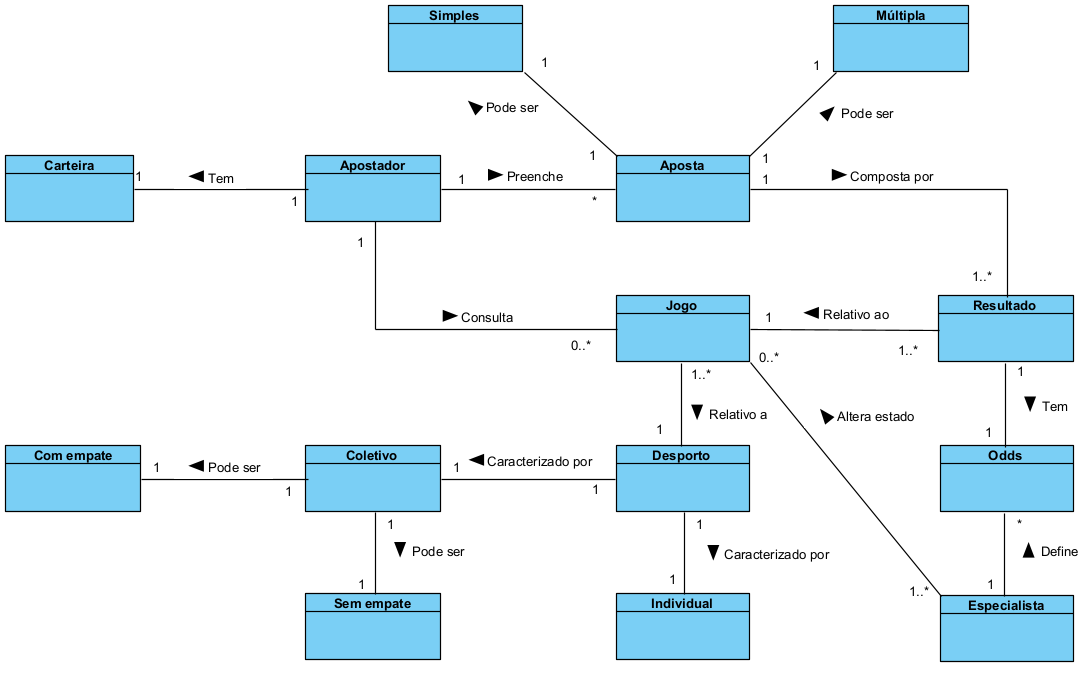
\includegraphics[width=1\linewidth]{imagens/convencao/domainModel.png}
\caption{Modelo de Domínio }
\label{}
\end{figure}%

\section{Definição de entidades}

Nesta secção, são abordadas as diferentes entidades presentes no Modelo de Domínio apresentado na secção anterior (figura 5.1). 

\begin{itemize}
    \item \textbf{Apostador:} Principal utilizador do sistema, cujo proveito da aplicação é tirado por este, na medida em que é o usufruidor da aplicação;
    \item \textbf{Especialista:} Utilizador encarregue das \textit{odds};
    \item \textbf{Administrador:}  Utilizador responsável pela alteração do estado da aposta, ou seja, se esta está ativa, fechada, ou suspensa. Este também é responsável pela gestão de notificações e criação de promoções.
    \item \textbf{Carteira:} O Apostador tem uma carteira que guarda o dinheiro que transfere para o \textit{web site} e ganha das apostas;
    \item \textbf{Jogo:} O apostador pode consultar a listagem de jogos, entre os desportos disponíveis. Cada jogo tem resultados disponíveis para seleção/aposta;
    \item \textbf{Aposta:} É a principal atividade e funcionalidade do \textit{site} de apostas. Esta é composta por resultado(s) de jogo(s), podendo ser simples ou múltipla, consoante o número de resultados de jogos diferentes selecionados; 
    \item \textbf{Aposta Simples:} Uma aposta simples contém apenas 1 resultado (Vitória da equipa 1, Empate ou Vitória da equipa 2) de um jogo, o qual deverá ser vencedor para que a sua aposta seja ganha. Os retornos possíveis são calculados multiplicando o valor da sua aposta pela \textit{odd} disponibilizada;
    \item \textbf{Aposta múltipla:} Uma aposta múltipla contém 2 ou mais resultados de jogos diferentes, em que todos terão de ser vencedores para que a aposta seja ganha. O conceito de "multiplicador" é aplicado para o cálculo das \textit{odds} totais do boletim de apostas e, consequentemente, aos seus potenciais ganhos. Estes são calculados multiplicando o valor da sua aposta pelo produto das várias \textit{odds} no boletim de apostas;
    \item \textbf{\textit{Odd}:}  As \textit{Odds} são cotações dadas a determinado jogo, ou seja, de forma simples elas designam as probabilidades de um determinado evento ocorrer;
    \item \textbf{Desporto:} Modalidades disponíveis no RASBet;
    \item \textbf{Desporto Individual:} O desporto individual é  praticado por cada pessoa, separadamente;
    \item \textbf{Desporto Coletivo:} Desporto coletivo são desportos praticados por duas ou mais pessoas;
    \item \textbf{Desporto Coletivo com Empate:} Desporto coletivo com empate são desportos praticados por duas ou mais pessoas, cujo o "Empate" é opção de resultado, ou seja, do formato V1 | X | V2. 
    \item \textbf{Desporto Coletivo sem Empate:} Desporto coletivo sem empate são desportos praticados por duas ou mais pessoas, cujo o "Empate" não é opção de resultado.
    
    \item \textbf{Resultado:} Representa os resultados de jogos, que o apostador pode selecionar/apostar. No caso de ser um jogo de desporto coletivo com empate, este pode selecionar entre os resultados V1, X e V2, no caso de ser um jogo de desporto coletivo sem empate, só pode selecionar entre os resultados V1 e V2. O apostador, numa mesma aposta, só pode selecionar um dos resultados disponíveis em cada jogo consultado, seja numa aposta simples ou múltipla. 
      
    \item \textbf{Notificações:} Notificações do sistema que anunciam o resultado das apostas quando um jogo acaba, e promoções criadas pelo administrador.
\end{itemize}
\chapter{Âmbito do Produto}
\section{Diagrama de \textit{Use Cases}}
De maneira a compreender melhor o contexto do sistema, vai ser apresentado um diagrama de \textit{Use Cases}. Neste vão ser explicitadas algumas das principais funcionalidades do sistema, bem como os atores do mesmo.
Neste diagrama, é ainda possível identificar, quais as funcionalidades a que cada tipo de ator do sistema vai ter acesso.

\begin{figure}[H]
\centering
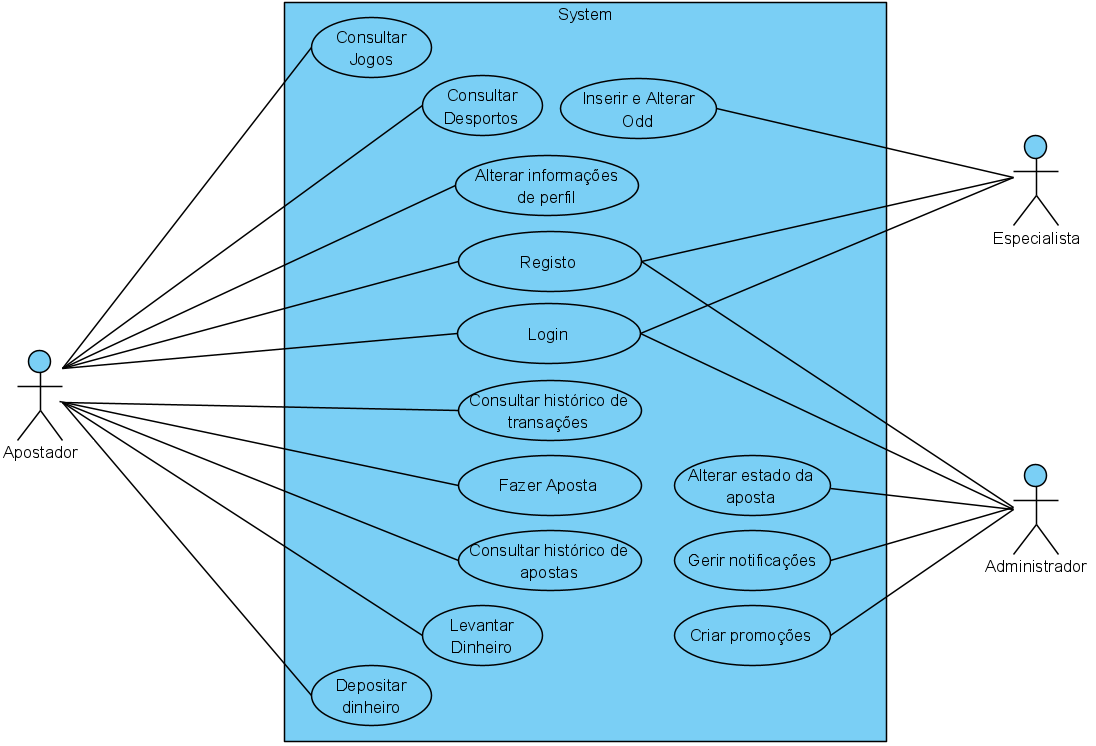
\includegraphics[width=1\textwidth]{imagens/ambitoProduto/Casos_de_uso_NEW.png}
\caption{Diagrama de \textit{Use Cases}}
\end{figure}
\newpage
\section{Atores}
Como está representado no diagrama anterior, o nosso sistema suporta dois tipos de atores: o Apostador e o Especialista. 
\par
O \textbf{Apostador} é o utilizador comum do nosso sistema, vai ter acesso a todas as funcionalidades que a nossa plataforma oferece ao público. 
\par 
O \textbf{Especialista} é o indivíduo que ajustará as \textit{odds} para os futuros jogos, e por isso, para além dessa, as únicas funcionalidades que lhe estão disponíveis são o registo e login.

O \textbf{Administrador} é o indivíduo responsável pela gestão do estado da aposta (suspensa, fechada, ativa), pela gestão das notificações, pela criação de promoções, e por isso, para além dessas, as únicas funcionalidades que lhe estão disponíveis são o registo e login.

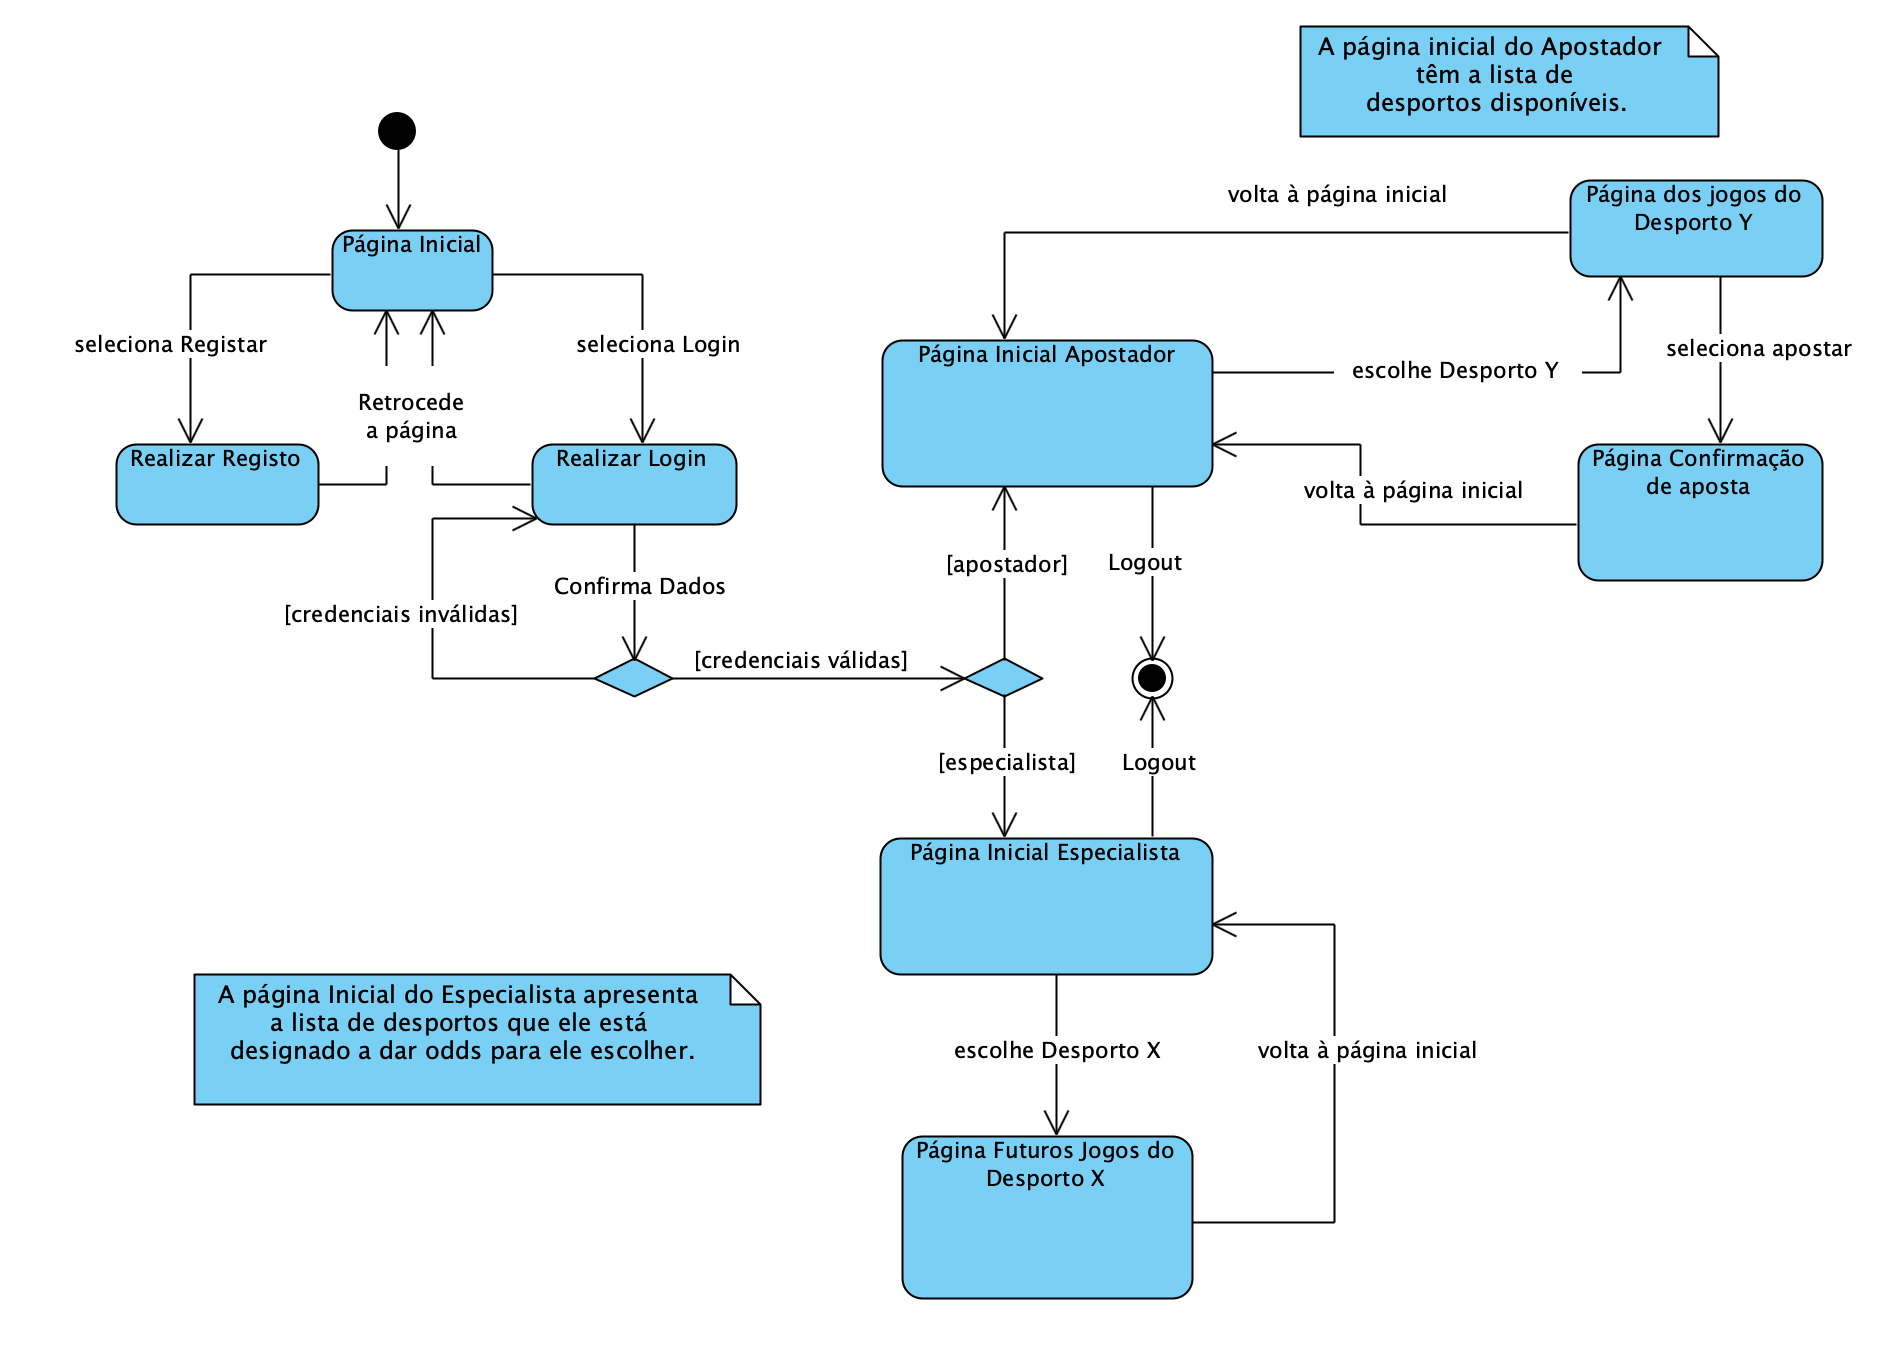
\includegraphics[width=1\textwidth]{imagens/ambitoProduto/maqEstados.png}


\section{Breve Descrição dos Use Cases}
Nesta secção será apresentada uma especificação tabelar de cada \textit{Use Case} considerado, de modo a facilitar todo o processo de implementação de cada funcionalidade do nosso sistema.\\
Deste modo, consideramos que é bastante perceptível o fluxo sequencial da interacção do ator com o sistema.

\subsection{Registar Apostador}
O \textit{use case} Registar para o ator Apostador consiste no registo de um apostador, que ainda não se encontra no sistema.\\
Os casos de erro acontecem quando o sistema deteta uma tentativa de inserir um apostador que já se encontra registado ou caso a \textit{password} pretendida não cumpra os requisitos impostos pelo grupo de uma \textit{password} válida.

\begin{table}[H]
\begin{center}
\scalebox{0.70}{
\begin{tabular}{|l|l|l|}
\hline
\textbf{USE-CASE:} & \multicolumn{2}{l|}{Registar} \\ \hline
\textbf{Ator:} & \multicolumn{2}{l|}{apostador} \\ \hline
\textbf{Pré-Condição:} & \multicolumn{2}{l|}{Ator não está registado no sistema} \\ \hline
\textbf{Pós-Condição:} & \multicolumn{2}{l|}{Ator está registado} \\ \hline
%\multirow 
{\textbf{Cenário Normal}} & \textbf{Ator Input} & \textbf{System Response} \\ \cline{2-3}
& 2 - Fornece credenciais. & \begin{tabular}[c]{@{}l@{}}1- Pede credenciais de  acesso.\\ \\ \\ \\ 3 - Valida credenciais.\\ 4 - Informa que o apostador está registado.\end{tabular} \\ \hline
\begin{tabular}[c]{@{}l@{}}\textbf{Exceção 1 :} {[}username existente{]}\\ (Passo 3)\end{tabular} &  & \begin{tabular}[c]{@{}l@{}}3.1 - Informa o apostador que o username já \\ existe no sistema.\end{tabular} \\ \hline
\begin{tabular}[c]{@{}l@{}}\textbf{Exceção 2 :} {[}password inválida{]}\\  (passo 3)\end{tabular} &  & \begin{tabular}[c]{@{}l@{}}3.2 - Informa o apostador que a password não cumpre\\ os requisitos necessários.\end{tabular} \\ \hline
\end{tabular}}
\caption{Especificação de \textit{Use Case} Registar Apostador}
\end{center}
\end{table}

\newpage
\subsection{Login Apostador}
O \textit{use case} Login Apostador consiste na autenticação de um apostador que se encontra no sistema, sendo o seu login feito através dos seguintes parâmetros : email e \textit{password}.
Os casos de erro acontecem quando o sistema deteta uma tentativa de autenticar um apostador que não se encontra registado ou caso a \textit{password} do apostador não seja correspondente com a que existe no sistema.
\begin{table}[H]
\begin{center}
\scalebox{0.80}{
\begin{tabular}{|p{50mm}|p{40mm}|p{80mm}|}
\hline
\textbf{USE-CASE:} & \multicolumn{2}{l|}{Login} \\ \hline
\textbf{Ator:} & \multicolumn{2}{l|}{Apostador} \\ \hline
\textbf{Pré-Condição:} & \multicolumn{2}{l|}{Ator não está autenticado} \\ \hline
\textbf{Pós-Condição:} & \multicolumn{2}{l|}{Ator está autenticado} \\ \hline
%\multirow
{\textbf{Cenário Normal}} & \textbf{Ator Input} & \textbf{System Response} \\ \cline{2-3}
& 2 - Fornece credenciais. & \begin{tabular}[c]{@{}l@{}}1- Pede credenciais de acesso.\\ \\ 3 - Valida credenciais.\\ 4 - Informa que o apostador está autenticado.\end{tabular} \\ \hline
\begin{tabular}[c]{@{}l@{}}\textbf{Alternativa 1 :}  \\{[}password incorreta{]}\\  (passo 3)\end{tabular} &  & \begin{tabular}[c]{@{}l@{}}3.1 - Informa o apostador que a password \\ não corresponde ao email fornecido. \\3.2- Voltar ao passo 2 \end{tabular} \\ \hline
\begin{tabular}[c]{@{}l@{}}\textbf{Exceção 1 :}\\ {[}email inexistente]\\ (Passo 3){]}\end{tabular} &  & \begin{tabular}[c]{@{}l@{}}3.1.1 - Informa o apostador que o email \\ não existe no sistema.\end{tabular} \\ \hline
\end{tabular}}
\end{center}
\caption{Especificação de \textit{Use Case} Login Apostador}
\end{table}

\subsection{Login Especialista}
O \textit{use case} Login Especialista consiste na autenticação de um especialista com credenciais de acesso para entrar no sistema, sendo o seu login feito através dos seguintes parâmetros : email e \textit{password}.
Os casos de erro acontecem quando o sistema deteta uma tentativa de autenticar um especialista cujo o email não consta no sistema ou caso a \textit{password} do especialista não seja correspondente com a que existe no sistema.
\begin{table}[H]
\begin{center}
\scalebox{0.80}{
\begin{tabular}{|p{50mm}|p{40mm}|p{80mm}|}
\hline
\textbf{USE-CASE:} & \multicolumn{2}{l|}{Login} \\ \hline
\textbf{Ator:} & \multicolumn{2}{l|}{Especialista} \\ \hline
\textbf{Pré-Condição:} & \multicolumn{2}{l|}{Ator não está autenticado} \\ \hline
\textbf{Pós-Condição:} & \multicolumn{2}{l|}{Ator está autenticado} \\ \hline
%\multirow
{\textbf{Cenário Normal}} & \textbf{Ator Input} & \textbf{System Response} \\ \cline{2-3}
& 2 - Fornece credenciais. & \begin{tabular}[c]{@{}l@{}}1- Pede credenciais de acesso.\\ \\ 3 - Valida credenciais.\\ 4 - Informa que o especialista está autenticado.\end{tabular} \\ \hline
\begin{tabular}[c]{@{}l@{}}\textbf{Alternativa 1 :}  \\{[}password incorreta{]}\\  (passo 3)\end{tabular} &  & \begin{tabular}[c]{@{}l@{}}3.1 - Informa o especialista que a password \\ não corresponde ao email fornecido. \\3.2- Voltar ao passo 2 \end{tabular} \\ \hline
\begin{tabular}[c]{@{}l@{}}\textbf{Exceção 1 :}\\ {[}email inexistente]\\ (Passo 3)\end{tabular} &  & \begin{tabular}[c]{@{}l@{}}3.1.1 - Informa o especialista que o email \\ não existe no sistema.\end{tabular} \\ \hline
\end{tabular}}
\end{center}
\caption{Especificação de \textit{Use Case} Login Especialista}
\end{table}

\newpage
\subsection{Login Administrador}
O \textit{use case} Login Administrador consiste na autenticação de um administrador com credenciais de acesso para entrar no sistema, sendo o seu login feito através dos seguintes parâmetros : email e \textit{password}.
Os casos de erro acontecem quando o sistema deteta uma tentativa de autenticar um administrador cujo o email não consta no sistema ou caso a \textit{password} do especialista não seja correspondente com a que existe no sistema.
\begin{table}[H]
\begin{center}
\scalebox{0.80}{
\begin{tabular}{|p{50mm}|p{40mm}|p{80mm}|}
\hline
\textbf{USE-CASE:} & \multicolumn{2}{l|}{Login} \\ \hline
\textbf{Ator:} & \multicolumn{2}{l|}{Especialista} \\ \hline
\textbf{Pré-Condição:} & \multicolumn{2}{l|}{Ator não está autenticado} \\ \hline
\textbf{Pós-Condição:} & \multicolumn{2}{l|}{Ator está autenticado} \\ \hline
%\multirow
{\textbf{Cenário Normal}} & \textbf{Ator Input} & \textbf{System Response} \\ \cline{2-3}
& 2 - Fornece credenciais. & \begin{tabular}[c]{@{}l@{}}1- Pede credenciais de acesso.\\ \\ 3 - Valida credenciais.\\ 4 - Informa que o administrador está autenticado.\end{tabular} \\ \hline
\begin{tabular}[c]{@{}l@{}}\textbf{Alternativa 1 :}  \\{[}password incorreta{]}\\  (passo 3)\end{tabular} &  & \begin{tabular}[c]{@{}l@{}}3.1 - Informa o administrador que a password \\ não corresponde ao email fornecido. \\3.2- Voltar ao passo 2 \end{tabular} \\ \hline
\begin{tabular}[c]{@{}l@{}}\textbf{Exceção 1 :}\\ {[}email inexistente]\\ (Passo 3)\end{tabular} &  & \begin{tabular}[c]{@{}l@{}}3.1.1 - Informa o administrador que o email \\ não existe no sistema.\end{tabular} \\ \hline
\end{tabular}}
\end{center}
\caption{Especificação de \textit{Use Case} Login Administrador}
\end{table}

\newpage
\subsection{Alterar informações de perfil}
O \textit{use case} Alterar informações de perfil consiste no apostador alterar os parâmetros editáveis do seu perfil, que são o nome e o email (cenário normal). Caso este pretenda alterar a morada ou o número de telemóvel, só o poderá fazer com passos adicionais "mais seguros", para confirmar a sua identidade, como por exemplo, receber uma mensagem com um código para proceder à sua alteração (cenário adicional). Dados mais "sensíveis" como Nº de Identificação Fiscal, Nº do Cartão de cidadão e Data de Nascimento não são editáveis.
\begin{table}[H]
\begin{center}
\scalebox{0.80}{
\begin{tabular}{|p{40mm}|p{50mm}|p{80mm}|}
\hline
\textbf{USE-CASE:} & \multicolumn{2}{l|}{Alterar informações de perfil} \\ \hline
\textbf{Ator:} & \multicolumn{2}{l|}{Apostador} \\ \hline
\textbf{Pré-Condição:} & \multicolumn{2}{l|}{Ator autenticado} \\ \hline
\textbf{Pós-Condição:} & \multicolumn{2}{l|}{Ator contém informações de perfil editadas} \\ \hline
%\multirow
{\textbf{Cenário Normal}} & \textbf{Ator Input} & \textbf{System Response} \\ \cline{2-3}
& \begin{tabular}[c]{@{}l@{}} 1 - Informa o sistema que \\ pretende editar as suas\\ informações. \\ \\  3- Altera informações. \\ 4 - Guarda alterações.  \end{tabular}&  \begin{tabular}[c]{@{}l@{}} \\ \\ \\2 - Apresenta campos de informação em modo \\de edição.\\ \\ \\ \\5 - Informa que as alterações foram guardadas.\end{tabular} \\ \hline
%\multirow
{\textbf{Cenário Adicional}} & \textbf{Ator Input} & \textbf{System Response} \\ \cline{2-3}
& \begin{tabular}[c]{@{}l@{}} 1 - Informa o sistema que \\ pretende editar as suas\\ informações. \\ 3 - Preenche o campo com o \\que é pedido. \\ 5 - Coloca o código no campo. \\ 7 - Altera as informações. \\ 8 - Guarda as alterações. \end{tabular}&  \begin{tabular}[c]{@{}l@{}} 2 - Apresenta um campo para que o utilizador\\insira o número de telemóvel.\\ 4 - O sistema envia um código para o \\ respetivo número. \\6 - Apresenta campos de informação em \\ modo de edição. \\ 9 - Informa que as alterações foram guardadas. \end{tabular} \\ \hline
\end{tabular}}
\end{center}
\caption{Especificação de \textit{Use Case} Alterar informações de perfil}
\end{table}

\subsection{Consultar jogos}
O \textit{use case} Consultar jogos permite ao utilizador selecionar um ou mais desportos e ver a lista de jogos desse(s) desporto(s).
\begin{table}[H]
\begin{center}
\scalebox{0.80}{
\begin{tabular}{|p{40mm}|p{70mm}|p{80mm}|}
\hline
\textbf{USE-CASE:} & \multicolumn{2}{l|}{Consultar jogos} \\ \hline
\textbf{Ator:} & \multicolumn{2}{l|}{Apostador} \\ \hline
\textbf{Pré-Condição:} & \multicolumn{2}{l|}{Ator autenticado} \\ \hline
\textbf{Pós-Condição:} & \multicolumn{2}{l|}{Ator acede a uma lista de jogos} \\ \hline
%\multirow
{\textbf{Cenário Normal}} & \textbf{Ator Input} & \textbf{System Response} \\ \cline{2-3}
& \begin{tabular}[c]{@{}l@{}} 1 - Informa o sistema qual o desporto\\ que pretende consultar.   \end{tabular}&  \begin{tabular}[c]{@{}l@{}}\\ \\ \\ \\2 - Apresenta a lista de jogos desse desporto.\end{tabular} \\ \hline
\end{tabular}}
\end{center}
\caption{Especificação de\textit{ Use Case} Consultar jogos}
\end{table}

\newpage
\subsection{Fazer aposta}
O \textit{use case} Fazer aposta consiste no utilizador selecionar um resultado de jogo, escolher a quantia a apostar e efetuar o pagamento da mesma.
\begin{table}[H]
\begin{center}
\scalebox{0.80}{
\begin{tabular}{|p{40mm}|p{50mm}|p{80mm}|}
\hline
\textbf{USE-CASE:} & \multicolumn{2}{l|}{Consultar jogos} \\ \hline
\textbf{Ator:} & \multicolumn{2}{l|}{Apostador} \\ \hline
\textbf{Pré-Condição:} & \multicolumn{2}{l|}{Ator autenticado} \\ \hline
\textbf{Pós-Condição:} & \multicolumn{2}{l|}{Ator obtém confirmação de aposta} \\ \hline
%\multirow
{\textbf{Cenário Normal}} & \textbf{Ator Input} & \textbf{System Response} \\ \cline{2-3}
& \begin{tabular}[c]{@{}l@{}} 1 - Informa o sistema qual o \\ jogo e montante que pretende\\ apostar. \\ 2 - Confirma aposta. \\ \\ \\ 4 - Realiza pagamento. \end{tabular}&  \vspace{3.5mm} \begin{tabular}[c]{@{}l@{}} 3 - Solicita pagamento da \\ aposta. \\ \\ 5 - Valida o pagamento. \\ 6- Informa o apostador que a aposta foi \\ realizada com sucesso.\end{tabular} \\ \hline
\begin{tabular}[c]{@{}l@{}}\textbf{Exceção 1 :}\\ {[}método de pagamento \\ inválido]\\ (Passo 5)\end{tabular} &  & \begin{tabular}[c]{@{}l@{}}5.1 - Informa o apostador que o método de \\ pagamento usado não é válido. \\ 5.2 - Volta ao passo 4. \end{tabular} \\ \hline
\end{tabular}}
\end{center}
\caption{Especificação de \textit{Use Case} Fazer aposta}
\end{table}

\subsection{Consultar histórico de apostas}
O \textit{use case} Consultar histórico de apostas consiste em apresentar ao apostador a lista de apostas que ele já realizou no sistema.
\begin{table}[H]
\begin{center}
\scalebox{0.80}{
\begin{tabular}{|p{40mm}|p{60mm}|p{70mm}|}
\hline
\textbf{USE-CASE:} & \multicolumn{2}{l|}{Consultar histórico de apostas} \\ \hline
\textbf{Ator:} & \multicolumn{2}{l|}{Apostador} \\ \hline
\textbf{Pré-Condição:} & \multicolumn{2}{l|}{Ator autenticado} \\ \hline
\textbf{Pós-Condição:} & \multicolumn{2}{l|}{Ator obtém a lista de apostas já realizadas} \\ \hline
%\multirow
{\textbf{Cenário Normal}} & \textbf{Ator Input} & \textbf{System Response} \\ \cline{2-3}
& \begin{tabular}[c]{@{}l@{}} 1 - Informa o sistema a intenção \\ de ver o seu histórico de apostas. \end{tabular} &  \begin{tabular}[c]{@{}l@{}} \\ \\ \\2 - Apresenta a lista de apostas \\ já realizadas pelo apostador.\end{tabular} \\ \hline
\end{tabular}}
\end{center}
\caption{Especificação de \textit{Use Case} Consultar histórico de apostas}
\end{table}

\newpage
\subsection{Consultar histórico de transações}
O \textit{use case} Consultar histórico de transações consiste em apresentar ao apostador os movimentos de dinheiro da sua conta tais como depósitos, levantamentos, ganhos e perdas de apostas.
\begin{table}[H]
\begin{center}
\scalebox{0.80}{
\begin{tabular}{|p{40mm}|p{60mm}|p{70mm}|}
\hline
\textbf{USE-CASE:} & \multicolumn{2}{l|}{Consultar histórico de transações} \\ \hline
\textbf{Ator:} & \multicolumn{2}{l|}{Apostador} \\ \hline
\textbf{Pré-Condição:} & \multicolumn{2}{l|}{Ator autenticado} \\ \hline
\textbf{Pós-Condição:} & \multicolumn{2}{l|}{Ator obtém uma lista de movimentos de conta} \\ \hline
%\multirow
{\textbf{Cenário Normal}} & \textbf{Ator Input} & \textbf{System Response} \\ \cline{2-3}
& \begin{tabular}[c]{@{}l@{}} 1 - Informa o sistema a intenção \\ de ver o seu histórico de transações. \end{tabular} &  \begin{tabular}[c]{@{}l@{}} \\ \\ \\2 - Apresenta a lista de movimentos \\ do apostador.\end{tabular} \\ \hline
\end{tabular}}
\end{center}
\caption{Especificação de \textit{Use Case} Consultar histórico de transações}
\end{table}

\subsection{Depositar dinheiro}
O \textit{use case} Depositar dinheiro consiste na intenção do apostador em adicionar dinheiro ao seu saldo.
\begin{table}[H]
\begin{center}
\scalebox{0.80}{
\begin{tabular}{|p{40mm}|p{55mm}|p{75mm}|}
\hline
\textbf{USE-CASE:} & \multicolumn{2}{l|}{Depositar dinheiro} \\ \hline
\textbf{Ator:} & \multicolumn{2}{l|}{Apostador} \\ \hline
\textbf{Pré-Condição:} & \multicolumn{2}{l|}{Ator autenticado} \\ \hline
\textbf{Pós-Condição:} & \multicolumn{2}{l|}{Ator com mais dinheiro na sua conta} \\ \hline
%\multirow
{\textbf{Cenário Normal}} & \textbf{Ator Input} & \textbf{System Response} \\ \cline{2-3}
& \begin{tabular}[c]{@{}l@{}} 1 - Informa o sistema a intenção \\ de depositar dinheiro. \\ \\ 3 - Realiza transferência. \end{tabular} &  \begin{tabular}[c]{@{}l@{}} \\ \\ \\ \\ \\ 2 - Solicita a escolha do montante \\ e forma de transferência. \\ \\ 4 - Valida transferência. \\ 5 -  Informa o apostador que a transferência \\  foi realizada com sucesso.\end{tabular} \\ \hline
\begin{tabular}[c]{@{}l@{}}\textbf{Exceção 1 :}\\ {[}método de pagamento \\ inválido]\\ (Passo 4)\end{tabular} &  & \begin{tabular}[c]{@{}l@{}}4.1 - Informa o apostador que o método de \\ transferência usado não é válido. \\ 4.2 - Volta ao passo 3. \end{tabular} \\ \hline
\end{tabular}}
\end{center}
\caption{Especificação de \textit{Use Case} Depositar dinheiro}
\end{table}

\newpage
\subsection{Levantar dinheiro}
O \textit{use case} Levantar dinheiro consiste na intenção do apostador em levantar dinheiro da sua conta.
\begin{table}[H]
\begin{center}
\scalebox{0.80}{
\begin{tabular}{|p{40mm}|p{55mm}|p{75mm}|}
\hline
\textbf{USE-CASE:} & \multicolumn{2}{l|}{Levantar dinheiro} \\ \hline
\textbf{Ator:} & \multicolumn{2}{l|}{Apostador} \\ \hline
\textbf{Pré-Condição:} & \multicolumn{2}{l|}{Ator autenticado e com saldo positivo na conta} \\ \hline
\textbf{Pós-Condição:} & \multicolumn{2}{l|}{Ator com menos dinheiro na sua conta} \\ \hline
%\multirow
{\textbf{Cenário Normal}} & \textbf{Ator Input} & \textbf{System Response} \\ \cline{2-3}
& \begin{tabular}[c]{@{}l@{}} 1 - Informa o sistema a intenção \\ de levantar dinheiro. \\ \\ 3 - Realiza transferência. \end{tabular} &  \begin{tabular}[c]{@{}l@{}} \\ \\ \\ \\ \\ 2 - Solicita a escolha do montante \\ e forma de transferência. \\ \\ 4 - Valida transferência. \\ 5 -  Informa o apostador que a transferência \\  foi realizada com sucesso.\end{tabular} \\ \hline
\begin{tabular}[c]{@{}l@{}}\textbf{Exceção 1 :}\\ {[}método de pagamento \\ inválido]\\ (Passo 4)\end{tabular} &  & \begin{tabular}[c]{@{}l@{}}4.1 - Informa o apostador que o método de \\ transferência usado não é válido. \\ 4.2 - Volta ao passo 3. \end{tabular} \\ \hline
\end{tabular}}
\end{center}
\caption{Especificação de \textit{Use Case} Levantar dinheiro}
\end{table}

\subsection{Inserir \textit{odd}}
O \textit{use case} Inserir \textit{odd} apenas está disponível para o Especialista e consiste neste fixar a \textit{odd} de jogos futuros.
\begin{table}[H]
\begin{center}
\scalebox{0.80}{
\begin{tabular}{|p{40mm}|p{60mm}|p{70mm}|}
\hline
\textbf{USE-CASE:} & \multicolumn{2}{l|}{Inserir odd} \\ \hline
\textbf{Ator:} & \multicolumn{2}{l|}{Especialista} \\ \hline
\textbf{Pré-Condição:} & \multicolumn{2}{l|}{Ator autenticado} \\ \hline
\textbf{Pós-Condição:} & \multicolumn{2}{l|}{Odds de jogo(s) futuros definida(s)} \\ \hline
%\multirow
{\textbf{Cenário Normal}} & \textbf{Ator Input} & \textbf{System Response} \\ \cline{2-3}
& \begin{tabular}[c]{@{}l@{}} 1 - Escolhe um desporto. \\ \\ \\ 3 - Fixa odd para um ou mais jogos. \\ 4 - Guarda alterações. \end{tabular} &  \begin{tabular}[c]{@{}l@{}} \\ 2 - Apresenta a lista de jogos sem odds \\ do desporto escolhido. \\ \\ \\ 5 - Informa o especialista que as odds \\ foram guardadas com sucesso.\end{tabular} \\ \hline
\end{tabular}}
\end{center}
\caption{Especificação de \textit{Use Case} Inserir \textit{odd}}
\end{table}

\newpage
\subsection{Alterar estado da aposta}
O \textit{use case} Alterar estado da aposta apenas está disponível para o Administrador e consiste neste alterar o estado da aposta (ativa, fechada ou suspensa), no caso de, por exemplo, acontecer alguma situação que leve à sua suspensão.
\begin{table}[H]
\begin{center}
\scalebox{0.80}{
\begin{tabular}{|p{40mm}|p{60mm}|p{70mm}|}
\hline
\textbf{USE-CASE:} & \multicolumn{2}{l|}{Alterar estado da aposta} \\ \hline
\textbf{Ator:} & \multicolumn{2}{l|}{Administrador} \\ \hline
\textbf{Pré-Condição:} & \multicolumn{2}{l|}{Administrador autenticado} \\ \hline
\textbf{Pós-Condição:} & \multicolumn{2}{l|}{Estado da aposta alterado} \\ \hline
%\multirow
{\textbf{Cenário Normal}} & \textbf{Ator Input} & \textbf{System Response} \\ \cline{2-3}
& \begin{tabular}[c]{@{}l@{}} 1 - Informa o sistema a vontade de \\ alterar o estado da aposta. \\ 2 - Ativa, fecha ou suspende a aposta. \\ 3 - Guarda as alterações feitas. \end{tabular} &  \vspace{5mm} \begin{tabular}[c]{@{}l@{}}  4 - Informa o administrador que a operação \\ foi efetuada com sucesso.\end{tabular} \\ \hline
\end{tabular}}
\end{center}
\caption{Especificação de \textit{Use Case} Alterar estado da aposta}
\end{table}

\newpage
\section{Diagramas de Sequência e Mockups}
Os Diagramas de Sequência são Diagramas de Interação cujo foco é, principalmente, a ordenação temporal das mensagens e representação das mesmas.
Desta forma, tendo por base o nosso Diagrama de Classes, desenvolvemos os seguintes Diagramas de Sequência representativos do funcionamento do sistema.

\subsection{Registo Apostador}
\begin{figure}[H]
\centering
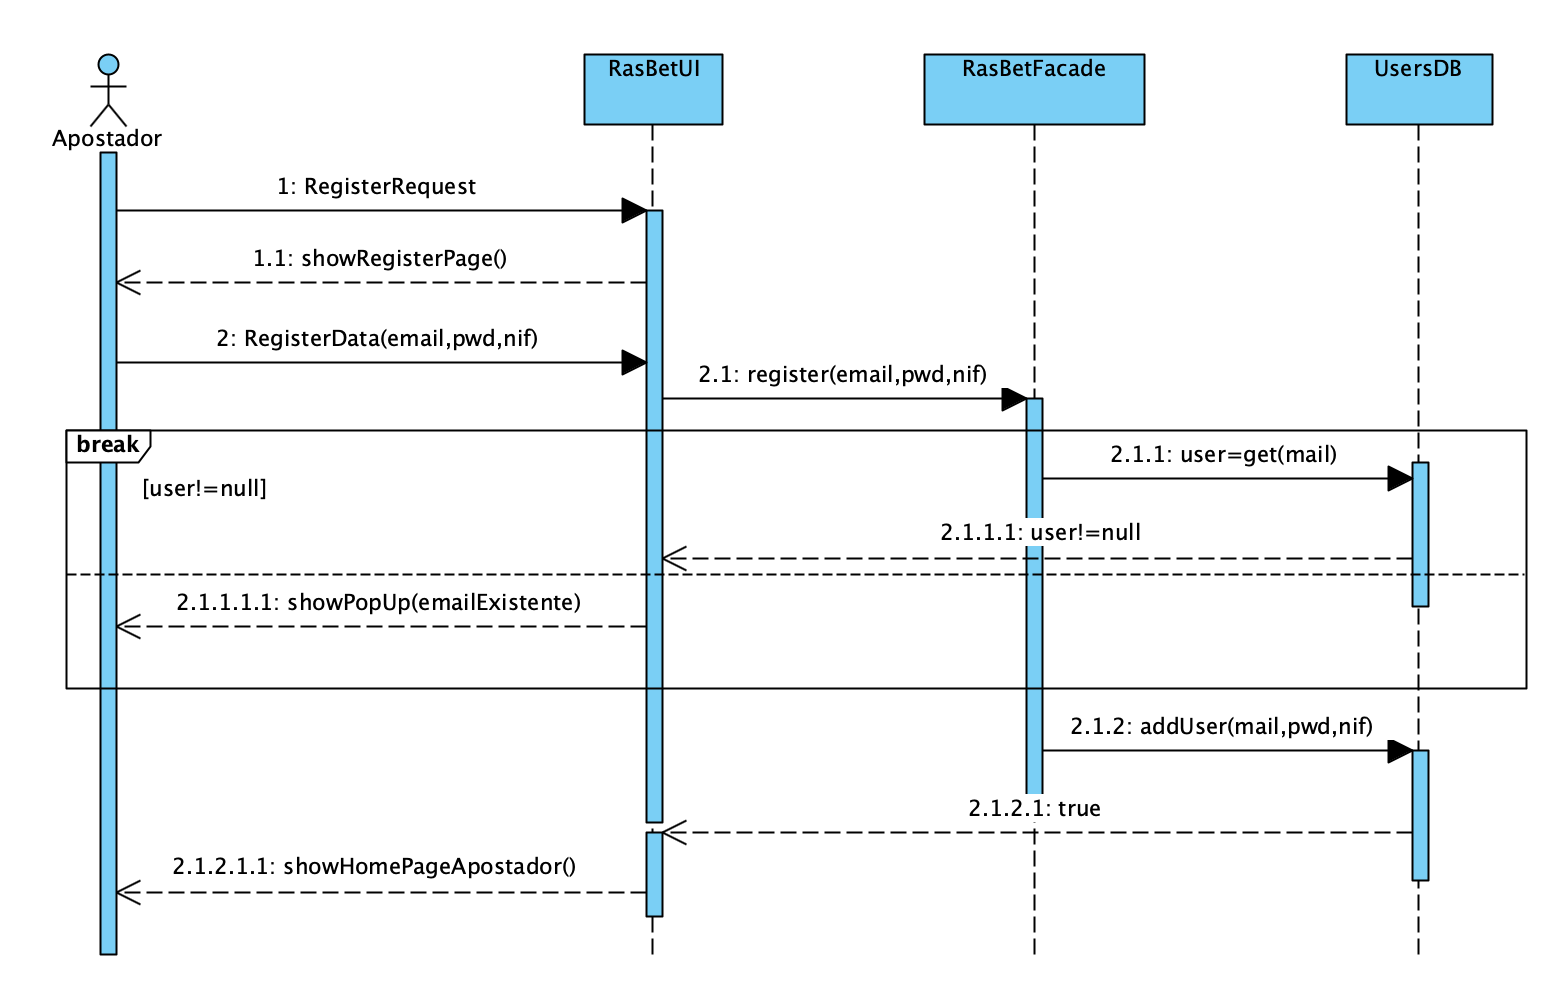
\includegraphics[width=0.8\textwidth]{imagens/ambitoProduto/SRegisto.png}
\caption{Diagrama de Sequência de Registo}
\end{figure}
\begin{figure}[H]
\centering
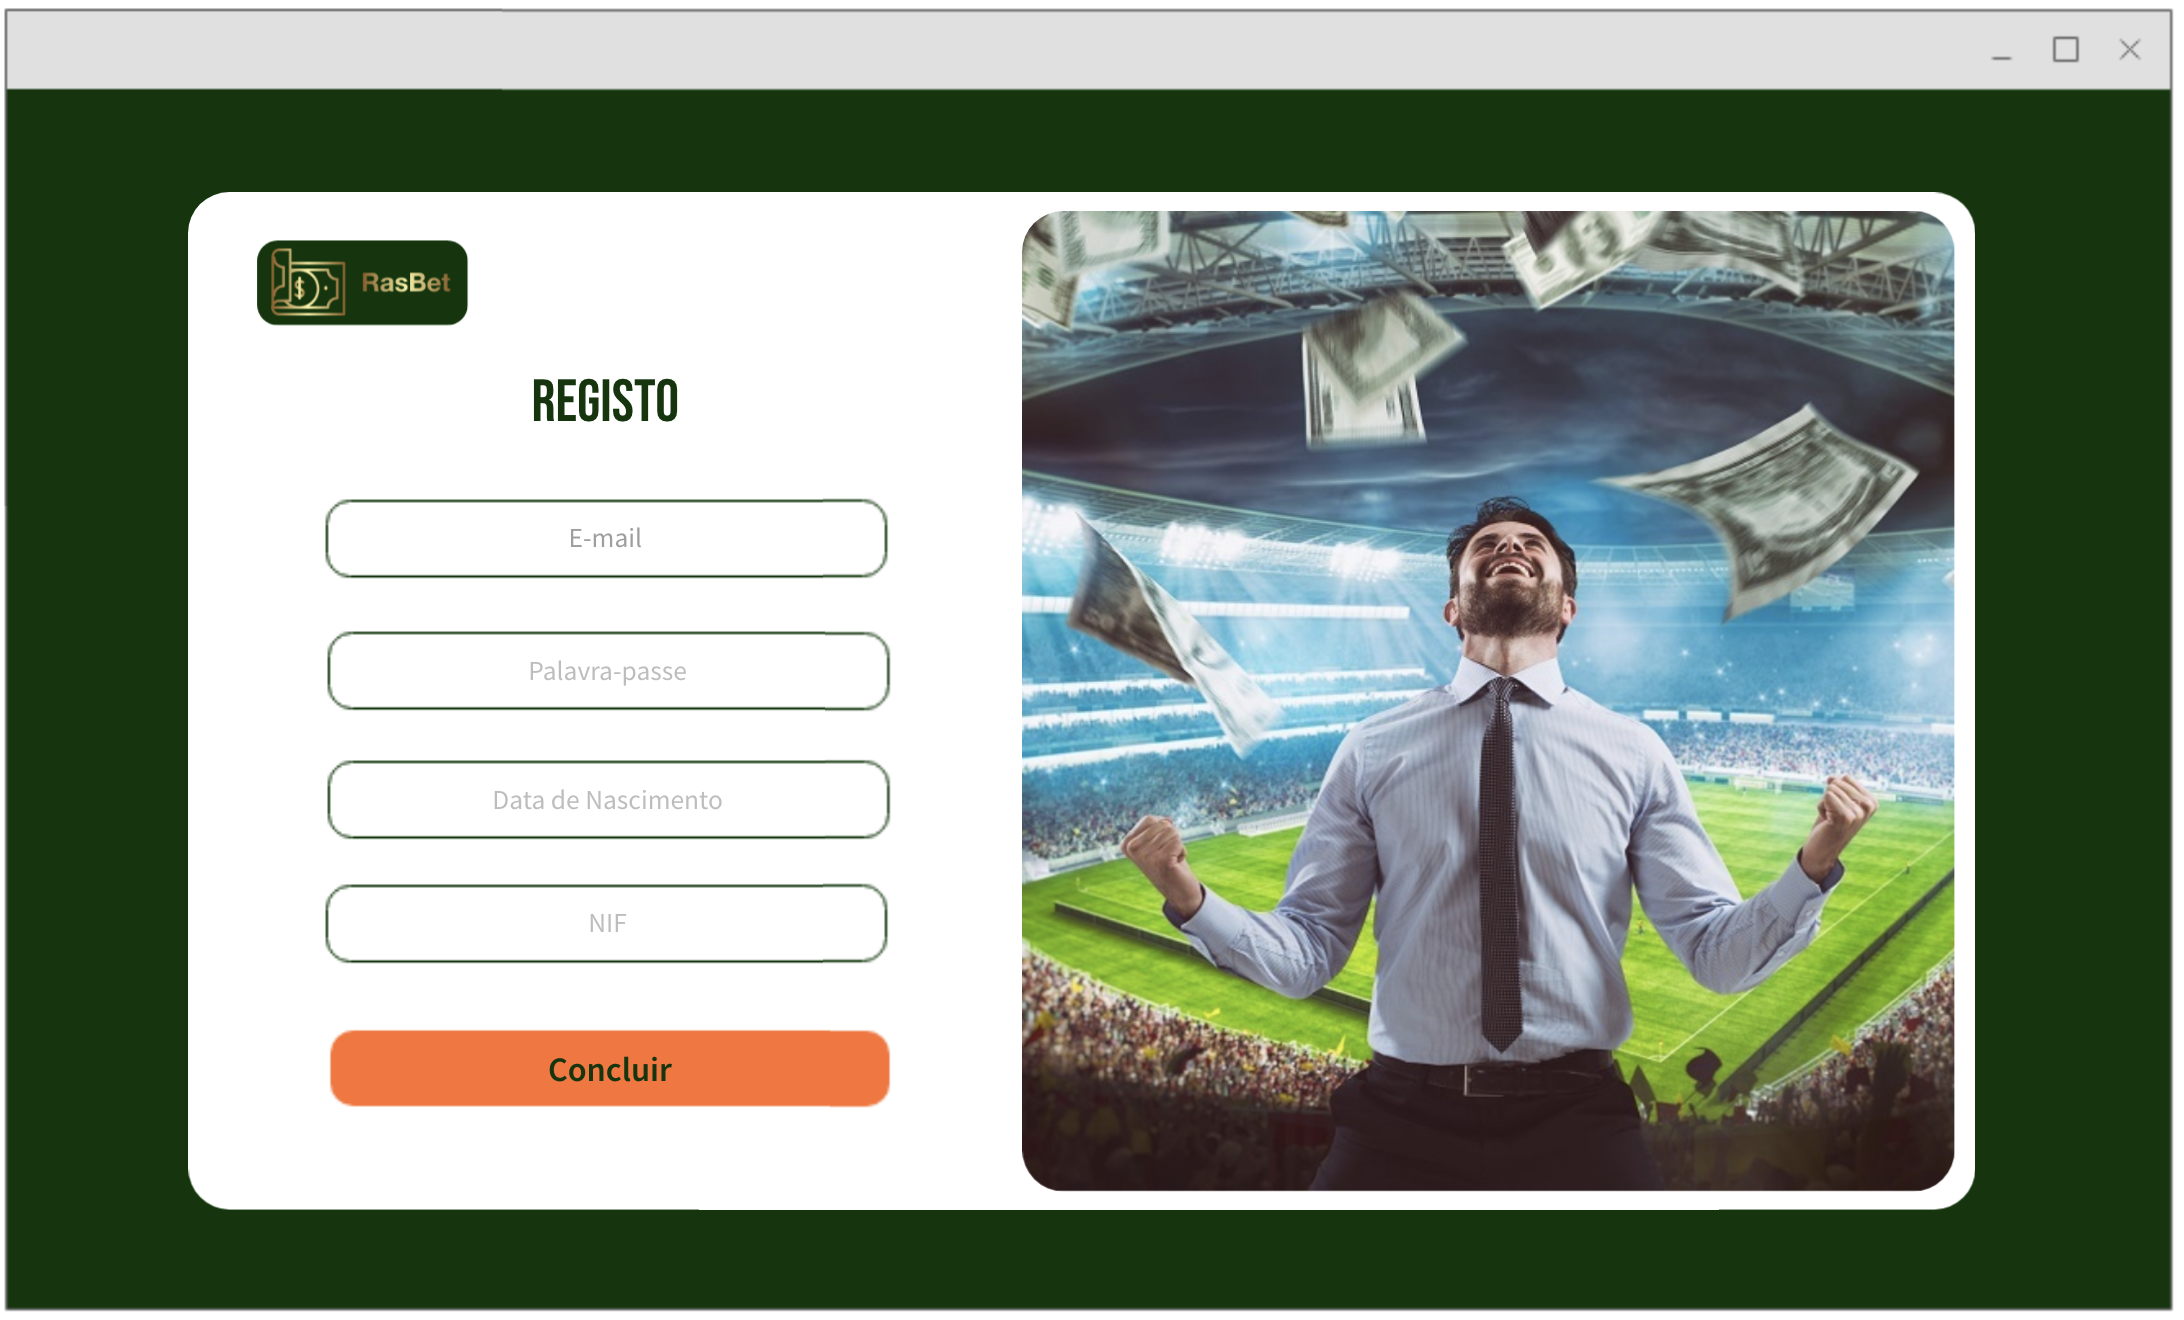
\includegraphics[width=0.9\textwidth]{imagens/ambitoProduto/Mockups/M_Registo.png}
\caption{Mockup de Registo}
\end{figure}

\subsection{Login Apostador/Especialista}
\begin{figure}[H]
\centering
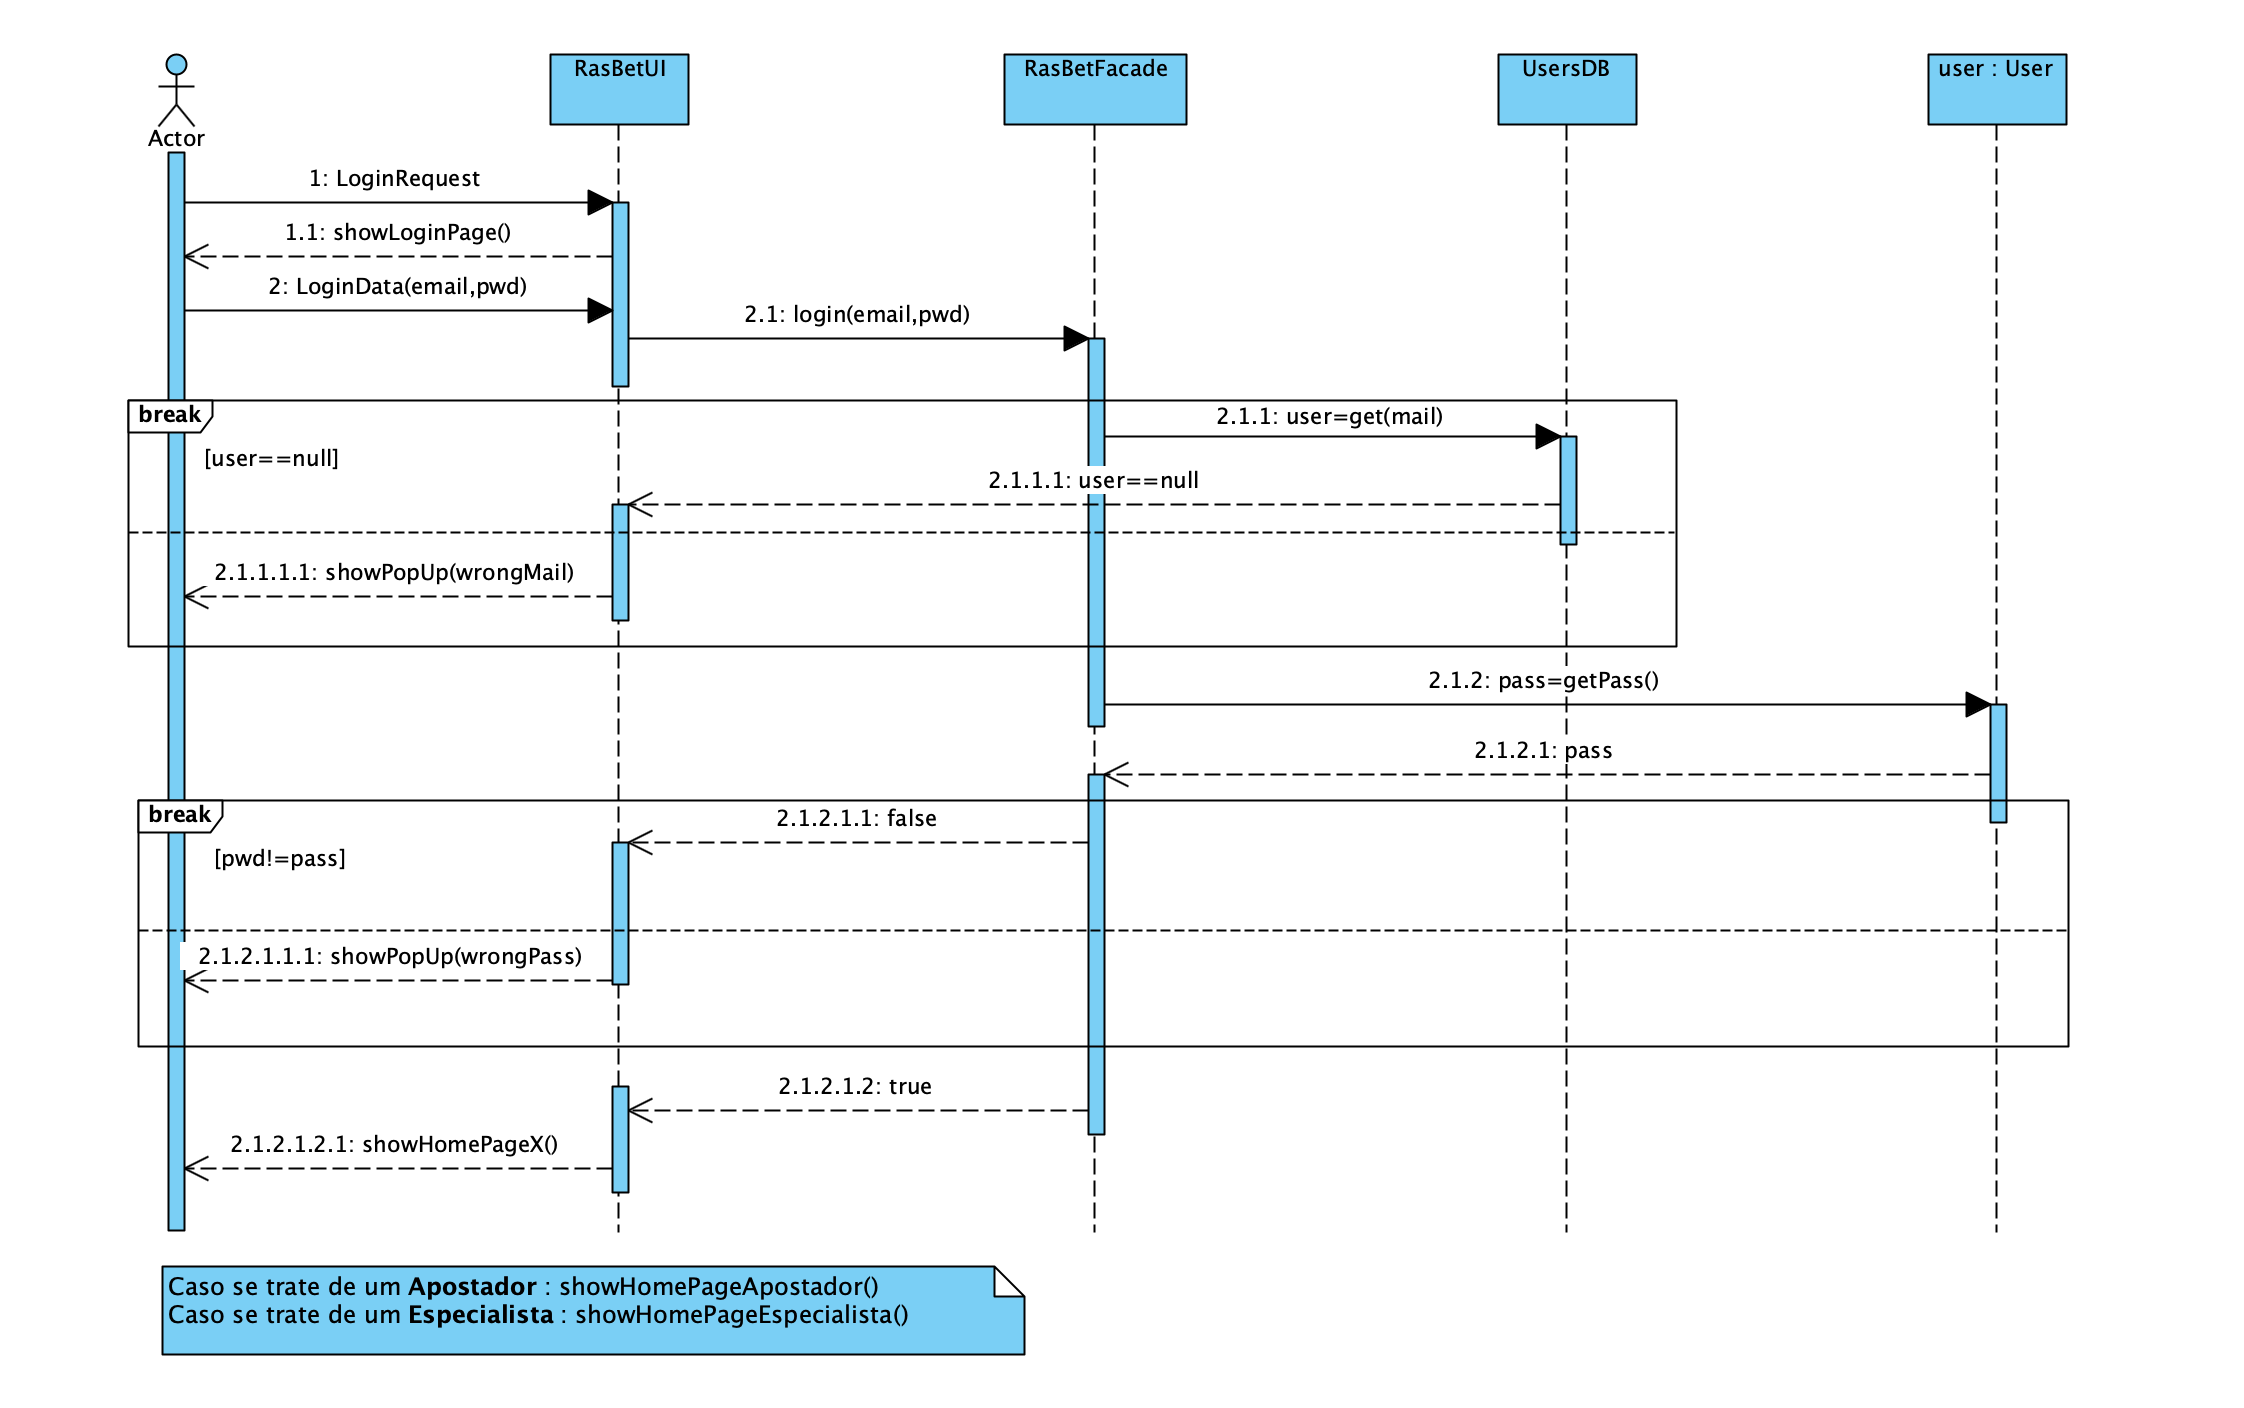
\includegraphics[width=1\textwidth]{imagens/ambitoProduto/SLogin.png}
\caption{Diagrama de Sequência de Login}
\end{figure}
\begin{figure}[H]
\centering
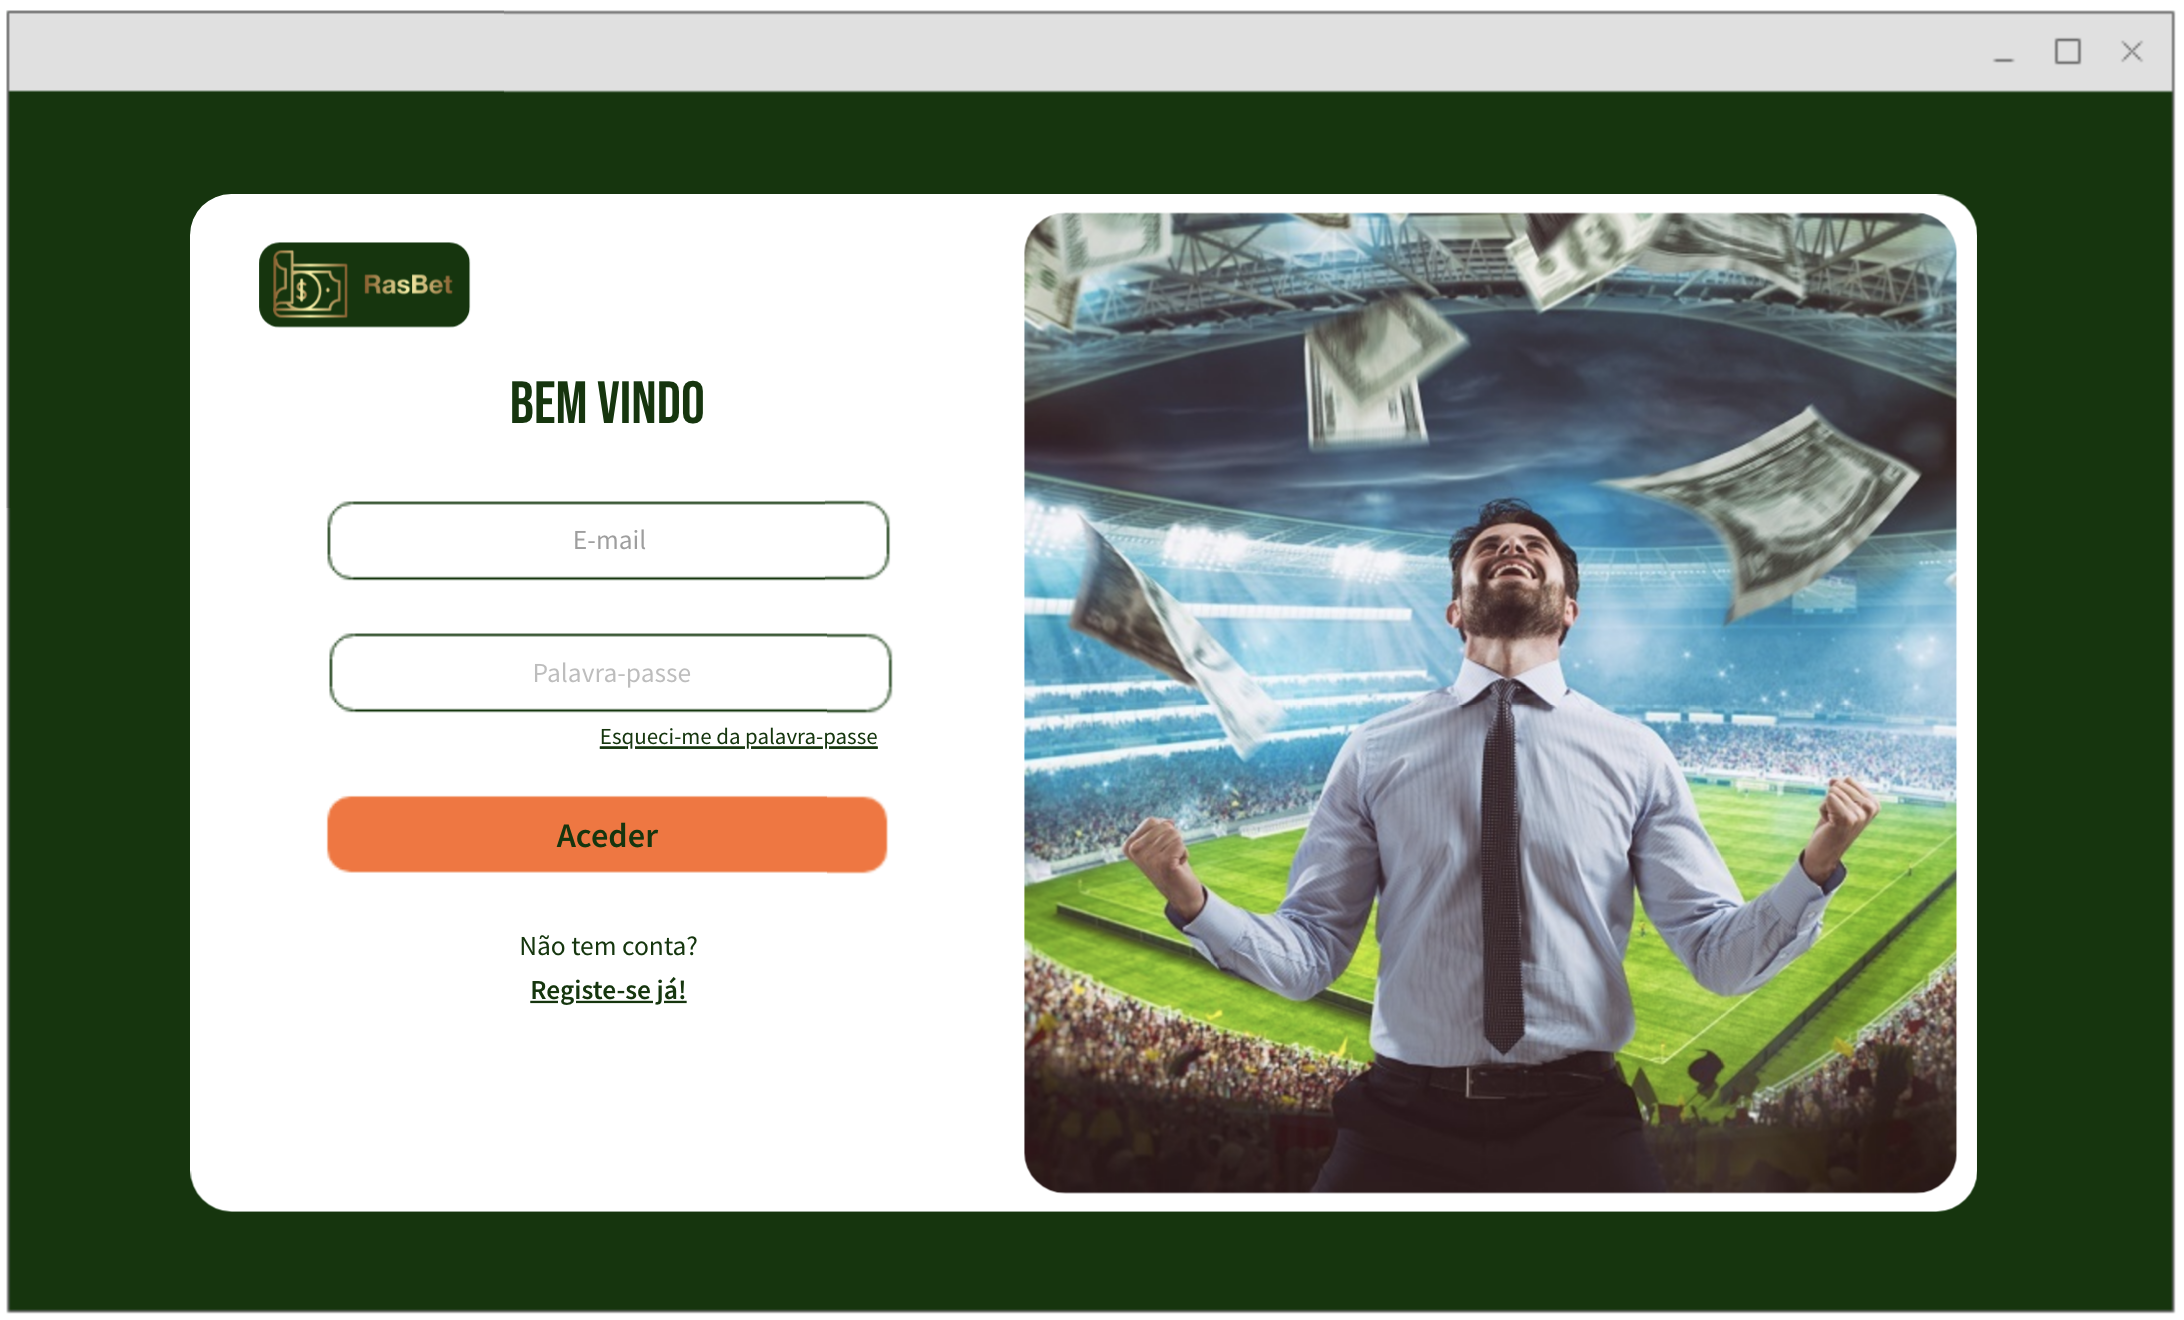
\includegraphics[width=1\textwidth]{imagens/ambitoProduto/Mockups/M_Login.png}
\caption{Mockup de Login}
\end{figure}

\subsection{Alterar informações de perfil}
\begin{figure}[H]
\centering
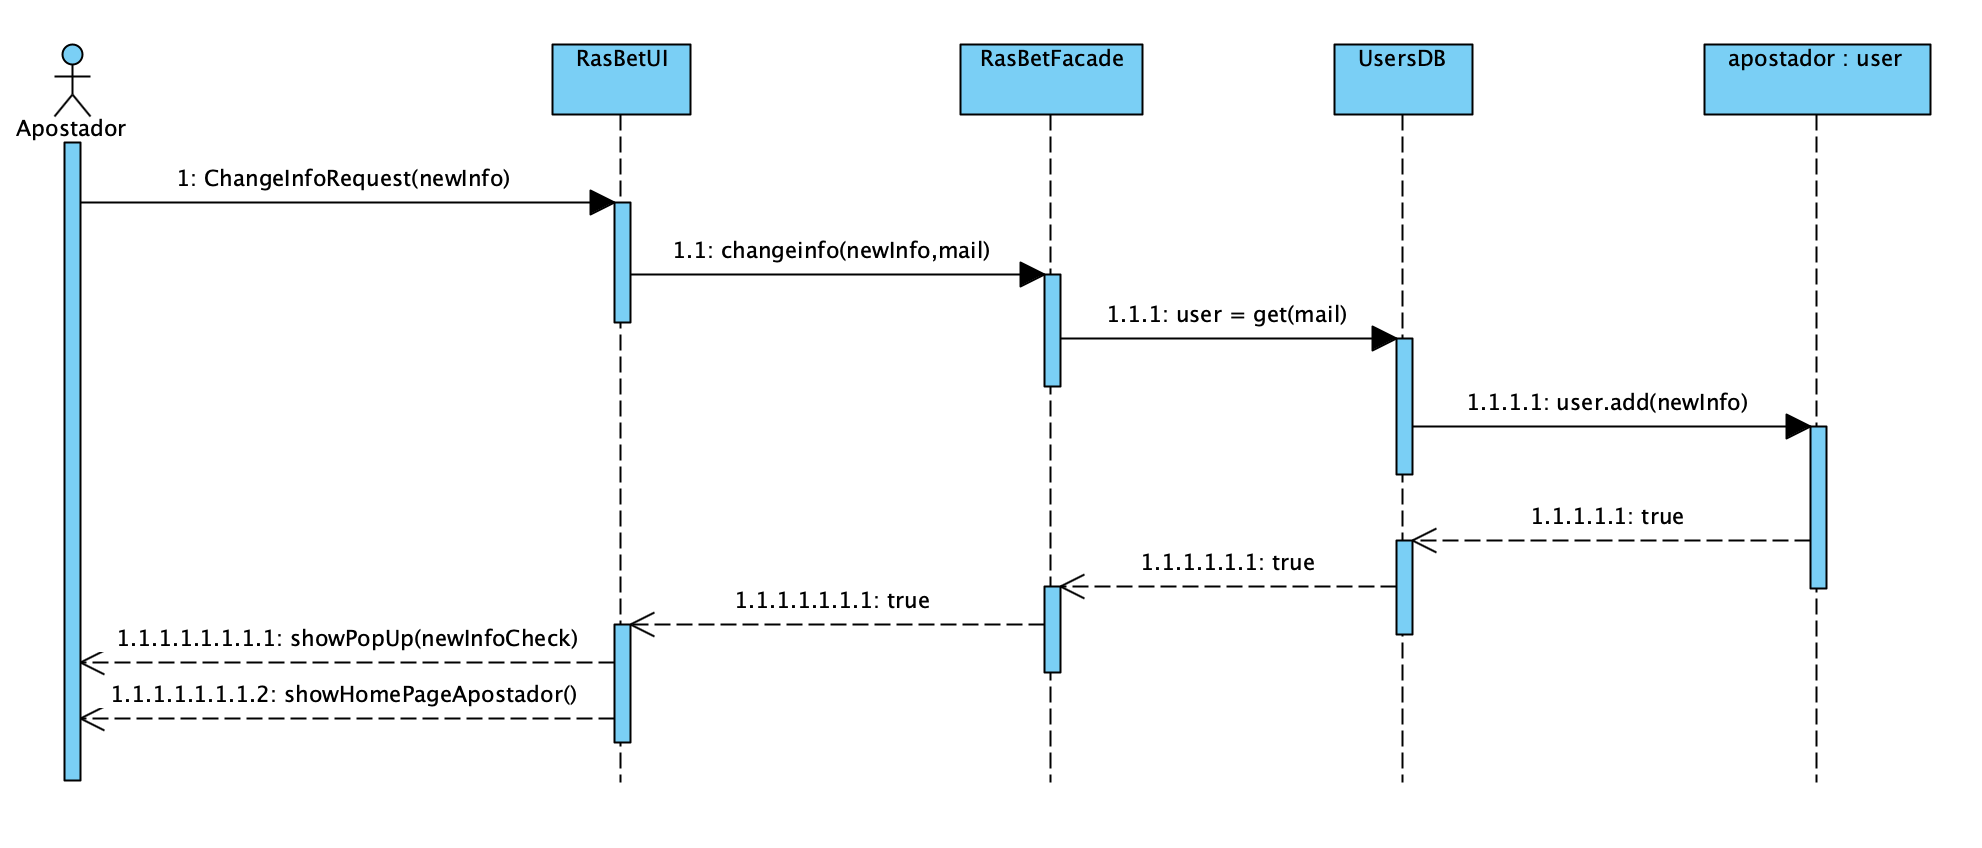
\includegraphics[width=1\textwidth]{imagens/ambitoProduto/SalterarInfo.png}
\caption{Diagrama de Sequência de alterar informações de perfil}
\end{figure}
\begin{figure}[H]
\centering
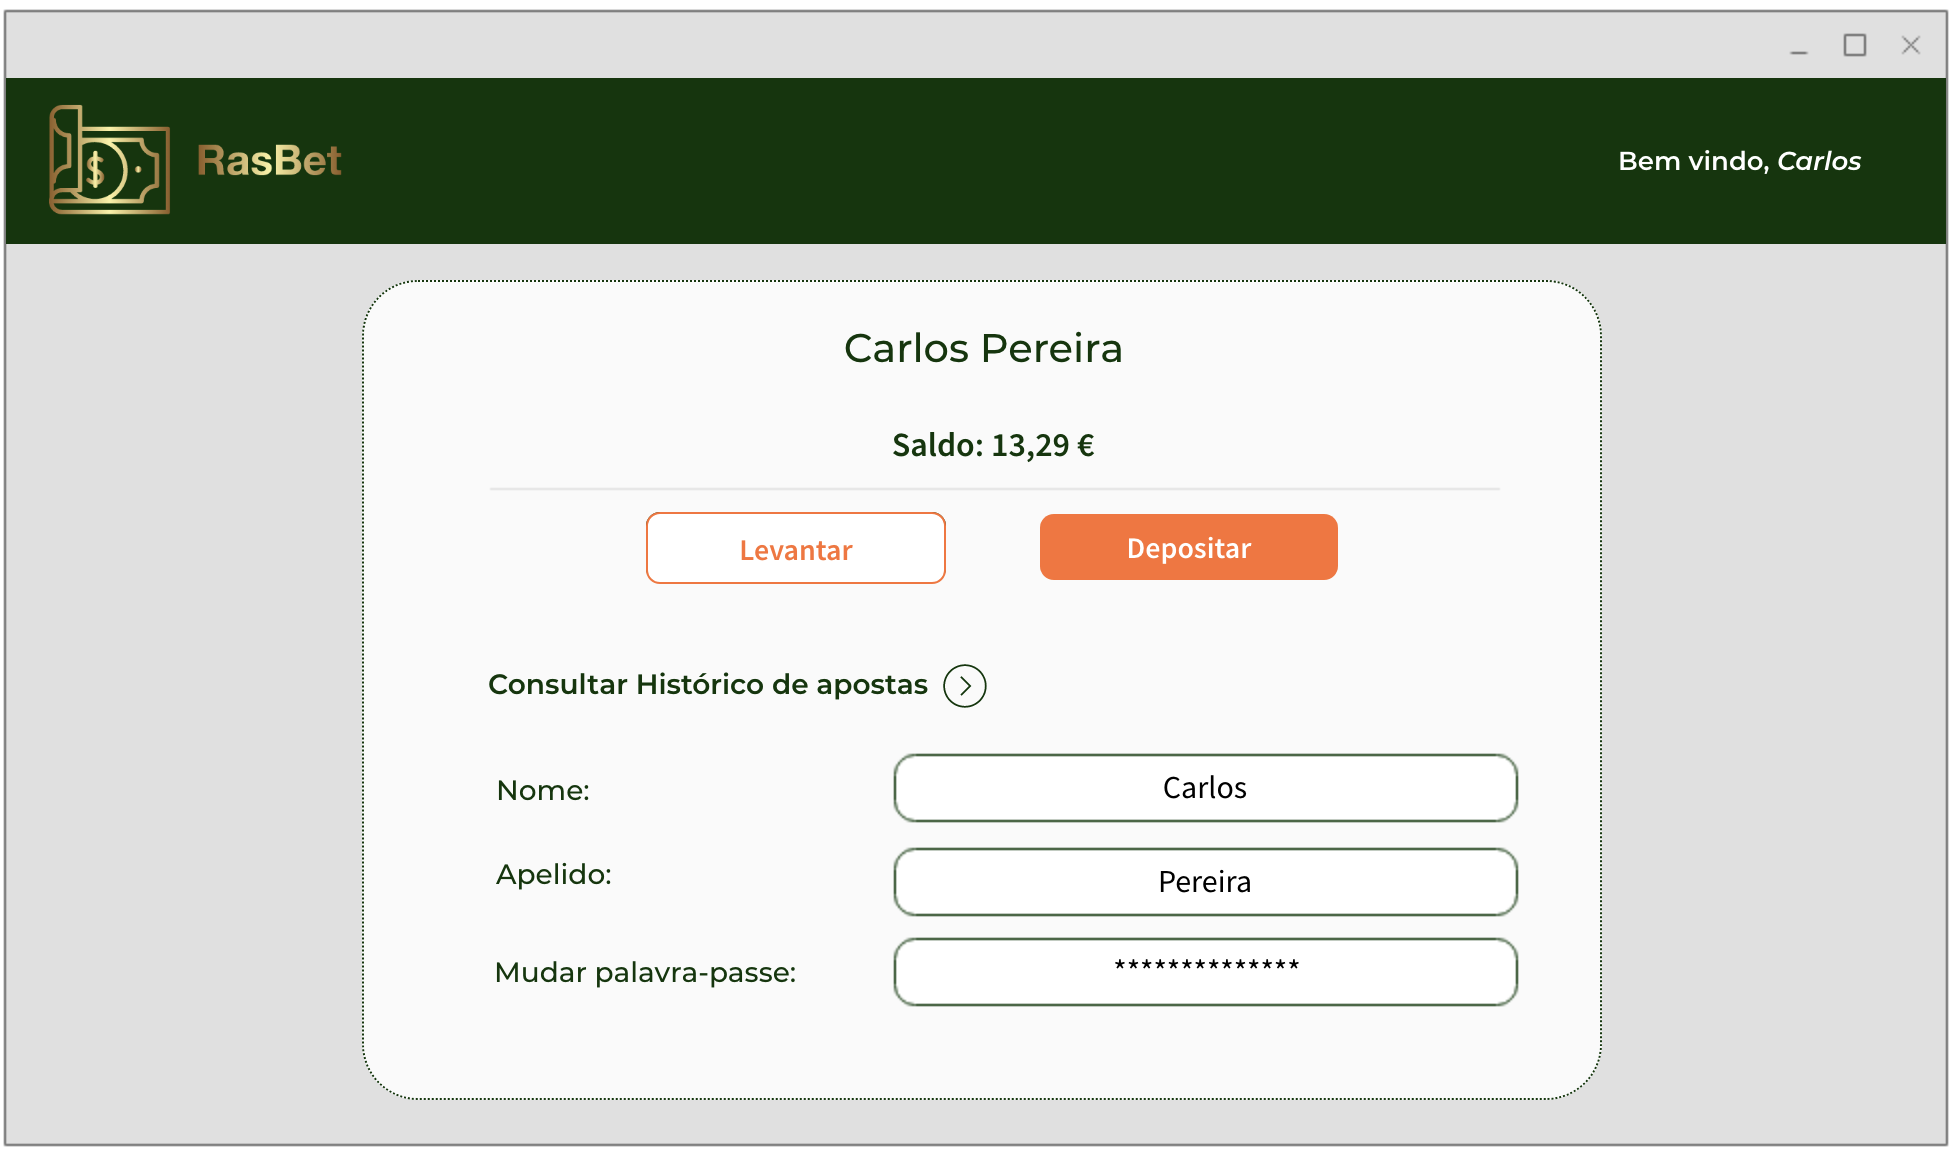
\includegraphics[width=1\textwidth]{imagens/ambitoProduto/Mockups/M_Configuracoes.png}
\caption{Mockup de Alterar informações de perfil}
\end{figure}

\subsection{Consultar jogos}
\begin{figure}[H]
\centering
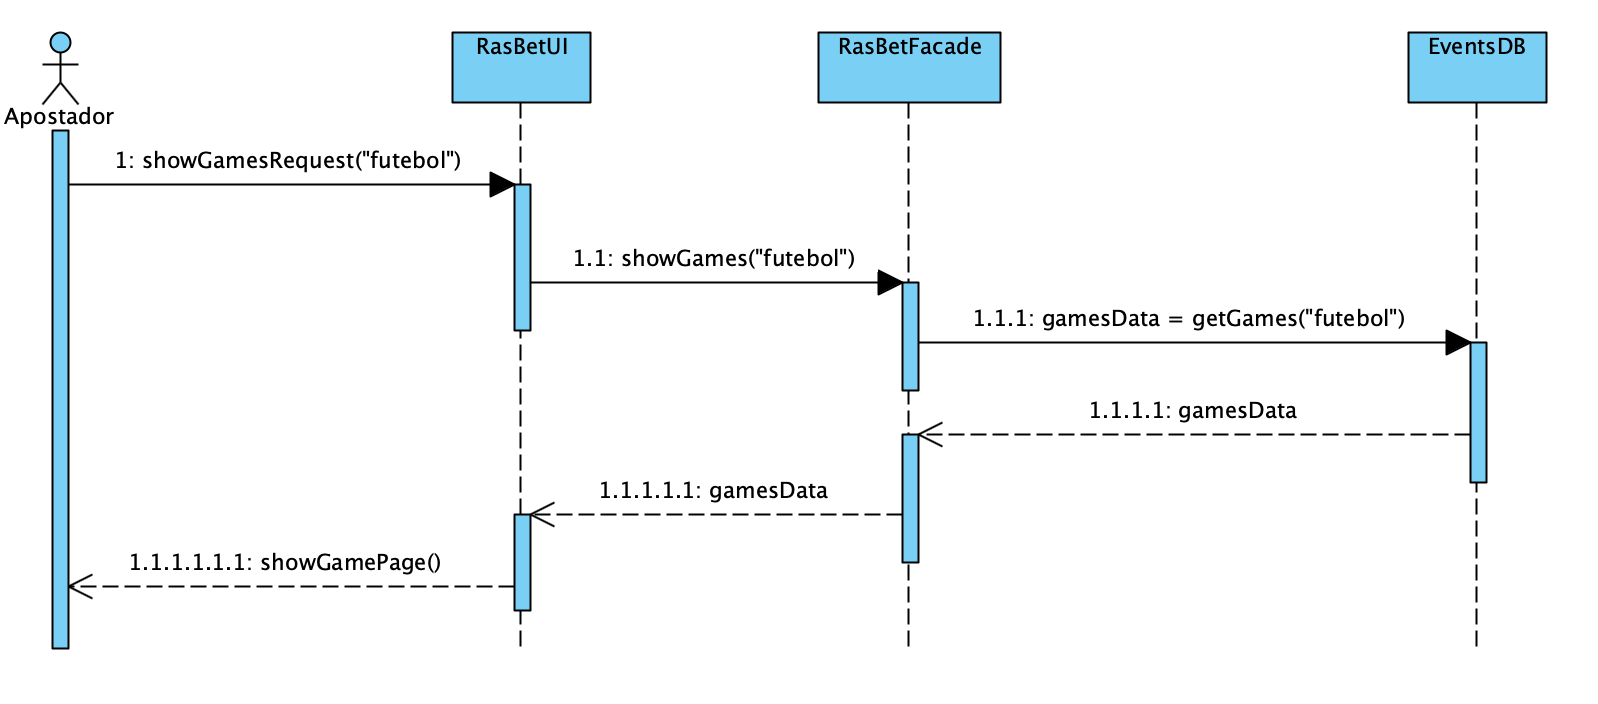
\includegraphics[width=1\textwidth]{imagens/ambitoProduto/SConsultaJogo.png}
\caption{Diagrama de Sequência de Consultar jogos}
\end{figure}
\begin{figure}[H]
\centering
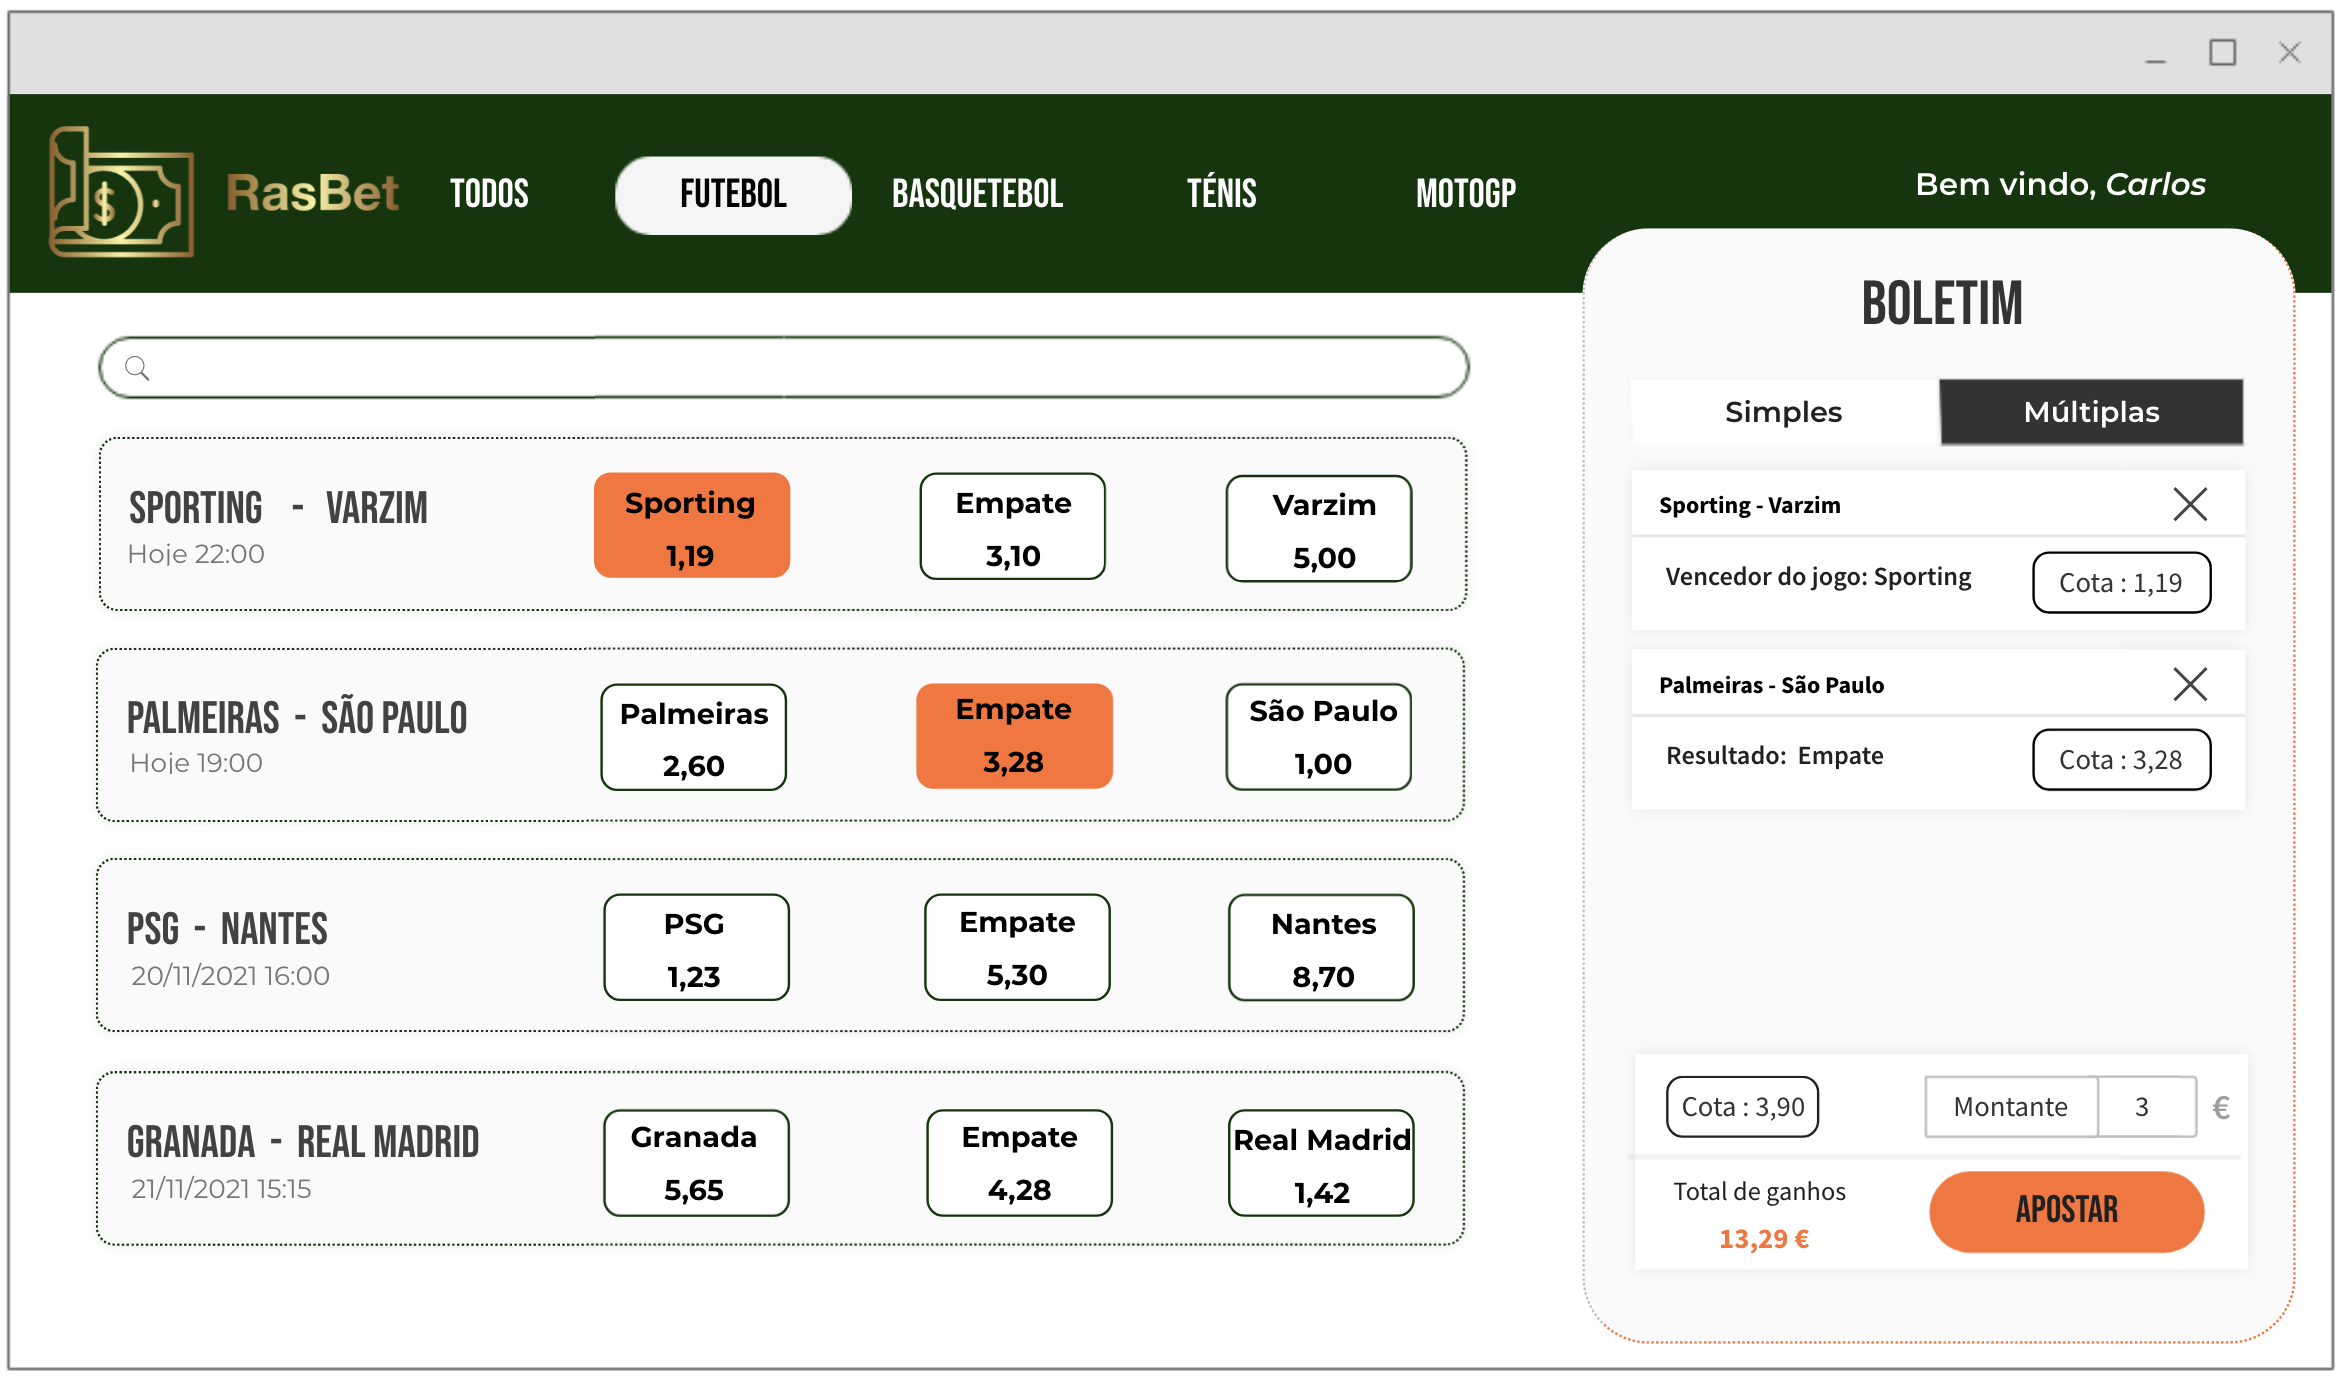
\includegraphics[width=1\textwidth]{imagens/ambitoProduto/Mockups/M_consultarJogos.png}
\caption{Mockup de Consultar jogos}
\end{figure}

\subsection{Fazer Aposta}
\begin{figure}[H]
\centering
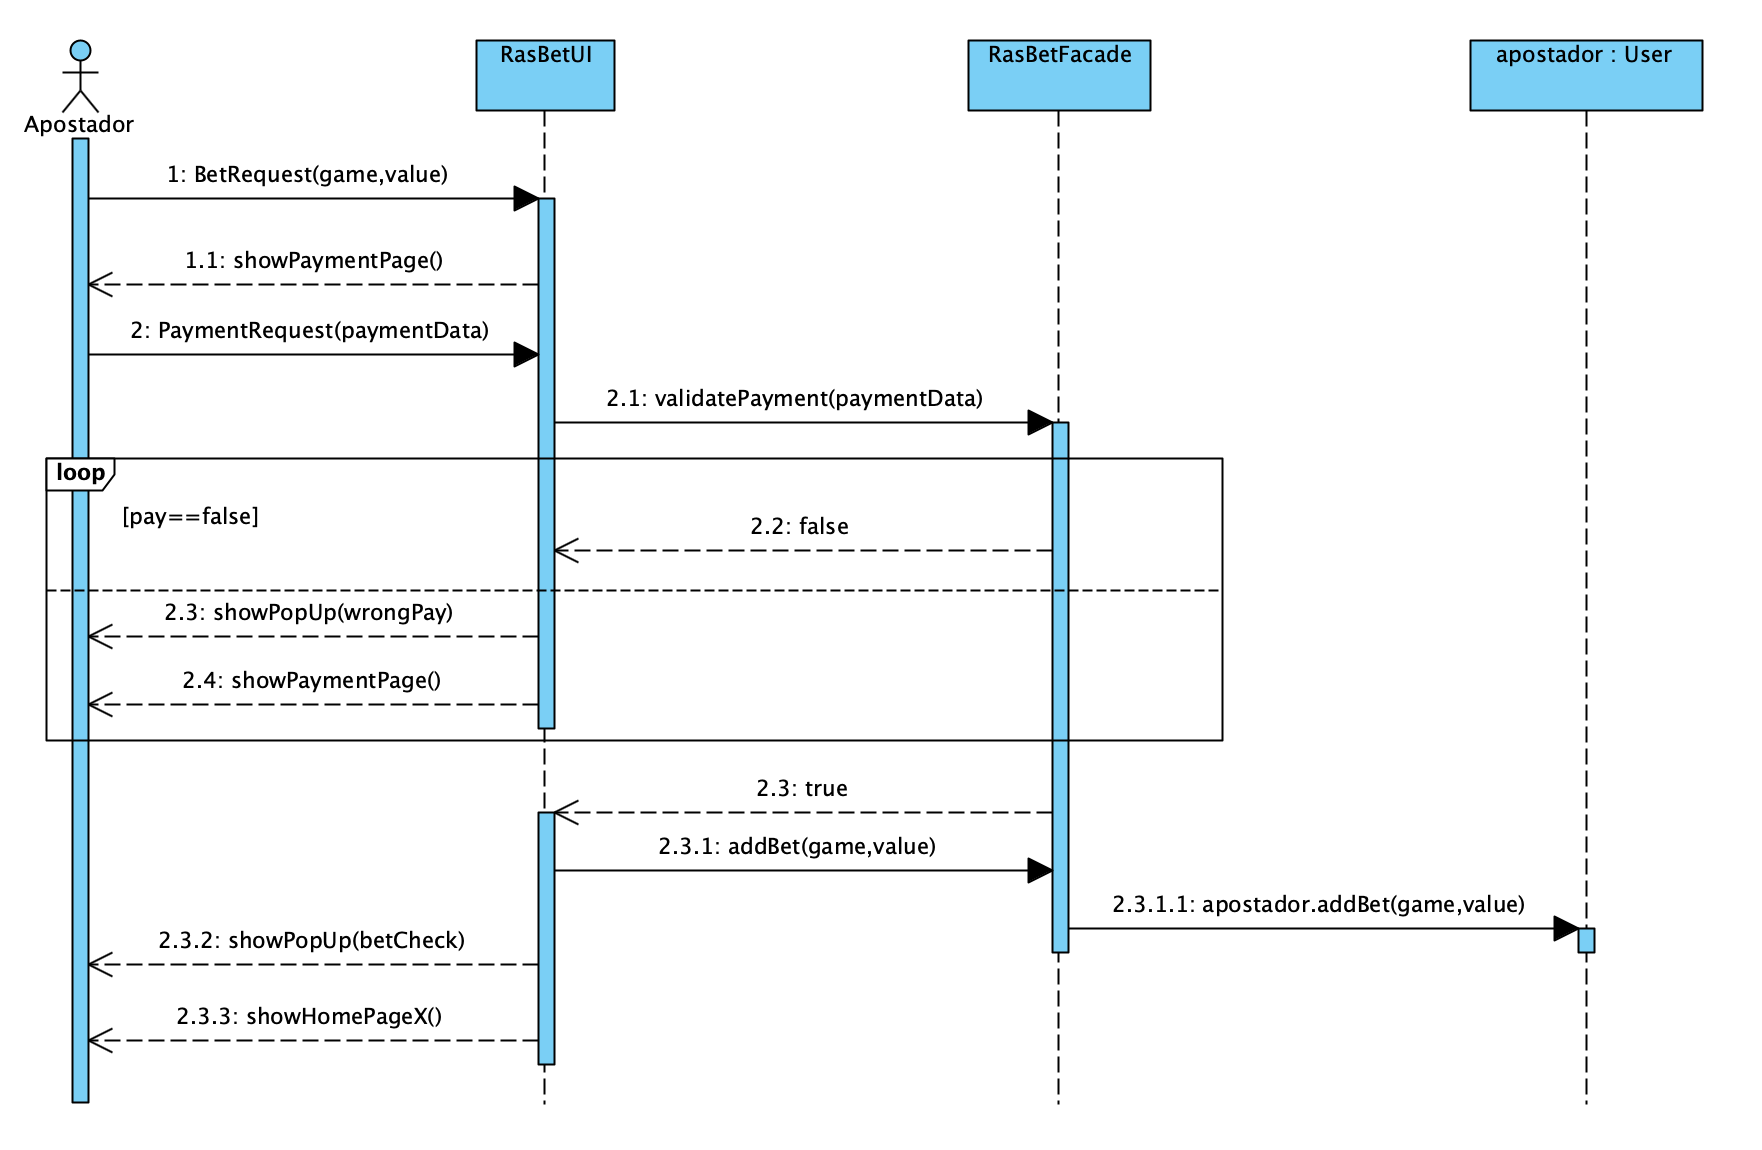
\includegraphics[width=1\textwidth]{imagens/ambitoProduto/SFazerAposta.png}
\caption{Diagrama de Sequência de Consultar jogos}
\end{figure}

\begin{figure}[H]
\centering
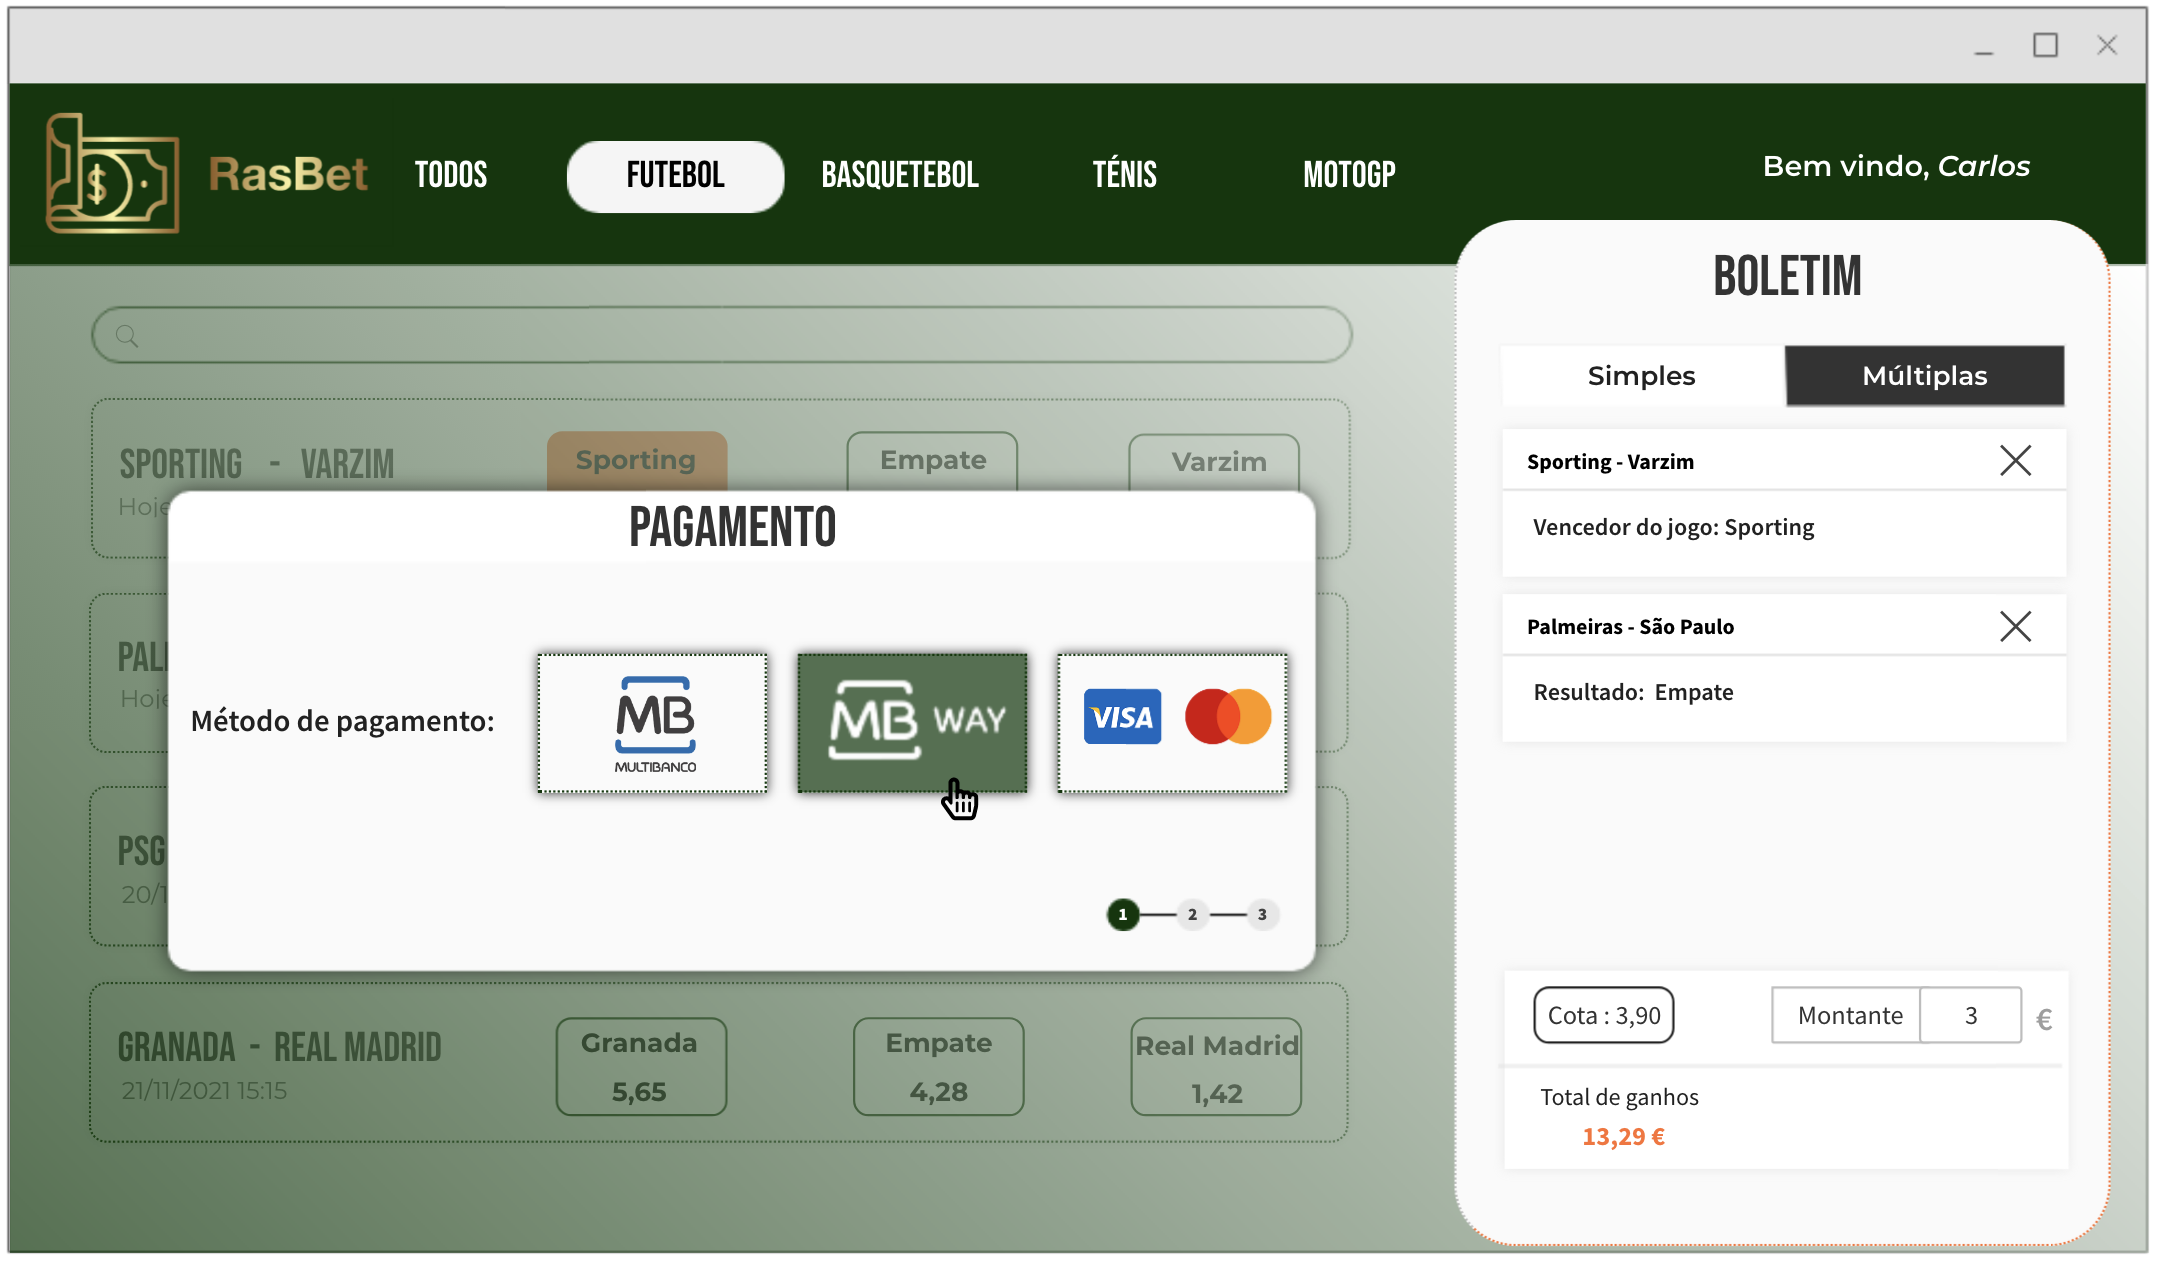
\includegraphics[width=1\textwidth]{imagens/ambitoProduto/Mockups/M_Apostar1.png}
\caption{Mockup de Fazer Aposta 1}
\end{figure}
\begin{figure}[H]
\centering
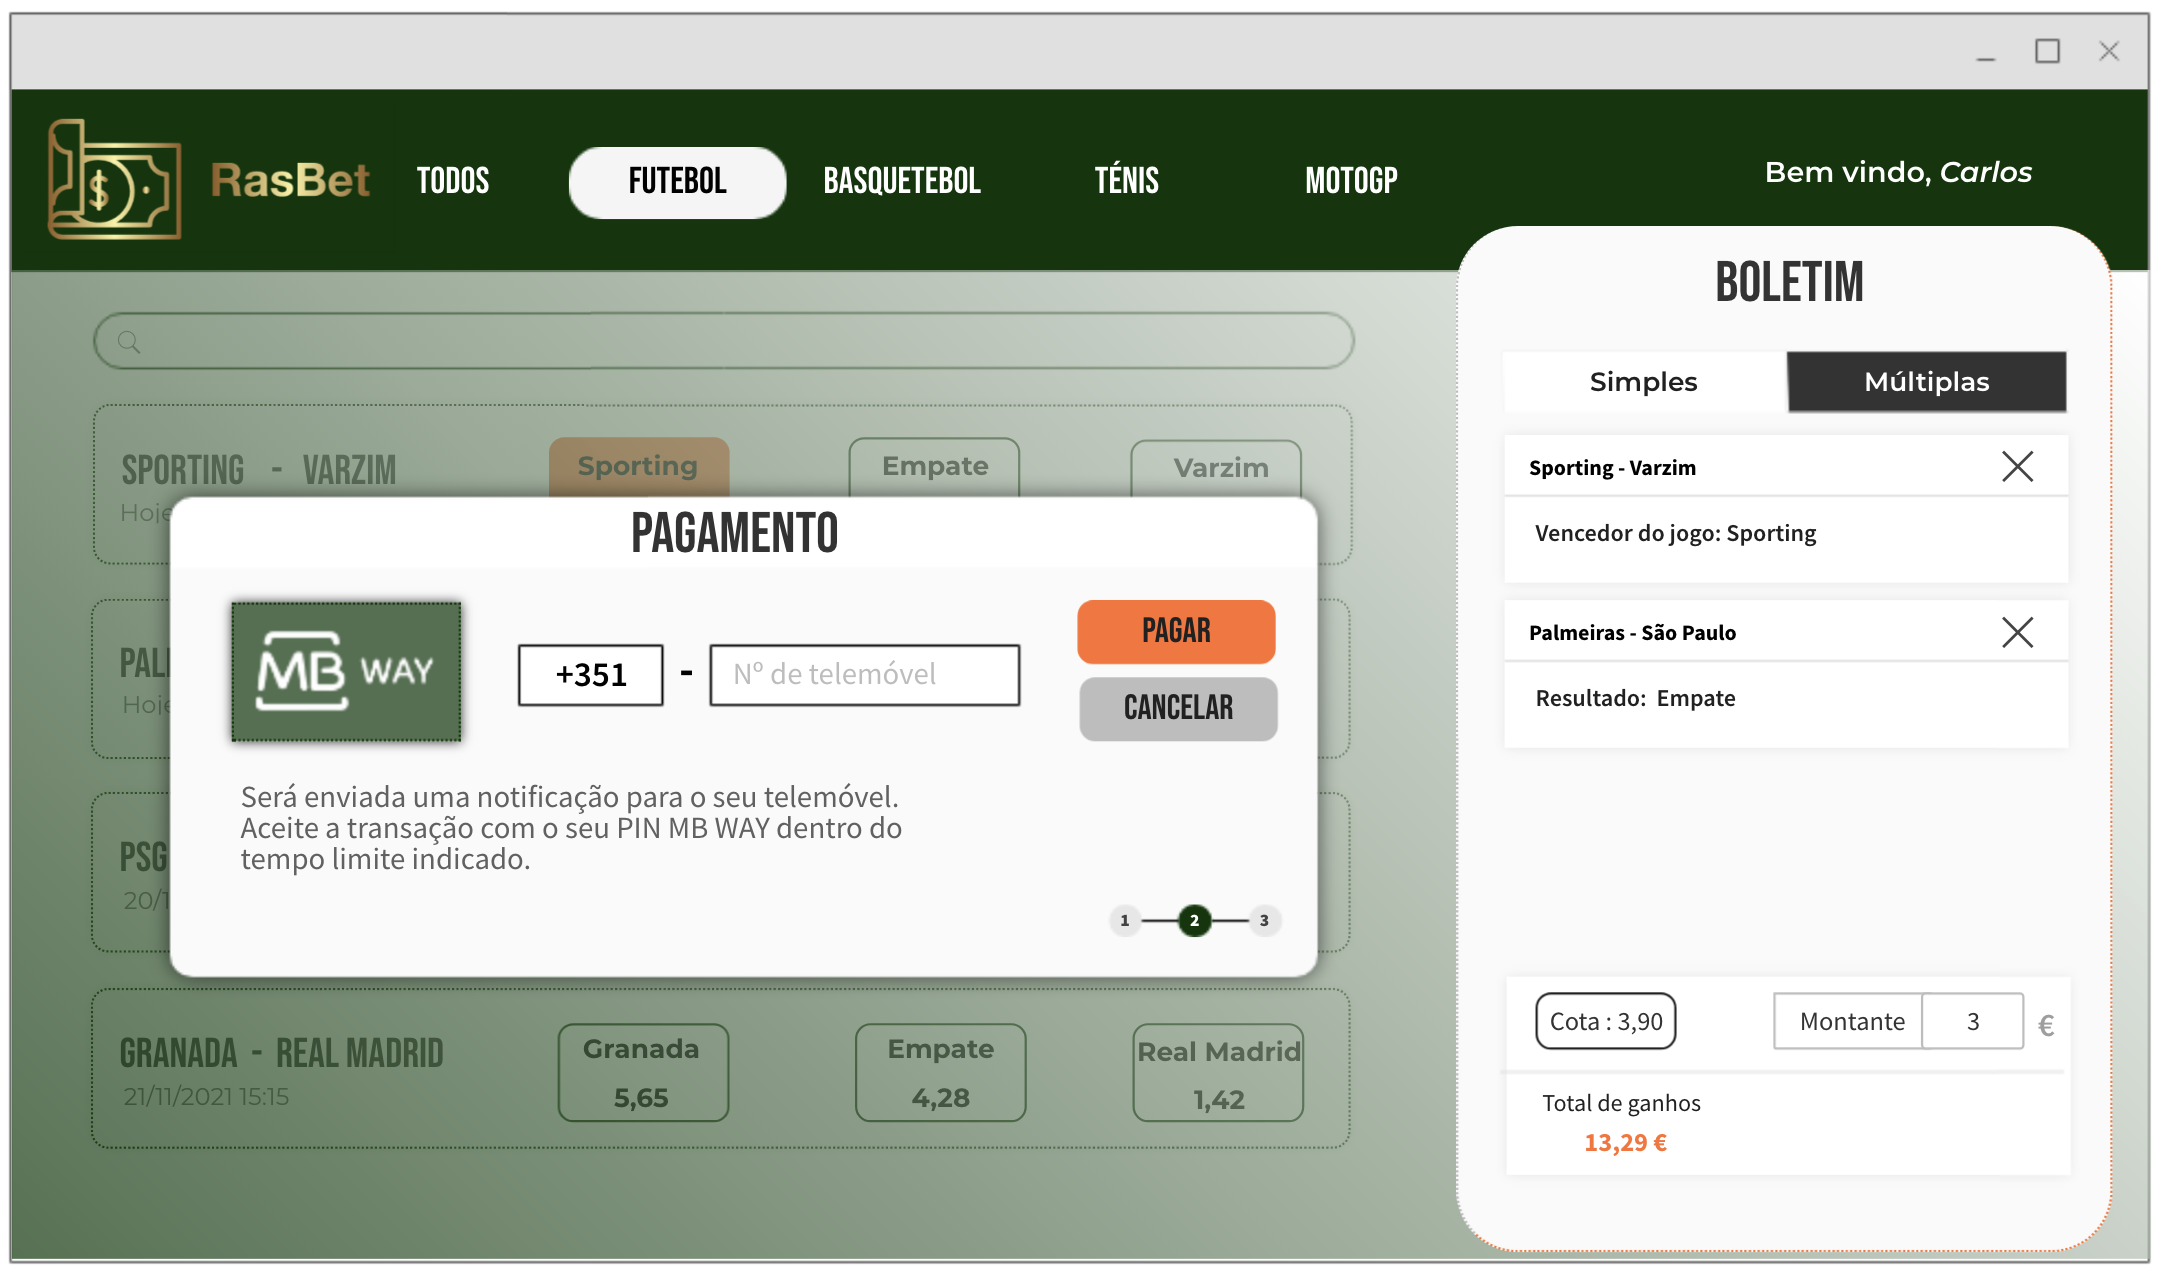
\includegraphics[width=1\textwidth]{imagens/ambitoProduto/Mockups/M_Apostar2.png}
\caption{Mockup de Fazer Aposta 2}
\end{figure}
\begin{figure}[H]
\centering
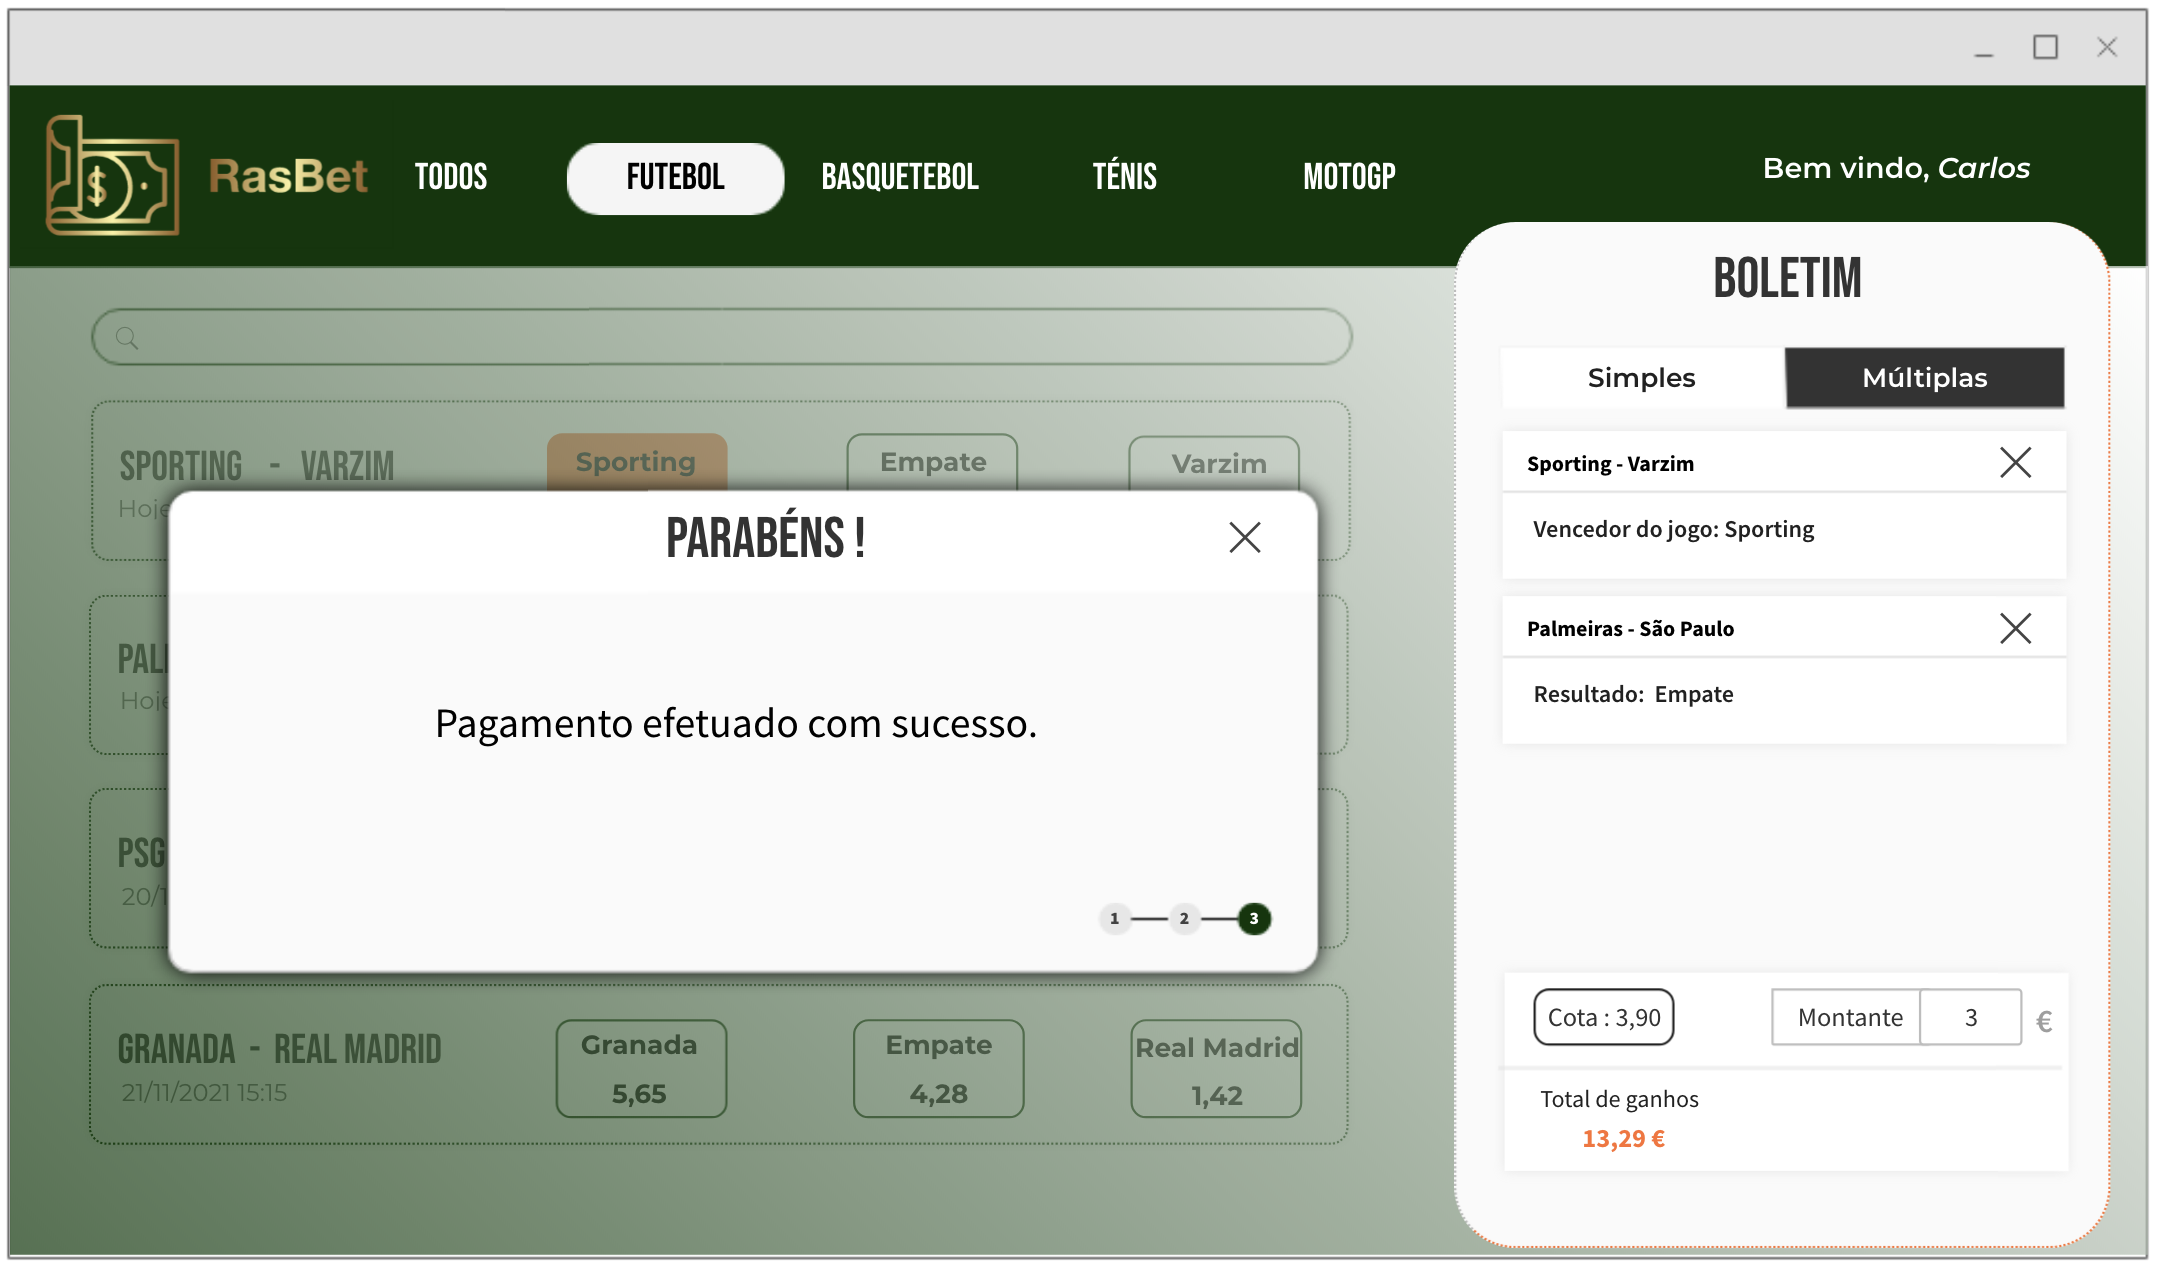
\includegraphics[width=1\textwidth]{imagens/ambitoProduto/Mockups/M_Apostar3.png}
\caption{Mockup de Fazer Aposta 3}
\end{figure}

\subsection{Consultar histórico de Apostas}
\begin{figure}[H]
\centering
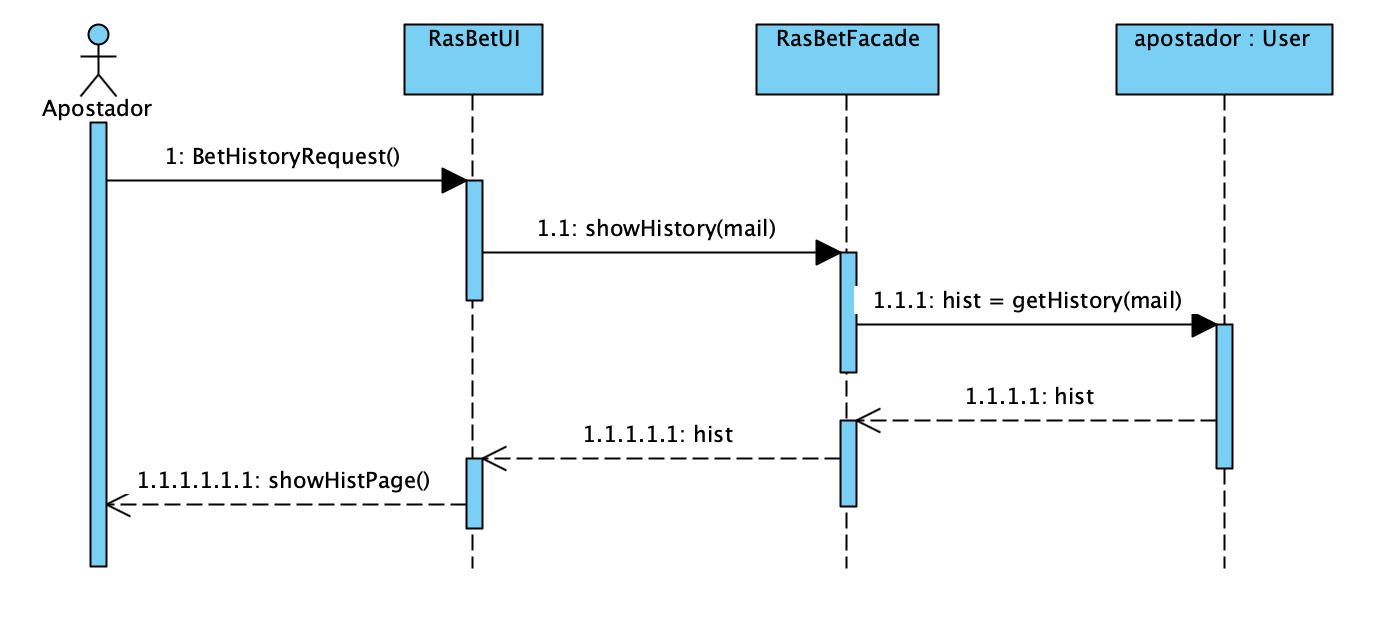
\includegraphics[width=1\textwidth]{imagens/ambitoProduto/SconsultaA.png}
\caption{Diagrama de Sequência de Consultar histórico de Apostas}
\end{figure}
\begin{figure}[H]
\centering
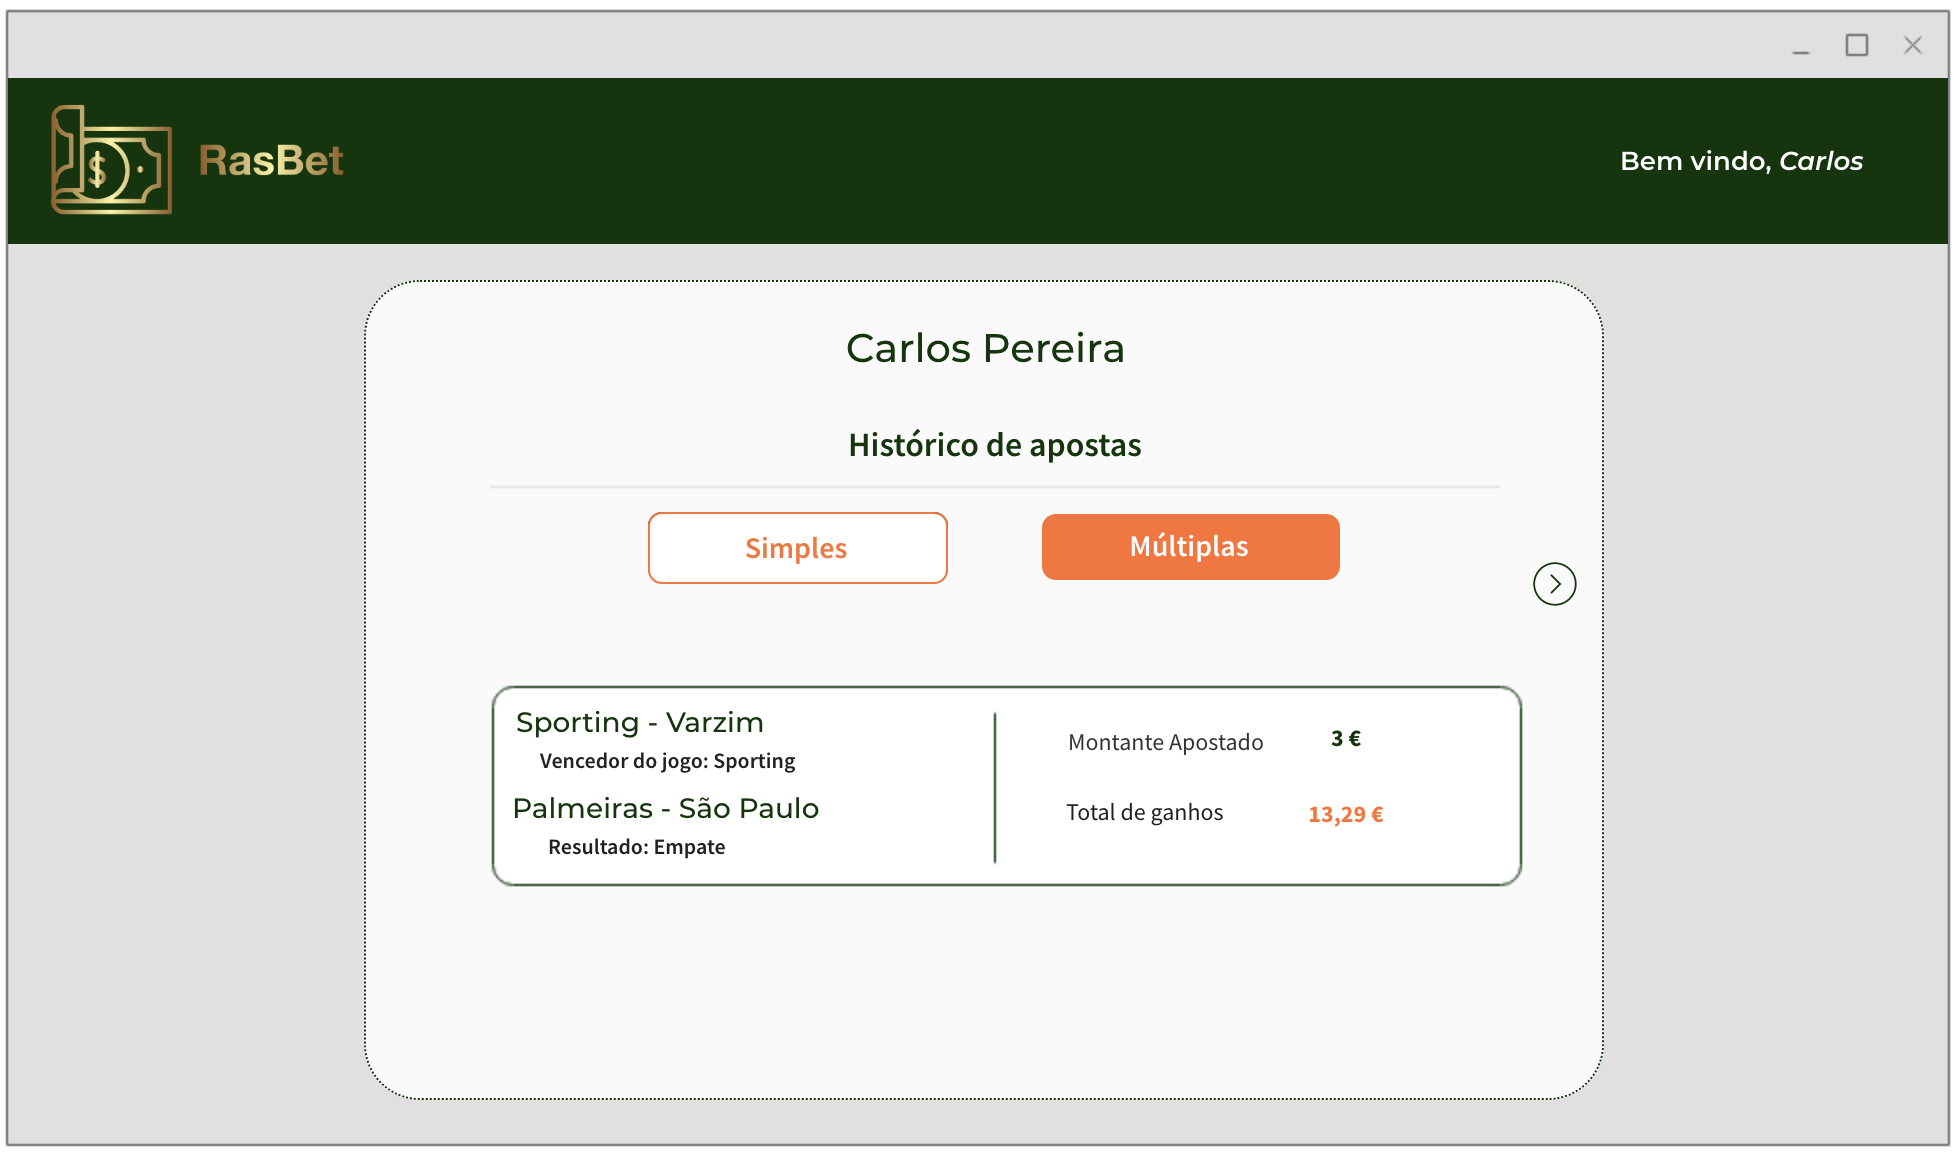
\includegraphics[width=1\textwidth]{imagens/ambitoProduto/Mockups/M_HistoricoApostas.png}
\caption{Mockup de Consultar histórico de Apostas}
\end{figure}

\subsection{Consultar histórico de transações}
\begin{figure}[H]
\centering
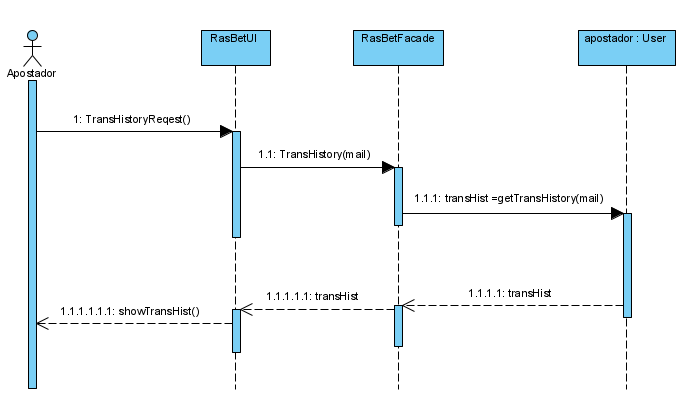
\includegraphics[width=1\textwidth]{imagens/ambitoProduto/STransHistory.png}
\caption{Diagrama de Sequência de Consultar histórico de transações}
\end{figure}
\begin{figure}[H]
\centering
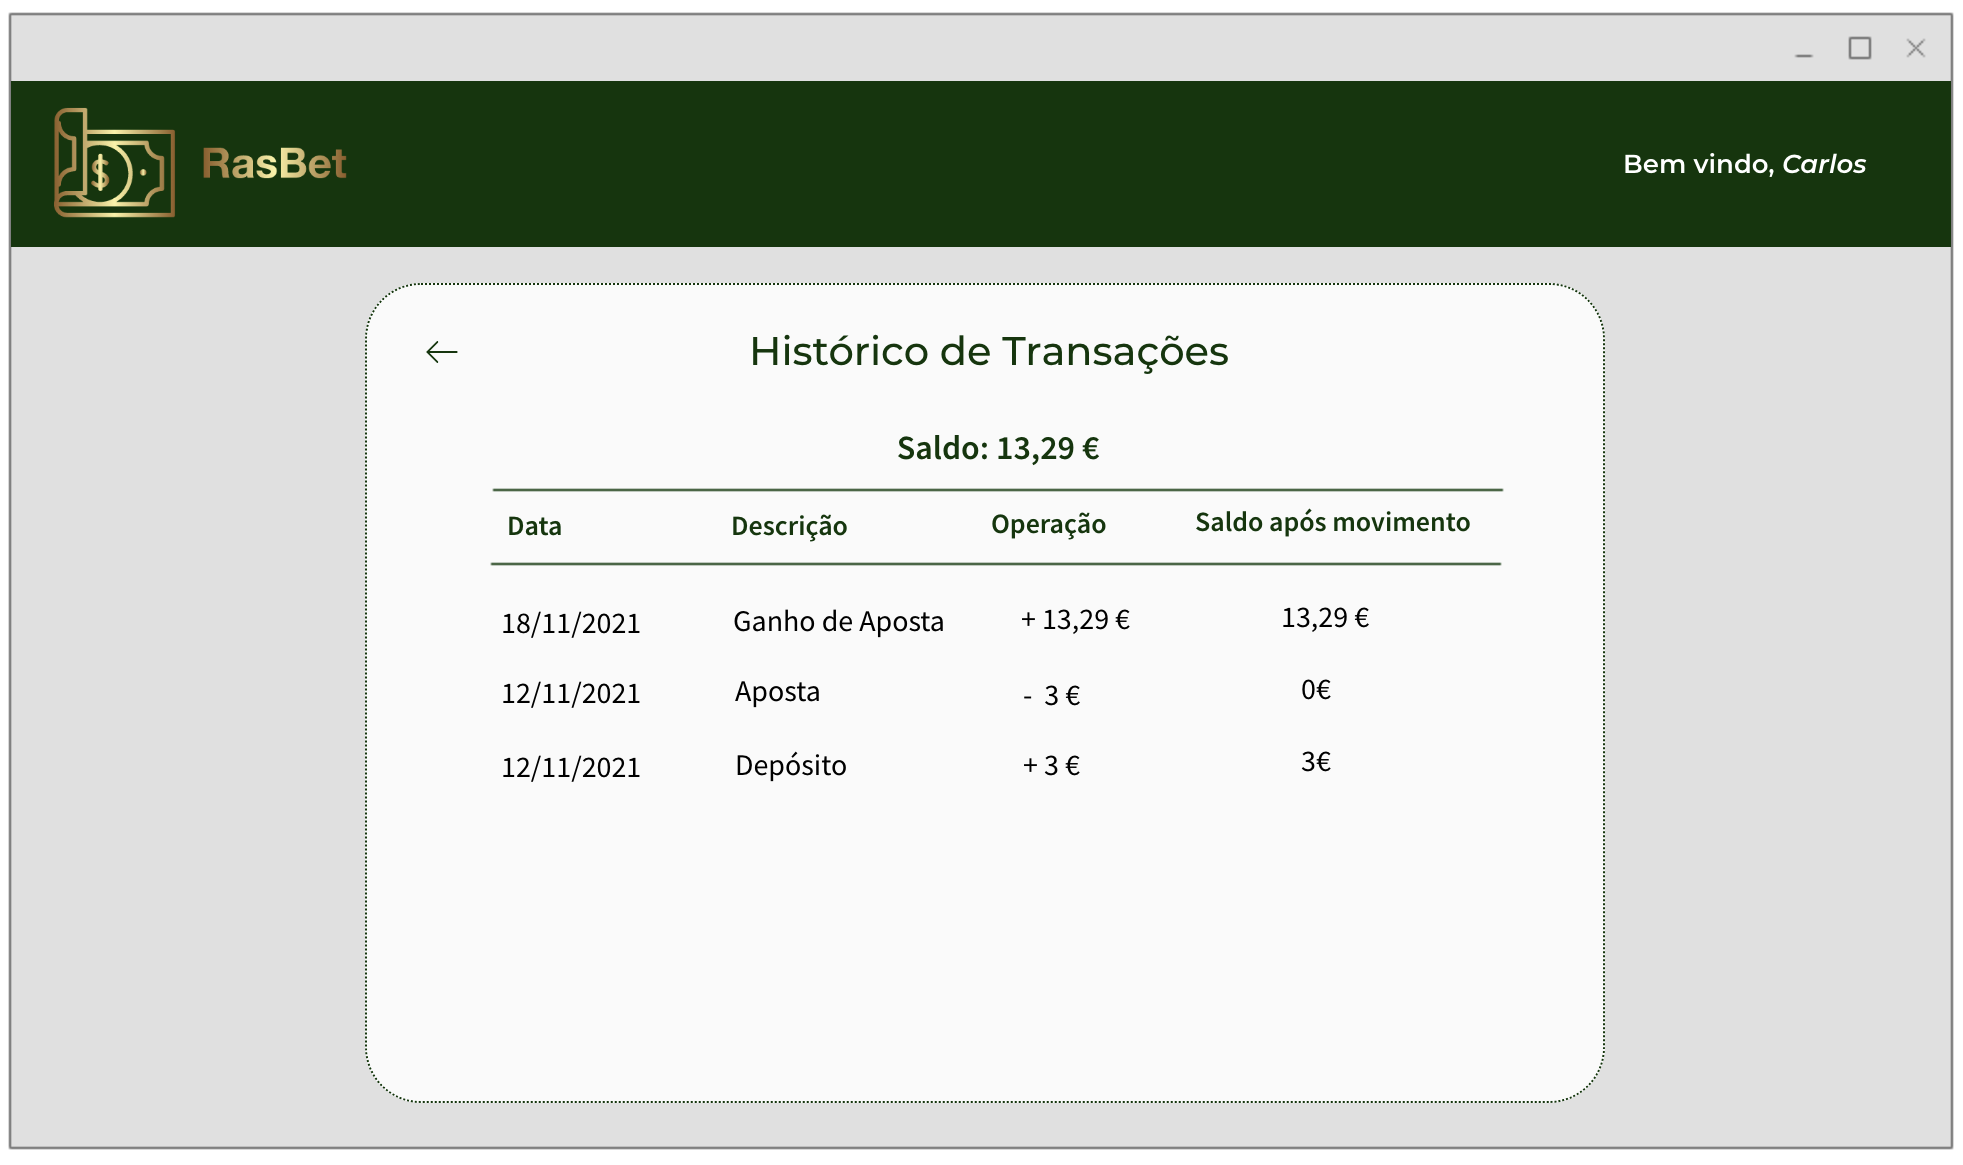
\includegraphics[width=1\textwidth]{imagens/ambitoProduto/Mockups/M_histTransacoes.png}
\caption{Mockup de Consultar histórico de Transações}
\end{figure}

\subsection{Depositar/Levantar dinheiro}
\begin{figure}[H]
\centering
\includegraphics[width=1\textwidth]{imagens/ambitoProduto/S_depositar:levantar.png}
\caption{Diagrama de Sequência de Depositar/Levantar dinheiro}
\end{figure}

\subsection{Inserir Odd}
\begin{figure}[H]
\centering
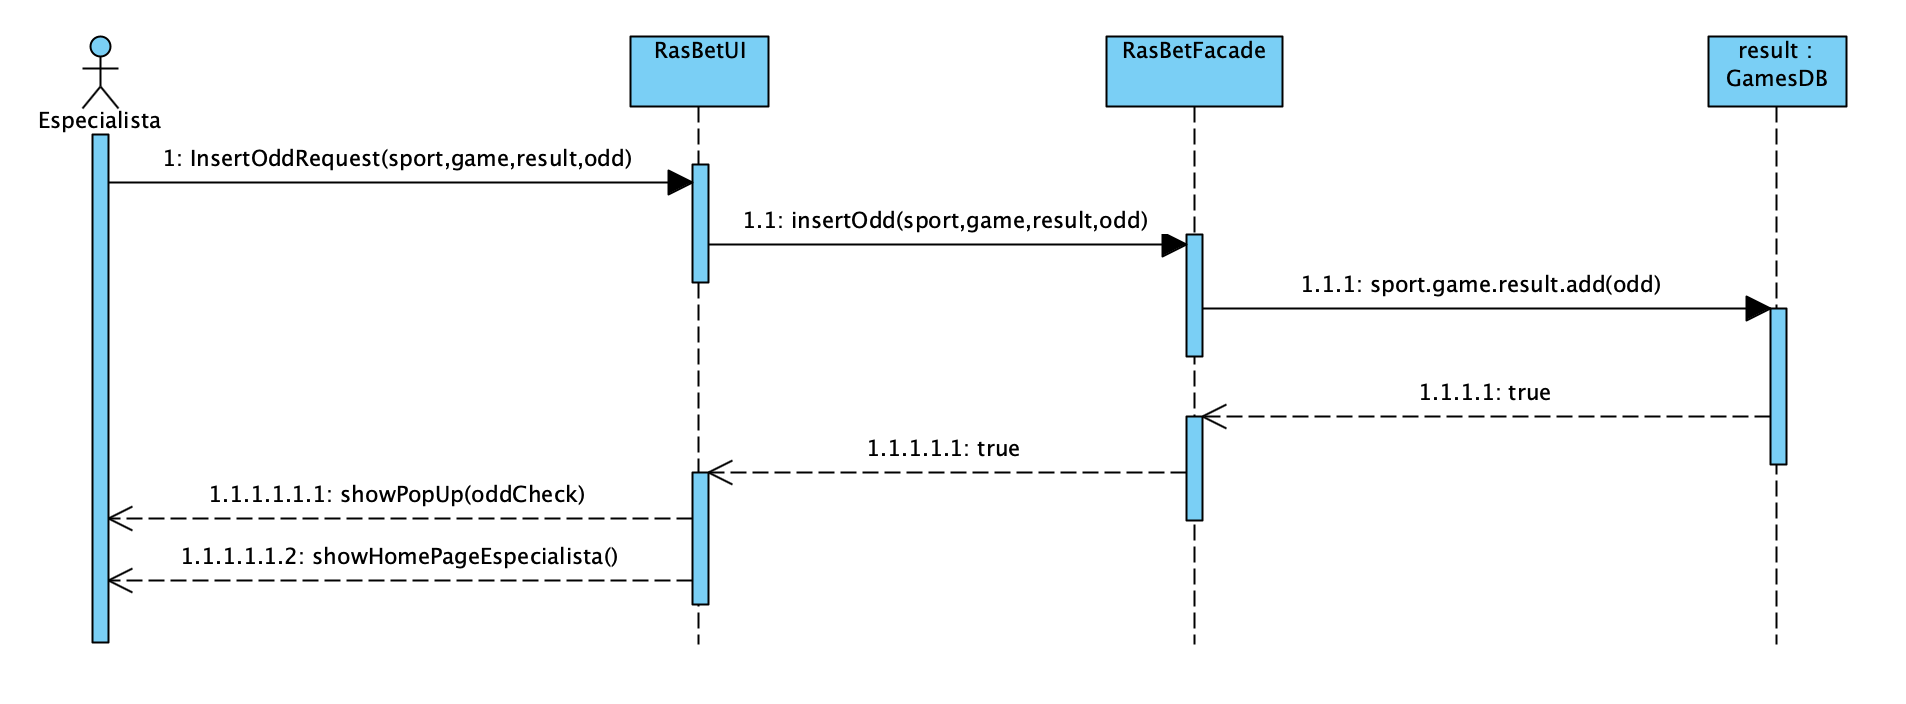
\includegraphics[width=1\textwidth]{imagens/ambitoProduto/SInserirOdd.png}
\caption{Diagrama de Sequência de Inserir Odd}
\end{figure}
\begin{figure}[H]
\centering
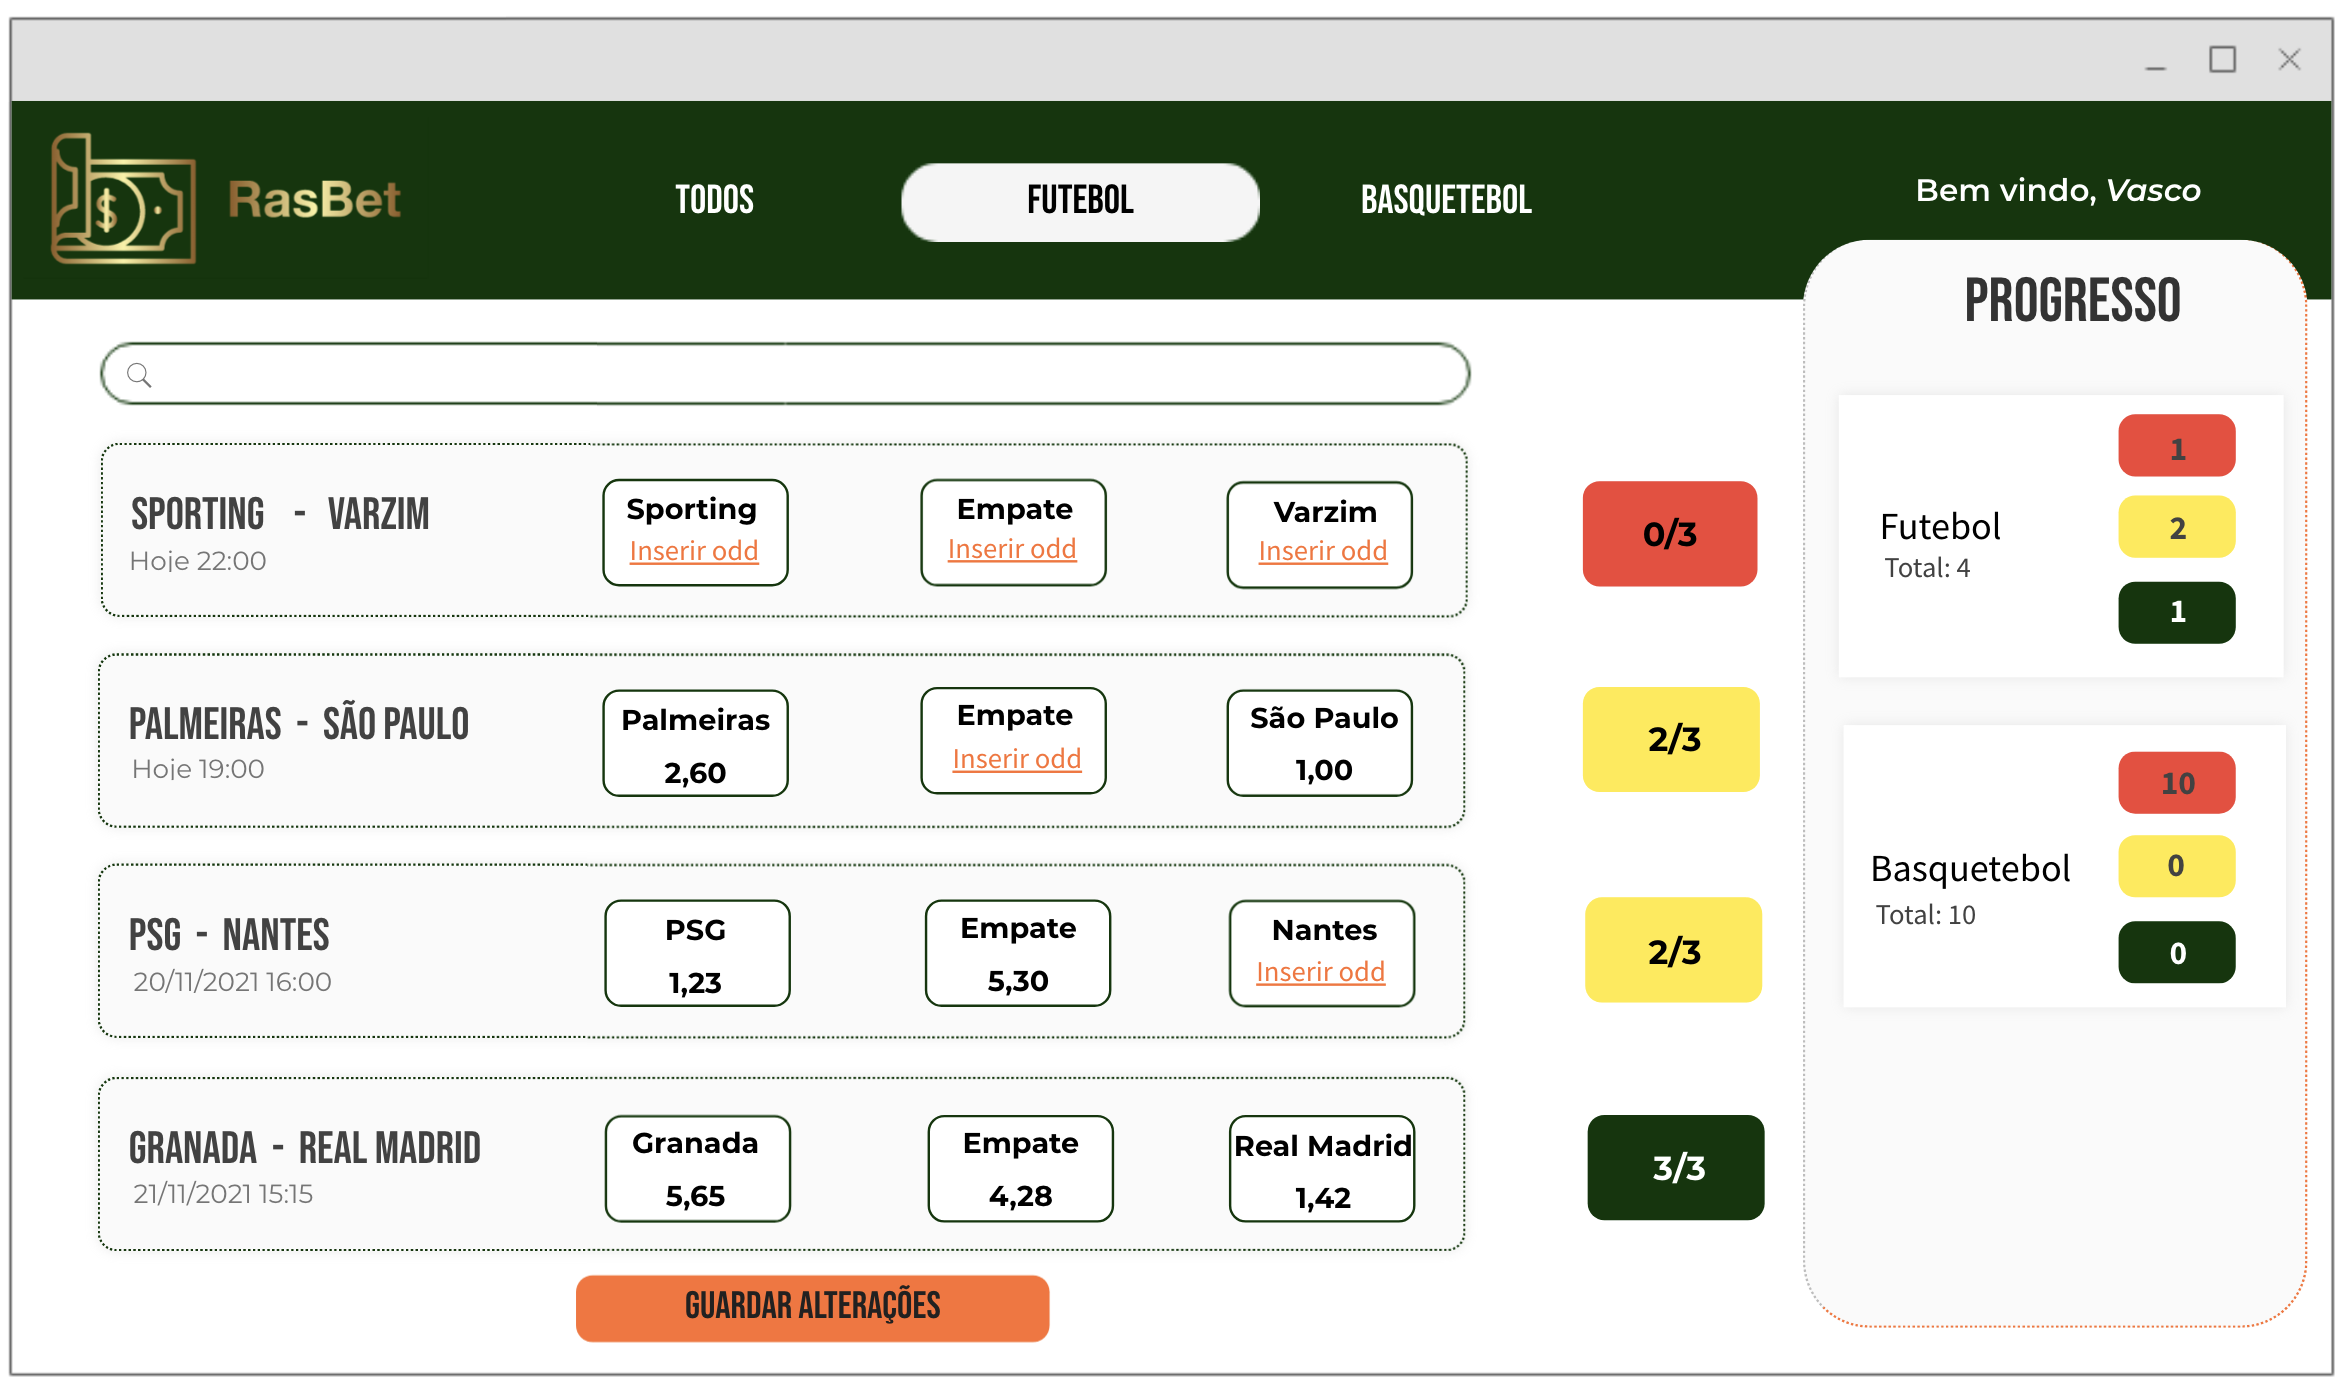
\includegraphics[width=1\textwidth]{imagens/ambitoProduto/Mockups/M_InserirODD.png}
\caption{Mockup de Inserir Odd}
\end{figure}

\subsection{Alterar e suspender jogos}
\begin{figure}[H]
\centering
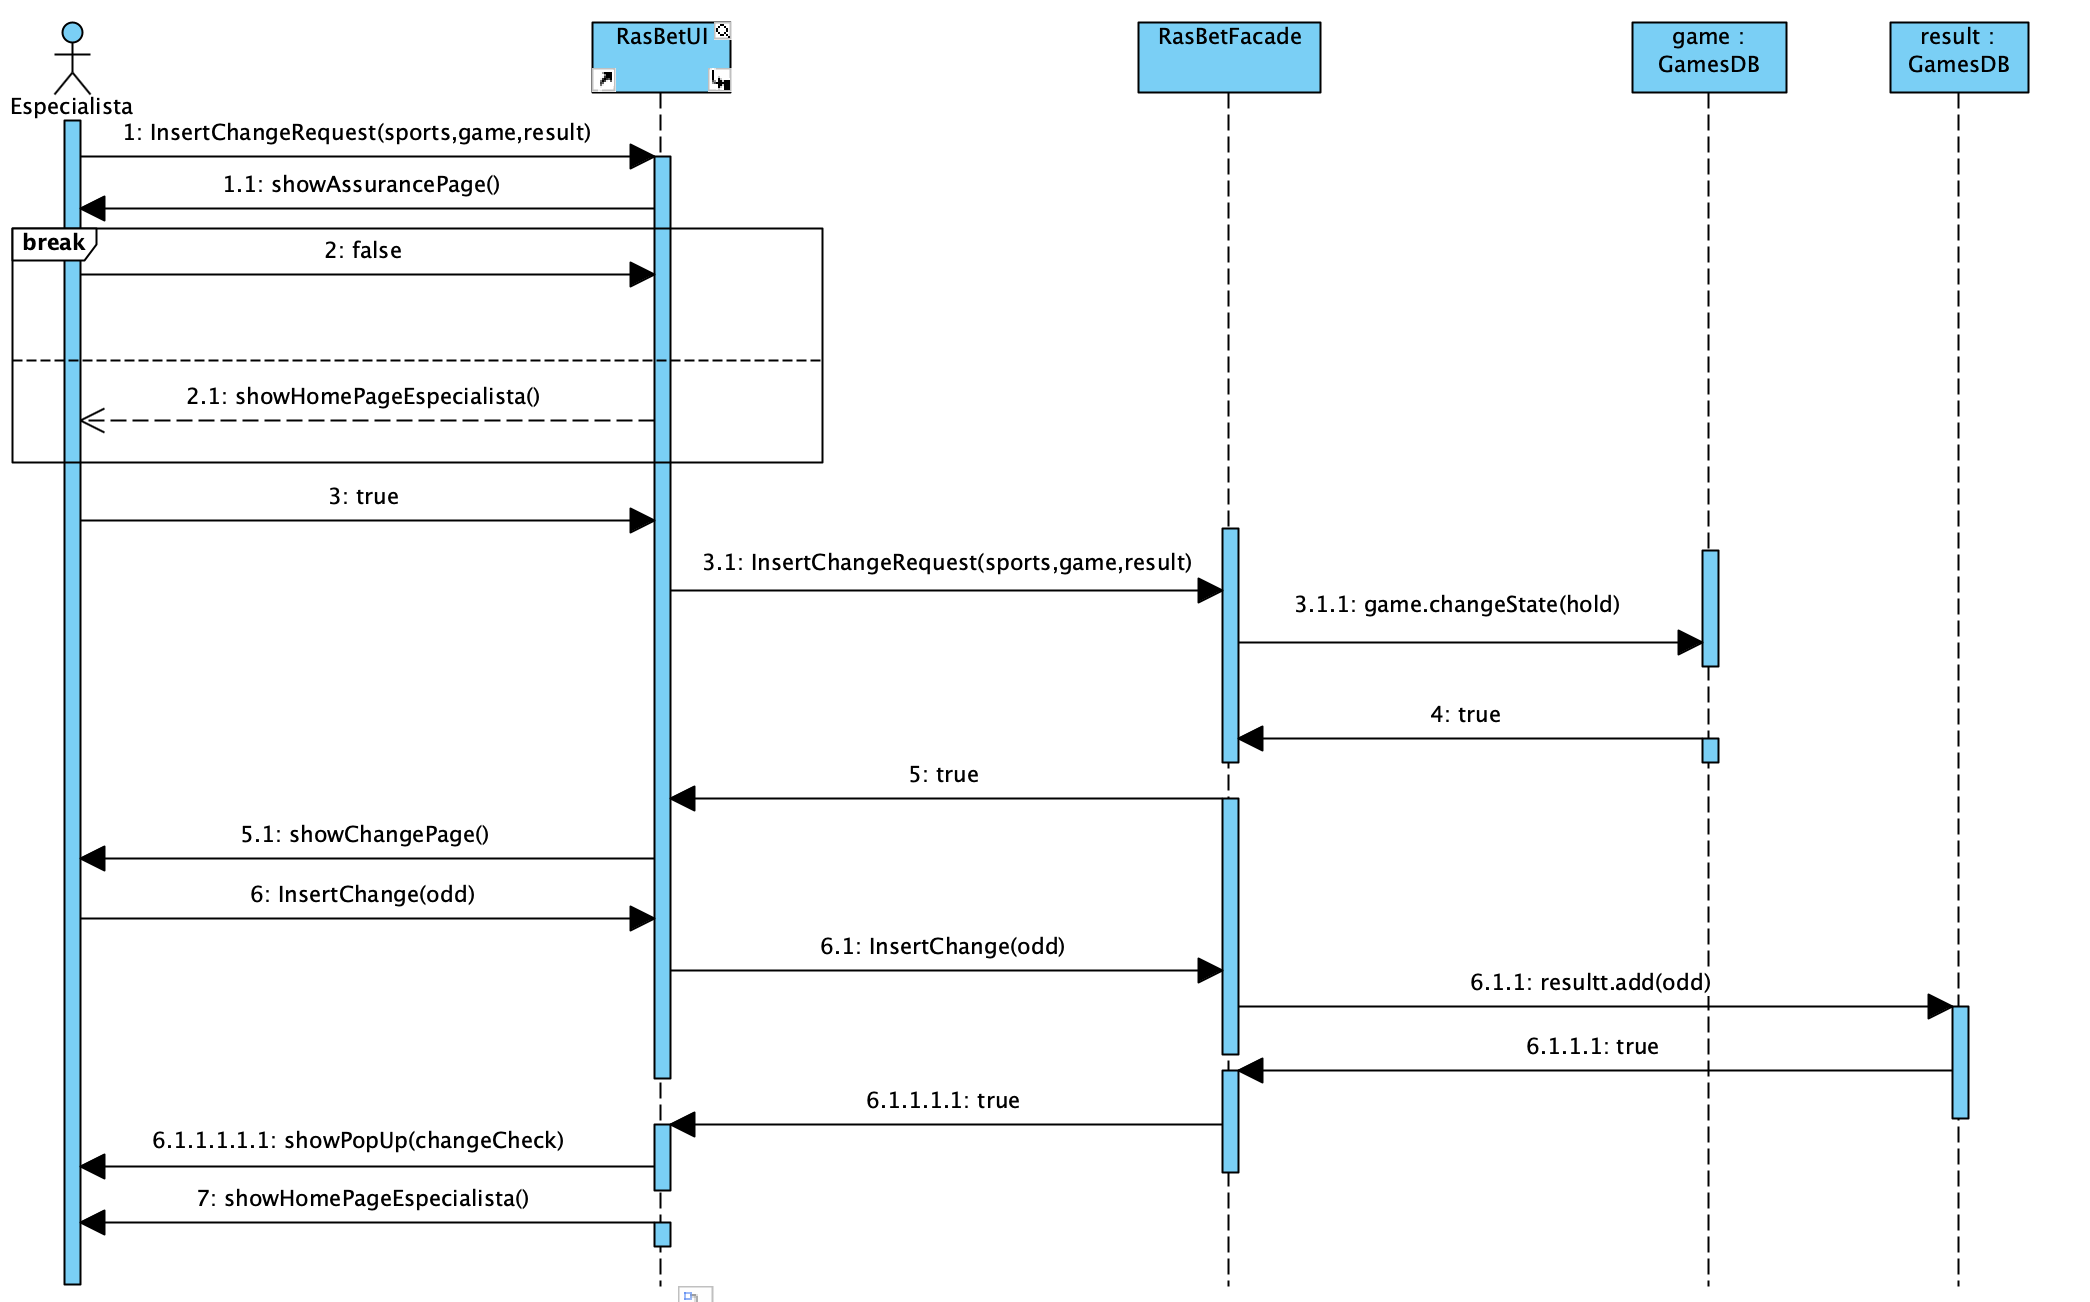
\includegraphics[width=1\textwidth]{imagens/ambitoProduto/S_alterar.png}
\caption{Diagrama de Sequência de Alterar e suspender jogos}
\end{figure}
\begin{figure}[H]
\centering
\includegraphics[width=1\textwidth]{imagens/ambitoProduto/Mockups/M_Altera:sus1.png}
\caption{Mockup de Alterar e suspender jogos 1}
\end{figure}
\begin{figure}[H]
\centering
\includegraphics[width=1\textwidth]{imagens/ambitoProduto/Mockups/M_Altera:sus2.png}
\caption{Mockup de Alterar e suspender jogos 2}
\end{figure}
\begin{figure}[H]
\centering
\includegraphics[width=1\textwidth]{imagens/ambitoProduto/Mockups/M_Altera:sus3.png}
\caption{Mockup de Alterar e suspender jogos 3}
\end{figure}
\chapter{Requisitos Funcionais}
% Usar para a contagem dos requisitos

\section{Modelação de Requisitos}
Para o levantamento de requisitos, foi utilizado como forma de representação, a \textit{requirement shell} do modelo de \textit{Volere}, de forma a descrever concisamente os requisitos.

\begin{table}[H]
\centering
\begin{tabular}{|lll|} 
\hline
\textbf{Requirement}         & \textbf{Type}:         &           \\ 
\hline
\multicolumn{3}{|p{14.5cm}|}{\textbf{Description:}}    \\
\hline
\multicolumn{3}{|p{14.5cm}|}{\textbf{Rationale:} }      \\
\hline
\multicolumn{3}{|p{14.5cm}|}{\textbf{Originator:}}                                              \\ 
\hline
\multicolumn{3}{|p{14.5cm}|}{\textbf{Fit Criterion:} }                                              \\ 
\hline
\textbf{Customer Satisfaction:}  & \textbf{Customer Dissatisfaction:}  & \textbf{Priority:}               \\ 
\hline
\multicolumn{3}{|l|}{\textbf{Conflicts:}}                                                      \\
\hline
\multicolumn{3}{|l|}{\textbf{History:}} 
\\\hline
\end{tabular}
\caption{Exemplo especificação de Requisitos}
\end{table}

Como caracterização da tabela de representação de requisitos, é necessário descrever os campos:
\begin{itemize}
    \item \textbf{Requirement:} Número de identificação do requisito.
    \item \textbf{Requirement Type:} Tipo de requisito, considerando o modelo de \textit{Volere} (Requisito Funcional 9).
    \item \textbf{Event/Use Case:} Número do evento ou Use Case associado.
    \item \textbf{Description:} Descrição, clara e concisa do requisito.
    \item \textbf{Rationale:} Justificação, razão da existência do requisito.
    \item \textbf{Originator:} Quem originou o requisito.
    \item \textbf{Fit Criterion:} Critério em que se insere.
    \item \textbf{Customer Satisfaction:} Apreciação de 1 a 5 em que 1 significa que existe um interesse pequeno que o requisito seja satisfeito, e 5 significa que irão ficar extremamente satisfeitos com a implementação do requisito.
    \item \textbf{Customer Dissatisfaction:} Apreciação de 1 a 5 em que 1 significa que é quase irrelevante que o requisito seja satisfeito, e 5 significa que irão ficar extremamente insatisfeitos com a ausência da correcta implementação do requisito.
    \item \textbf{Priority:} Define o índice de prioridade de implementação de requisitos:
    \begin{itemize}
        \item \textbf{\color{red}Must}: Requisitos obrigatórios.
        \item \textbf{\color{orange}Should}: Requisitos que devem ser implementados.
        \item \textbf{\color{blue}Could}: Requisitos que não são necessários, mas são desejados.
        \item \textbf{\color{OliveGreen}Won't}: Requisitos que podem ser considerados posteriormente.
    \end{itemize}
    \item \textbf{Conflicts:} Problema encontrado na conceptualização do requisito.
    \item \textbf{History:} Data de criação do requisito.
\end{itemize}

\begin{comment}
Vou por alguns requisitos que me lembre aqui, para fazer-mos reverse engeniring para a entrevista e etc (Não sao obrigatoriamente funcionais, é so um rascunho),
qualquer coisa que discordem mudem!!
\end{comment}

\section{Requisitos sobre Utilizadores}

\newcounter{reqnum}
\setcounter{reqnum}{1}
%REQ1%
\begin{table}[H]
\centering
\begin{tabular}{|lll|} 
\hline
\textbf{Requirement:} \#\thereqnum  & \textbf{Type}: 9        &           \\ 
\hline
\multicolumn{3}{|p{14.5cm}|}{\textbf{Description:} O Apostador tem de se registar na aplicação para a poder utilizar.}    \\
\hline
\multicolumn{3}{|p{14.5cm}|}{\textbf{Rationale:} Garantir controlo de acesso.}      \\
\hline
\multicolumn{3}{|p{14.5cm}|}{\textbf{Originator:} Introspecção}                                              \\ 
\hline
\multicolumn{3}{|p{14.5cm}|}{\textbf{Fit Criterion:} O apostador fica registado na base de dados}                                           \\ 
\hline
\textbf{Customer Satisfaction:} 2 & \textbf{Customer Dissatisfaction:} 5  & \textbf{Priority: \color{red} Must}               \\ 
\hline
\multicolumn{3}{|l|}{\textbf{Conflicts:} Nenhum}                                                      \\
\hline
\multicolumn{3}{|l|}{\textbf{History:} 9/11/2021} 
\\\hline
\end{tabular}
\caption{Requisito funcional \thereqnum.}
\end{table}
\addtocounter{reqnum}{1}





%REQ2%
\begin{table}[H]
\centering
\begin{tabular}{|lll|} 
\hline
\textbf{Requirement} \#\thereqnum         & \textbf{Type}: 9        &           \\ 
\hline
\multicolumn{3}{|p{14.5cm}|}{\textbf{Description:} O Utilizador edita o seu perfil.}    \\
\hline
\multicolumn{3}{|p{14.5cm}|}{\textbf{Rationale:} Melhorar a sua caracterização pessoal, actualizar informação.}      \\
\hline
\multicolumn{3}{|p{14.5cm}|}{\textbf{Originator:} Joana Melo (Persona)}                                              \\ 
\hline
\multicolumn{3}{|p{14.5cm}|}{\textbf{Fit Criterion:} Os dados são corretamente modificados, e guardados na abse de dados.}                                           \\ 
\hline
\textbf{Customer Satisfaction:} 2  & \textbf{Customer Dissatisfaction:} 5  & \textbf{Priority: \color{orange} Should}               \\ 
\hline
\multicolumn{3}{|l|}{\textbf{Conflicts:} Nenhum}                                                      \\
\hline
\multicolumn{3}{|l|}{\textbf{History:} 9/11/2021} 
\\\hline
\end{tabular}
\caption{Requisito funcional \thereqnum.}
\end{table}
\addtocounter{reqnum}{1}

%req3%
\begin{table}[H]
\centering
\begin{tabular}{|lll|} 
\hline
\textbf{Requirement:}\#\thereqnum         & \textbf{Type}: 9        &           \\ 
\hline
\multicolumn{3}{|p{14.5cm}|}{\textbf{Description:} O utilizador consulta o seu histórico de apostas.}    \\
\hline
\multicolumn{3}{|p{14.5cm}|}{\textbf{Rationale:} Consultar o percurso e resultados das suas apostas.}      \\
\hline
\multicolumn{3}{|p{14.5cm}|}{\textbf{Originator:} Introspection}                                              \\ 
\hline
\multicolumn{3}{|p{14.5cm}|}{\textbf{Fit Criterion:} O histórico associado a cada utilizador deve ser devidamente apresentado.}                                           \\ 
\hline
\textbf{Customer Satisfaction:} 2  & \textbf{Customer Dissatisfaction:} 4  & \textbf{Priority: \color{Orange} Should}               \\ 
\hline
\multicolumn{3}{|l|}{\textbf{Conflicts:} Nenhum}                                                      \\
\hline
\multicolumn{3}{|l|}{\textbf{History:} 9/11/2021} 
\\\hline
\end{tabular}
\caption{Requisito funcional \thereqnum.}
\end{table}
\addtocounter{reqnum}{1}

%req4%
\begin{table}[H]
\centering
\begin{tabular}{|lll|} 
\hline
\textbf{Requirement:} \#\thereqnum         & \textbf{Type}: 9        &           \\ 
\hline
\multicolumn{3}{|p{14.5cm}|}{\textbf{Description:} O utilizador valida os seus dados para submeter uma aposta.}    \\
\hline
\multicolumn{3}{|p{14.5cm}|}{\textbf{Rationale:} Confirmação de aposta.}      \\
\hline
\multicolumn{3}{|p{14.5cm}|}{\textbf{Originator:} Introspection}                                              \\ 
\hline
\multicolumn{3}{|p{14.5cm}|}{\textbf{Fit Criterion:} O utilizador confirma os detalhes da aposta planeada.}                                           \\ 
\hline
\textbf{Customer Satisfaction:} 2  & \textbf{Customer Dissatisfaction:} 4  & \textbf{Priority: \color{Red} Must}               \\ 
\hline
\multicolumn{3}{|l|}{\textbf{Conflicts:} Nenhum}                                                      \\
\hline
\multicolumn{3}{|l|}{\textbf{History:} 9/11/2021} 
\\\hline
\end{tabular}
\caption{Requisito funcional \thereqnum.}
\end{table}
\addtocounter{reqnum}{1}
%req5%
\begin{comment}


\begin{table}[H]
\centering
\begin{tabular}{|lll|} 
\hline
\textbf{Requirement:} \#\thereqnum         & \textbf{Type}: 9        &           \\ 
\hline
\multicolumn{3}{|p{14.5cm}|}{\textbf{Description:} O utilizador exporta os dados da sua actividade na aplicação.}    \\
\hline
\multicolumn{3}{|p{14.5cm}|}{\textbf{Rationale:} Protecção de Dados de utilização.}      \\
\hline
\multicolumn{3}{|p{14.5cm}|}{\textbf{Originator:} Carlos Moreira (Persona)}                                              \\ 
\hline
\multicolumn{3}{|p{14.5cm}|}{\textbf{Fit Criterion:} Consulta e recolha de entradas associadas ao utilizador.}                                           \\ 
\hline
\textbf{Customer Satisfaction:} 1  & \textbf{Customer Dissatisfaction:} 1  & \textbf{Priority: \color{Blue} Could}               \\ 
\hline
\multicolumn{3}{|l|}{\textbf{Conflicts:} Nenhum}                                                      \\
\hline
\multicolumn{3}{|l|}{\textbf{History:} 9/11/2021} 
\\\hline
\end{tabular}
\caption{Requisito funcional \thereqnum.}
\end{table}
\addtocounter{reqnum}{1}
\end{comment}
%req6%
\begin{table}[H]
\centering
\begin{tabular}{|lll|} 
\hline
\textbf{Requirement:} \#\thereqnum         & \textbf{Type}: 9        &           \\ 
\hline
\multicolumn{3}{|p{14.5cm}|}{\textbf{Description:} O utilizador realiza uma consulta estatística dos seus ganhos na aplicação}    \\
\hline
\multicolumn{3}{|p{14.5cm}|}{\textbf{Rationale:} Controlo de taxa de acerto.}      \\
\hline
\multicolumn{3}{|p{14.5cm}|}{\textbf{Originator:} João Silva (Persona)}                                              \\ 
\hline
\multicolumn{3}{|p{14.5cm}|}{\textbf{Fit Criterion:} Consulta do histórico de apostas e cálculo de apostas ganhas relativamente ao número total de apostas}                                           \\ 
\hline
\textbf{Customer Satisfaction:} 1  & \textbf{Customer Dissatisfaction:} 1  & \textbf{Priority: \color{ForestGreen} Won't}               \\ 
\hline
\multicolumn{3}{|l|}{\textbf{Conflicts:} Nenhum}                                                      \\
\hline
\multicolumn{3}{|l|}{\textbf{History:} 9/11/2021} 
\\\hline
\end{tabular}
\caption{Requisito funcional \thereqnum.}
\end{table}
\addtocounter{reqnum}{1}

\section{Requisitos sobre Especialista}

\begin{table}[H]
\centering
\begin{tabular}{|lll|} 
\hline
\textbf{Requirement:} \#\thereqnum         & \textbf{Type}: 9        &           \\ 
\hline
\multicolumn{3}{|p{14.5cm}|}{\textbf{Description:} O utilizador com credenciais de especialista pode alterar e/ou adicionar eventos desportivos, bem como as \textit{odds} associadas aos mesmos.}    \\
\hline
\multicolumn{3}{|p{14.5cm}|}{\textbf{Rationale:} Conteúdo essencial para o propósito da app .}      \\
\hline
\multicolumn{3}{|p{14.5cm}|}{\textbf{Originator:} Introspecção}                                              \\ 
\hline
\multicolumn{3}{|p{14.5cm}|}{\textbf{Fit Criterion:} CRUD em eventos desportivos na base de dados.}                                           \\ 
\hline
\textbf{Customer Satisfaction:} 1  & \textbf{Customer Dissatisfaction:} 5  & \textbf{Priority: \color{Red} Must}               \\ 
\hline
\multicolumn{3}{|l|}{\textbf{Conflicts:} Nenhum}                                                      \\
\hline
\multicolumn{3}{|l|}{\textbf{History:} 9/11/2021} 
\\\hline
\end{tabular}
\caption{Requisito funcional \thereqnum.}
\end{table}
\addtocounter{reqnum}{1}

\section{Requisitos de Sistema}


\begin{table}[H]
\centering
\begin{tabular}{|lll|} 
\hline
\textbf{Requirement:} \#\thereqnum         & \textbf{Type}: 9        &           \\ 
\hline
\multicolumn{3}{|p{14.5cm}|}{\textbf{Description:} O sistema deve garantir que nenhum utilizador tem acesso a outros perfis de utilizador.}    \\
\hline
\multicolumn{3}{|p{14.5cm}|}{\textbf{Rationale:} Manter a privacidade dos utilizadores..}      \\
\hline
\multicolumn{3}{|p{14.5cm}|}{\textbf{Originator:} João Silva (Persona)}                                              \\ 
\hline
\multicolumn{3}{|p{14.5cm}|}{\textbf{Fit Criterion:} Acesso controlado a dados exclusivos ao utilizador autenticado.}                                           \\ 
\hline
\textbf{Customer Satisfaction:} 1  & \textbf{Customer Dissatisfaction:} 4  & \textbf{Priority: \color{Orange} Should}               \\ 
\hline
\multicolumn{3}{|l|}{\textbf{Conflicts:} Nenhum}                                                      \\
\hline
\multicolumn{3}{|l|}{\textbf{History:} 9/11/2021} 
\\\hline
\end{tabular}
\caption{Requisito funcional \thereqnum.}
\end{table}
\addtocounter{reqnum}{1}

\begin{table}[H]
\centering
\begin{tabular}{|lll|} 
\hline
\textbf{Requirement} \#\thereqnum         & \textbf{Type}: 9        &           \\ 
\hline
\multicolumn{3}{|p{14.5cm}|}{\textbf{Description:} A aplicação deve ter um calendário de jogos.}    \\
\hline
\multicolumn{3}{|p{14.5cm}|}{\textbf{Rationale:} De modo a garantir certas funcionalidades, é necessário a existência de um calendário.}      \\
\hline
\multicolumn{3}{|p{14.5cm}|}{\textbf{Originator:} Introspecção}\\

\hline
\multicolumn{3}{|p{14.5cm}|}{\textbf{Fit Criterion:} O calendário é devidamente atualizado. }                                           \\ 
\hline
\textbf{Customer Satisfaction:} 3  & \textbf{Customer Dissatisfaction:} 5  & \textbf{Priority: \color{Red} Must }               \\ 
\hline
\multicolumn{3}{|l|}{\textbf{Conflicts:} Nenhum}                                                      \\
\hline
\multicolumn{3}{|l|}{\textbf{History:} 9/11/2021} 
\\\hline
\end{tabular}
\caption{Requisito funcional \thereqnum.}
\end{table}
\addtocounter{reqnum}{1}

\begin{table}[H]
\centering
\begin{tabular}{|lll|} 
\hline
\textbf{Requirement} \#\thereqnum         & \textbf{Type}: 9        &           \\ 
\hline
\multicolumn{3}{|p{14.5cm}|}{\textbf{Description:} A aplicação deve permitir ao utilizador realizar diversas apostas em eventos desportivos.}    \\
\hline
\multicolumn{3}{|p{14.5cm}|}{\textbf{Rationale:} Sendo esta a funcionalidade principal do software, é vital que seja garantida.}      \\
\hline
\multicolumn{3}{|p{14.5cm}|}{\textbf{Originator:} Introspecção}                                              \\ 
\hline
\multicolumn{3}{|p{14.5cm}|}{\textbf{Fit Criterion:} Consulta do histórico de apostas e cálculo de apostas ganhas relativamente ao número total de apostas}                                           \\ 
\hline
\textbf{Customer Satisfaction:} 5  & \textbf{Customer Dissatisfaction:} 5  & \textbf{Priority: \color{Red} Must }               \\ 
\hline
\multicolumn{3}{|l|}{\textbf{Conflicts:} Nenhum}                                                      \\
\hline
\multicolumn{3}{|l|}{\textbf{History:} 9/11/2021} 
\\\hline
\end{tabular}
\caption{Requisito funcional \thereqnum.}
\end{table}
\addtocounter{reqnum}{1}

\begin{table}[H]
\centering
\begin{tabular}{|lll|} 
\hline
\textbf{Requirement} \#\thereqnum         & \textbf{Type}: 9        &           \\ 
\hline
\multicolumn{3}{|p{14.5cm}|}{\textbf{Description:} A aplicação permite o registo de novos utilizadores.}    \\
\hline
\multicolumn{3}{|p{14.5cm}|}{\textbf{Rationale:} É vital para o correcto funcionamento da aplicação e aumento da alcance da aplicação.}      \\
\hline
\multicolumn{3}{|p{14.5cm}|}{\textbf{Originator:} Introspecção}                                              \\ 
\hline
\multicolumn{3}{|p{14.5cm}|}{\textbf{Fit Criterion:} Após introdução de dados de utilizador corretamente validados, é criado um novo utilizador na base de dados.}                                           \\ 
\hline
\textbf{Customer Satisfaction:} 1  & \textbf{Customer Dissatisfaction:} 5  & \textbf{Priority: \color{Red} Must }               \\ 
\hline
\multicolumn{3}{|l|}{\textbf{Conflicts:} Nenhum}                                                      \\
\hline
\multicolumn{3}{|l|}{\textbf{History:} 9/11/2021} 
\\\hline
\end{tabular}
\caption{Requisito funcional \thereqnum.}
\end{table}
\addtocounter{reqnum}{1}


\begin{table}[H]
\centering
\begin{tabular}{|lll|} 
\hline
\textbf{Requirement} \#\thereqnum         & \textbf{Type}: 9        &           \\ 
\hline
\multicolumn{3}{|p{14.5cm}|}{\textbf{Description:} A aplicação permite realizar apostas, recorrendo ao saldo da carteira ou por pagamento no acto de confirmação da aposta.}    \\
\hline
\multicolumn{3}{|p{14.5cm}|}{\textbf{Rationale:} Importante para a facilitar o acesso ao sistema para diversos utilizadores. Há uma grande diversidade de métodos de pagamento/levantamento neste momento.}      \\
\hline
\multicolumn{3}{|p{14.5cm}|}{\textbf{Originator:} Introspecção}                                              \\ 
\hline
\multicolumn{3}{|p{14.5cm}|}{\textbf{Fit Criterion:} O saldo é descontado corretamente após a realização duma aposta}                                           \\ 
\hline
\textbf{Customer Satisfaction:} 5  & \textbf{Customer Dissatisfaction:} 5  & \textbf{Priority: \color{Orange} Should }               \\ 
\hline
\multicolumn{3}{|l|}{\textbf{Conflicts:} Nenhum}                                                      \\
\hline
\multicolumn{3}{|l|}{\textbf{History:} 9/11/2021} 
\\\hline
\end{tabular}
\caption{Requisito funcional \thereqnum.}
\end{table}
\addtocounter{reqnum}{1}


\begin{table}[H]
\centering
\begin{tabular}{|lll|} 
\hline
\textbf{Requirement} \#\thereqnum         & \textbf{Type}: 9        &           \\ 
\hline
\multicolumn{3}{|p{14.5cm}|}{\textbf{Description:} A aplicação permite o carregamento/levantamento de saldo da sua carteira através de 2 métodos de pagamento distintos.}    \\
\hline
\multicolumn{3}{|p{14.5cm}|}{\textbf{Rationale:} Importante para a facilitar o acesso ao sistema para diversos utilizadores. Há uma grande diversidade de métodos de pagamento/levantamento neste momento.}      \\
\hline
\multicolumn{3}{|p{14.5cm}|}{\textbf{Originator:} Introspecção}                                              \\ 
\hline
\multicolumn{3}{|p{14.5cm}|}{\textbf{Fit Criterion:}O saldo é devidamente atualizado após a realização das operações de pagamento e levantamento}                                        \\ 
\hline
\textbf{Customer Satisfaction:} 3  & \textbf{Customer Dissatisfaction:} 5  & \textbf{Priority: \color{red} Must }               \\ 
\hline
\multicolumn{3}{|l|}{\textbf{Conflicts:} Nenhum}                                                      \\
\hline
\multicolumn{3}{|l|}{\textbf{History:} 9/11/2021} 
\\\hline
\end{tabular}
\caption{Requisito funcional \thereqnum.}
\end{table}
\addtocounter{reqnum}{1}




\begin{table}[H]
\centering
\begin{tabular}{|lll|} 
\hline
\textbf{Requirement} \#\thereqnum         & \textbf{Type}: 9        &           \\ 
\hline
\multicolumn{3}{|p{14.5cm}|}{\textbf{Description:} Uma aposta tem obrigatoriamente um de 3 estados, Aberta, Fechada, Suspensa.}    \\
\hline
\multicolumn{3}{|p{14.5cm}|}{\textbf{Rationale:} Controlo de datas e garantir que não são realizadas apostas em eventos já terminados e/ou indisponíveis.}      \\
\hline
\multicolumn{3}{|p{14.5cm}|}{\textbf{Originator:} Introspecção}                                              \\ 
\hline
\multicolumn{3}{|p{14.5cm}|}{\textbf{Fit Criterion:} Actualização do estado das apostas consoante a comparação com o horário do jogo, ou por intervenção do especialista.}                                           \\ 
\hline
\textbf{Customer Satisfaction:} 1  & \textbf{Customer Dissatisfaction:} 5  & \textbf{Priority: \color{Orange} Should }               \\ 
\hline
\multicolumn{3}{|l|}{\textbf{Conflicts:} Nenhum}                                                      \\
\hline
\multicolumn{3}{|l|}{\textbf{History:} 9/11/2021} 
\\\hline
\end{tabular}
\caption{Requisito funcional \thereqnum.}
\end{table}
\addtocounter{reqnum}{1}

\begin{table}[H]
\centering
\begin{tabular}{|lll|} 
\hline
\textbf{Requirement} \#\thereqnum         & \textbf{Type}: 9        &           \\ 
\hline
\multicolumn{3}{|p{14.5cm}|}{\textbf{Description:} O sistema tem de suportar apostas em diversos tipos de desportos.}    \\
\hline
\multicolumn{3}{|p{14.5cm}|}{\textbf{Rationale:} Arquitetura escalável e modular, capaz de suportar N desportos semelhantes com o mínimo de alterações no código fonte.}      \\
\hline
\multicolumn{3}{|p{14.5cm}|}{\textbf{Originator:} Introspecção}                                              \\ 
\hline
\multicolumn{3}{|p{14.5cm}|}{\textbf{Fit Criterion:} Adicionar novo tipo de Desporto, com diferentes valores para os mesmos atributos conuns a todos os desportos.}                                           \\ 
\hline
\textbf{Customer Satisfaction:} 5  & \textbf{Customer Dissatisfaction:} 4  & \textbf{Priority: \color{Orange} Should }               \\ 
\hline
\multicolumn{3}{|l|}{\textbf{Conflicts:} Nenhum}                                                      \\
\hline
\multicolumn{3}{|l|}{\textbf{History:} 9/11/2021} 
\\\hline
\end{tabular}
\caption{Requisito funcional \thereqnum.}
\end{table}
\addtocounter{reqnum}{1}

\begin{table}[H]
\centering
\begin{tabular}{|lll|} 
\hline
\textbf{Requirement} \#\thereqnum         & \textbf{Type}: 9        &           \\ 
\hline
\multicolumn{3}{|p{14.5cm}|}{\textbf{Description:} O sistema tem de notificar os apostadores dos resultados das suas apostas..}    \\
\hline
\multicolumn{3}{|p{14.5cm}|}{\textbf{Rationale:} Após o término dos eventos em que o utilizador aposta,  este deve ser notificado do resultado da sua aposta face ao evento.}      \\
\hline
\multicolumn{3}{|p{14.5cm}|}{\textbf{Originator:} Introspecção}                                              \\ 
\hline
\multicolumn{3}{|p{14.5cm}|}{\textbf{Fit Criterion:} Notificar cliente após o término dos eventos, com o resultado da sua aposta face ao resultado do evento.}                                           \\ 
\hline
\textbf{Customer Satisfaction:} 5  & \textbf{Customer Dissatisfaction:} 4  & \textbf{Priority: \color{Orange} Should }               \\ 
\hline
\multicolumn{3}{|l|}{\textbf{Conflicts:} Nenhum}                                                      \\
\hline
\multicolumn{3}{|l|}{\textbf{History:} 9/11/2021} 
\\\hline
\end{tabular}
\caption{Requisito funcional \thereqnum.}
\end{table}
\addtocounter{reqnum}{1}


\begin{table}[H]
\centering
\begin{tabular}{|lll|} 
\hline
\textbf{Requirement} \#\thereqnum         & \textbf{Type}: 9        &           \\ 
\hline
\multicolumn{3}{|p{14.5cm}|}{\textbf{Description:} O sistema tem ser um serviço web.}    \\
\hline
\multicolumn{3}{|p{14.5cm}|}{\textbf{Rationale:} Para a utilização do sistema de forma prática em múltiplas plataformas terá de ser em browser.}      \\
\hline
\multicolumn{3}{|p{14.5cm}|}{\textbf{Originator:} Introspecção}                                              \\ 
\hline
\multicolumn{3}{|p{14.5cm}|}{\textbf{Fit Criterion:} Desenvolvimento com recursos a tecnologias web.}                                           \\ 
\hline
\textbf{Customer Satisfaction:} 5  & \textbf{Customer Dissatisfaction:} 5  & \textbf{Priority: \color{Orange} Should }               \\ 
\hline
\multicolumn{3}{|l|}{\textbf{Conflicts:} Nenhum}                                                      \\
\hline
\multicolumn{3}{|l|}{\textbf{History:} 9/11/2021} 
\\\hline
\end{tabular}
\caption{Requisito funcional \thereqnum.}
\end{table}
\addtocounter{reqnum}{1}


\begin{comment}
\begin{enumerate}
    \item O apostador tem de se registar na aplicação para a  poder utilizar
    \item O sistema solicita os dados do apostador, nome, password, data de nascimento ,email e uma quantia monetária em euros.
    \item O sistema não pode permitir o registo de apostadores com o mesmo email.
    \item O apostador tem de poder editar informação relativa ao seu perfil.
    \item O sistema tem de armazenar os dados do apostador na BD
    \item O sistema tem de suportar apostas em diferentes tipos de desportos.
    \item O sistema tem de ser um serviço web ou mobile.
    \item O apostador deverá ter disponível uma lista de apostas, organizadas por desporto e de acordo com a  lógica "Equipa A- Equipa B (1,x,2)"
    \item O apostador, ao efetuar a aposta, tem de indicar o resultado e a quantia a apostar.
    \item O sistema tem de manter uma lista de apostas realizada por cada apostador.
    \item Uma aposta pode se encontrar em 3 estados:
    \begin{enumerate}
        \item Aberta : Disponível para aposta
        \item Fechada: Terminada
        \item Suspensa: momentaneamente indisponível 
    \end{enumerate}
    \item O sistema tem de fechar apostas após o resultado ser conhecido.
    \item O sistema tem de notificar os apostadores dos resultados das suas apostas
    \item O sistema tem de creditar o apostador no caso deste ganhar a aposta
    \item O sistema tem de definir para cada aposta a sua odds
    \item O apostador não pode ter acesso a outros perfis
    \item O sistema tem de permitir que o apostador deposite dinheiro apartir do multibanco e do paypal
    \item O sistema tem de respeitar o Decreto-Lei n.º 66/2015 
    
\end{enumerate}

\begin{table}[H]
\centering
\begin{tabular}{|lll|} 
\hline
Requisito \#\thereqnum                & Tipo: 11        &           \\ 
\hline
\multicolumn{3}{|p{14.5cm}|}{Descrição: O produto rejeita a inserção de dados errados.}    \\
\hline
\multicolumn{3}{|p{14.5cm}|}{Justificação: Garantir a integridade dos dados.}      \\
\hline
\multicolumn{3}{|p{14.5cm}|}{Origem: Introspeção.}                                              \\ 
\hline
Satisfação: 2 & Insatisfação: 5 & Prioridade: Máxima               \\ 
\hline
\multicolumn{3}{|l|}{Conflitos: Nenhum}                                                      \\
\hline
\end{tabular}
\end{table}
\end{comment}
\chapter{Levantamento de Requisitos}

Com a recolha de todos os dados necessários para o desenvolvimento do projeto, é possível identificar as fragilidades de outros \textit{softwares} desenvolvidos presentes no mercado, dando assim uma melhor perceção daquilo que poderá ser melhorado ou até mesmo implementado, sendo uma inovação para o setor. Assim, fazer o levantamento de requisitos e estabelecer o primeiro contacto com o tema em questão, é o primeiro passo a ser desenvolvido.

\section{Técnicas de Levantamento de Requisitos}
De forma a levantar os requisitos eficazmente decidimos fazer um inquérito ao público alvo da nossa aplicação, todos os indivíduos maiores de 18 anos, com questões relevantes acerca do que deverá constar num bom sistema de apostas.
\subsection{Questionário ao público alvo}
\begin{enumerate}
    \item Em que desportos gostavam mais de apostar?
        \begin{enumerate}
            \item Futebol
            \item Andebol
            \item Basquetebol 
            \item Hóquei em Patins
            \item Ténis
            \item MotoGP
            \item Futsal
            \item Futebol Americano
            \item Fórmula 1
            \item Voleibol 
        \end{enumerate}
    \item Gostavam de apostar em...
        \begin{enumerate}
            \item Vitória, derrota e empate
            \item Opções acima e número de golos
            \item Opções acima e que jogador marca cada golo
        \end{enumerate}
    \item Gostavam de ter hipótese de fazer mais de uma aposta simultaneamente?
        \begin{enumerate}
            \item Sim
            \item Não
        \end{enumerate}
     
\end{enumerate}

\newpage
\subsubsection{Respostas Obtidas}
\vspace{5mm}
\begin{enumerate}
    \item \textbf{Em que desportos gostavam mais de apostar?}
        \begin{figure}[!htb]
            \centering
            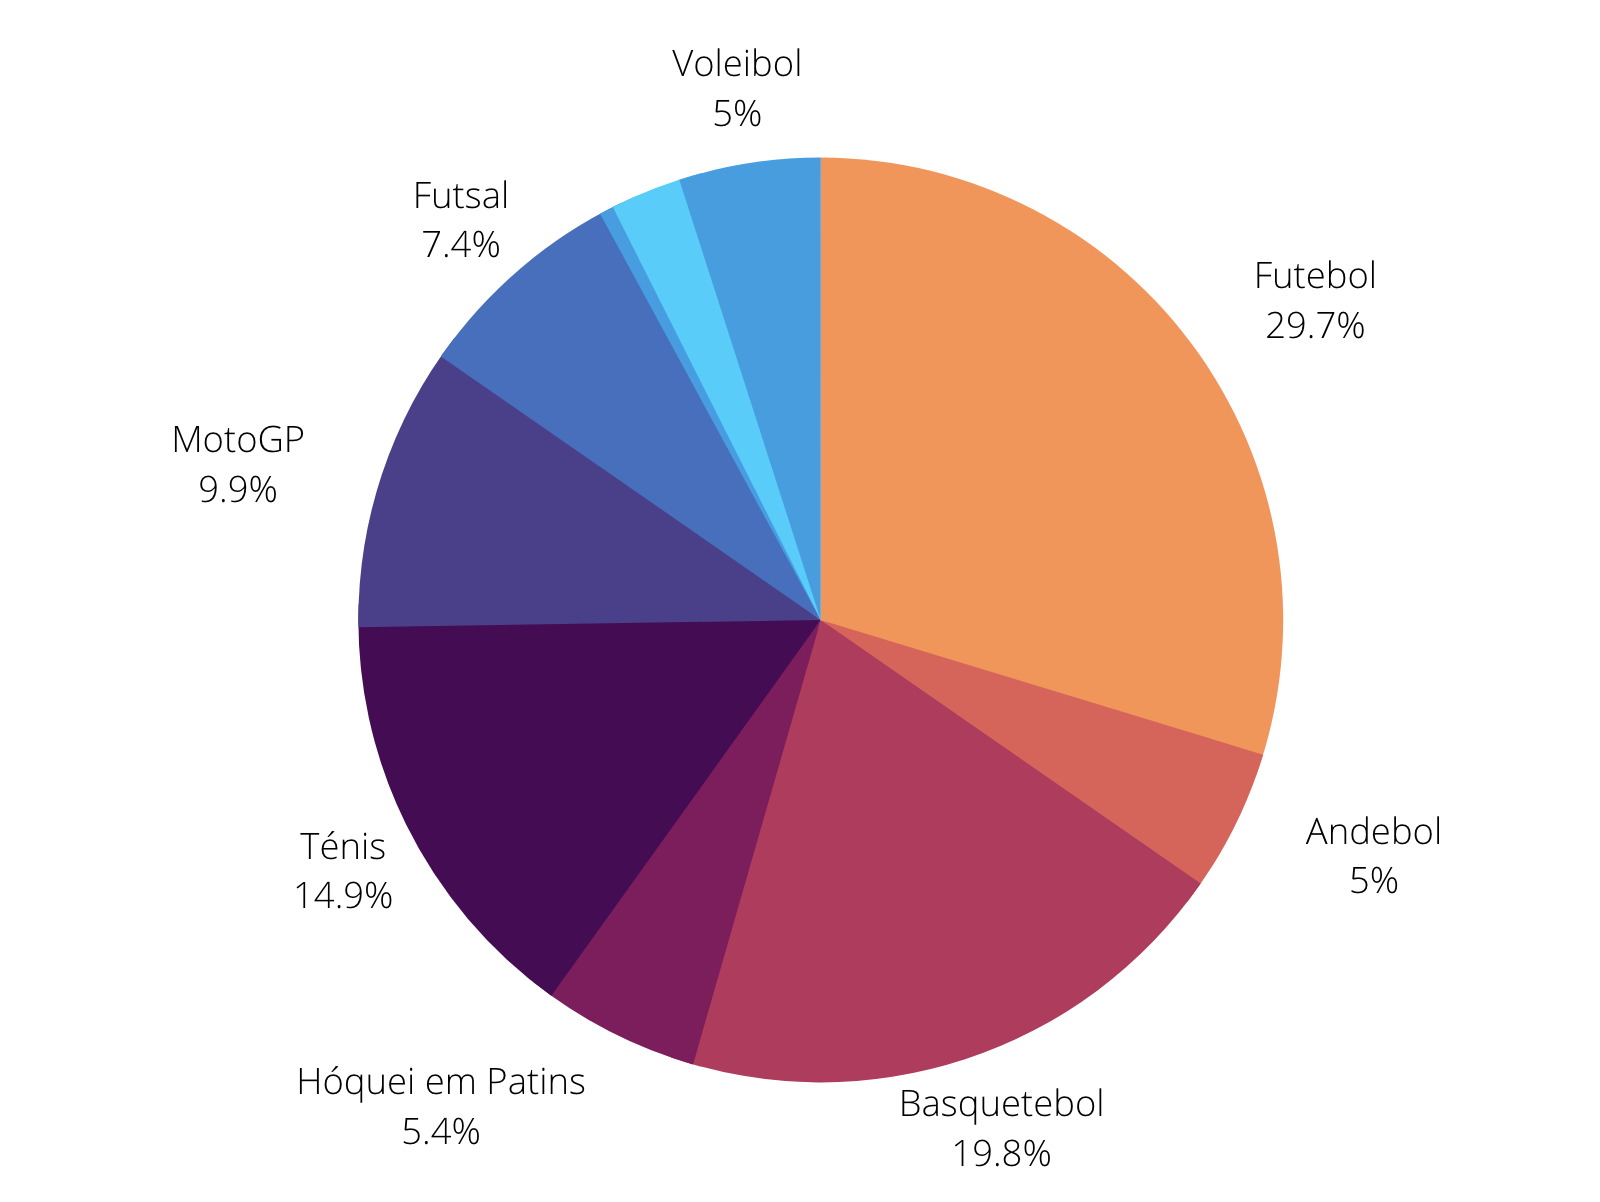
\includegraphics[width=.65\linewidth]{imagens/levantamentoRequisitos/Grafico1.png}
            \caption{Gráfico 1 }
        \end{figure}
    \vspace{20mm}
    \item \textbf{Gostavam de apostar em...}
        \begin{figure}[!htb]
            \centering
            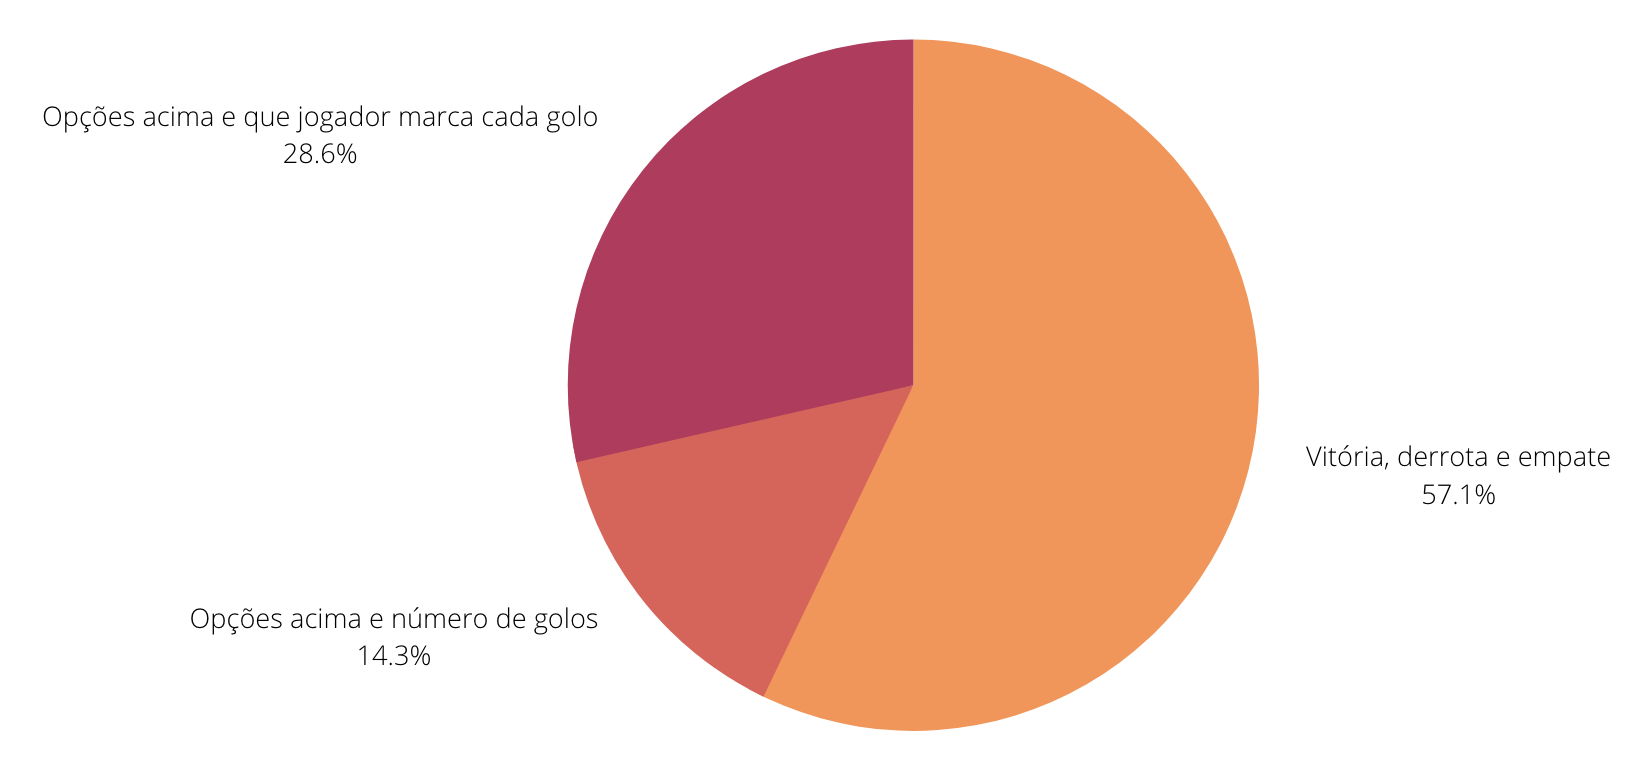
\includegraphics[width=.90\linewidth]{imagens/levantamentoRequisitos/Grafico2.png}
            \caption{Gráfico 2 }
        \end{figure}
        \newpage
    \item \textbf{Gostavam de ter hipótese de fazer mais de uma aposta simultaneamente?}
        \begin{figure}[!htb]
            \centering
            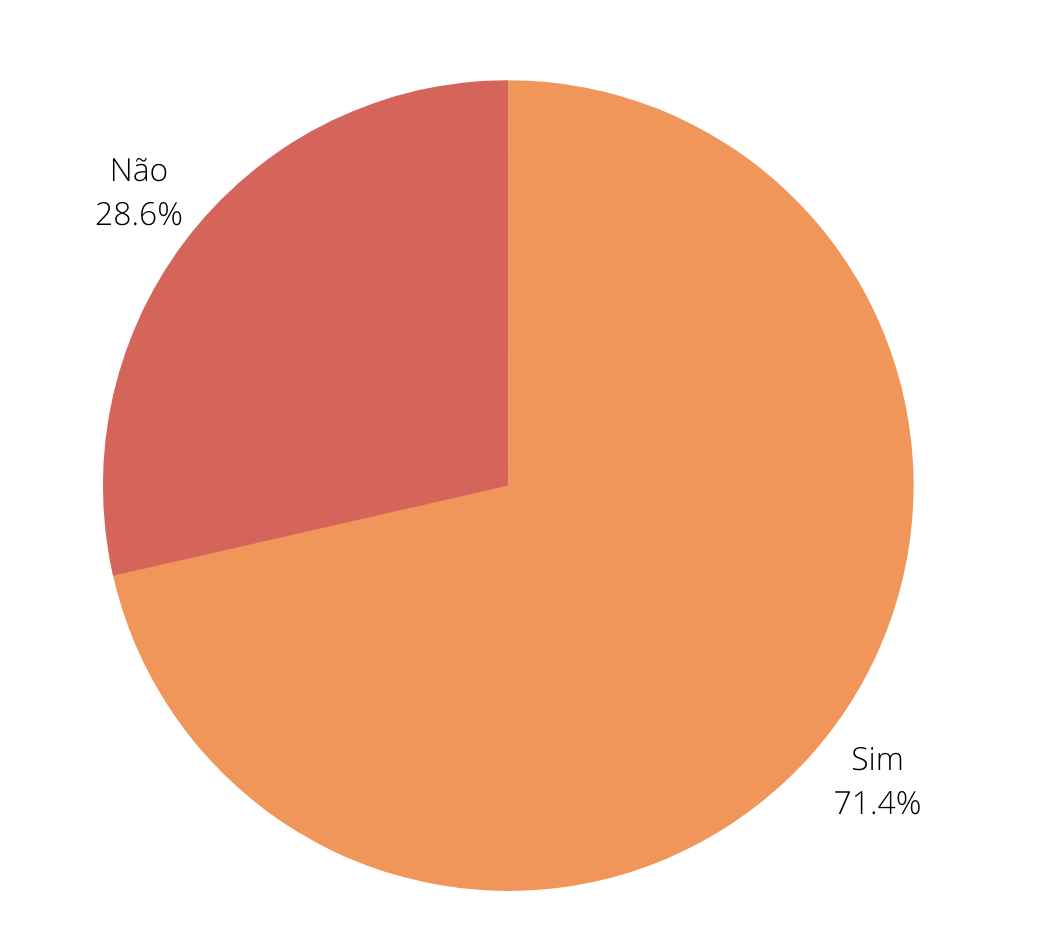
\includegraphics[width=.50\linewidth]{imagens/levantamentoRequisitos/Grafico3.png}
            \caption{Gráfico 3 }
        \end{figure}
\end{enumerate}

\subsection{Entrevista ao diretor da casa de apostas}
A presente entrevista foi elaborada pelos elementos do grupo, de modo a obter informações acerca das necessidades dos nossos clientes, as casas de apostas.
\subsubsection{Transcrição da Entrevista}
Entrevista conduzida ao diretor da casa de apostas \textit{DiBet}.
\begin{itemize}
    \item[] \texttt{ENTREVISTADOR:} Que tipos de desportos é que gostaria de ver no sistema?
    \item[] \texttt{ENTREVISTADO:} Como é de conhecimento geral, o futebol é o desporto mais praticado e adorado do mundo, portanto penso que será indispensável a sua inclusão. Para além deste, considero o basquetebol uma aposta muito interessante e segura a ser considerada. 
    
    \item[] \texttt{ENTREVISTADOR:} Considera a criação de um serviço web ou mobile futuramente uma abordagem interessante?
    \item[] \texttt{ENTREVISTADO:} Sem dúvida, penso que a criação de um serviço web é indispensável. Desta forma, os apostadores podem aceder ao serviço de apostas em qualquer equipamento.
    
    \item[] \texttt{ENTREVISTADOR:} Gostaria que a equipa de programadores estivesse disponível para dar suporte à aplicação criada futuramente?
    \item[] \texttt{ENTREVISTADO:} Sim, conto com uma equipa que esteja disponível para dar assistência ao sistema e para futuramente expandi-lo. 
    
    \item[] \texttt{ENTREVISTADOR:} Considera importante o sistema expandir as apostas a outros desportos consoante a demanda?
    \item[] \texttt{ENTREVISTADO:} Sim, dependendo da afluência dos meus clientes ao sistema pode ser interessante ter um sistema mais abrangente.
\end{itemize}

\subsubsection{Resumo} A entrevista conduzida ao diretor da casa de apostas foi muito esclarecedora, deu-nos uma ideia mais concreta do que é indispensável incluir no sistema a ser desenvolvido assim como o que pode vir a ser escalável.

\section{Personas}

\subsection{Persona Carlos Moreira} 

\textbf{Nome: }Carlos Moreira 

\textbf{Idade: }30 anos

\textbf{Estado Civil: }Solteiro

\textbf{Habilitações Académicas: }Mestrado em Engenharia Biomédica

\textbf{Profissão: }Engenheiro Biomédico

\textbf{Hobbies: }Fazer apostas desportivas online

\textbf{Residência: }Reside sozinho em Esposende\vspace{5mm}

\textbf{Estilo de vida: } O Carlos é um homem dedicado à sua profissão, trabalha arduamente todo dia. Quando chega a casa, sozinho e com poucos amigos, dedica-se a estudar jogos de basquetebol para fazer as melhores apostas. Sempre adorou o desporto porém o trabalho levou a melhor e já não pratica tanto como gostaria. 


\subsection{Persona João Silva} 

\textbf{Nome: } João Silva

\textbf{Idade: }26 anos

\textbf{Estado Civil: }Solteiro

\textbf{Habilitações Académicas: } 12º Ano

\textbf{Profissão: } Assistente de Oficina Automóvel

\textbf{Hobbies: } Ver MotoGP, Futebol, jogar futebol.

\textbf{Residência: }Reside com os pais em Lisboa\vspace{5mm}

\textbf{Estilo de vida: } O João é amante de um estilo de vida boémio, apreciador da vida noturna. Quando não se encontra na oficina, dedica-se a ver videos no youtube sobre desportos motorizados e futebol, tentando sempre antecipar o resultado dos eventos no fim de semana. Sempre teve o sonho de ser piloto de motociclos, ainda que desde cedo, percebeu que muito dificilmente teria as oportunidades necessárias em Portugal, dedicando-se assim ao ofício de reparação e preparação de carros e motas.

\subsection{Persona Joana Melo} 

\textbf{Nome: } Joana Melo

\textbf{Idade: }36 anos

\textbf{Estado Civil: } Casada

\textbf{Habilitações Académicas: } Licenciada em Ciências da Comunicação

\textbf{Profissão: } Gerente de Loja de Fotografia, blogger em part-time.

\textbf{Hobbies: } Fazer yoga, ver futebol, Fotógrafa amadora, blogger.

\textbf{Residência: }Reside com o marido no Algarve\vspace{5mm}

\textbf{Estilo de vida: } Fanática por futebol e fotografia desde jovem, a Joana acompanha regularmente eventos de futebol nacionais e europeus, sendo uma paixão que partilha com o seu marido. 

\section{Introspeção}
Nesta secção foi feito o levantamento de requisitos através de diferentes estratégias definidas pelos elementos da equipa. Este levantamento foi realizado, agregado e por fim, foi selecionada a informação mais relevante para o projeto em questão.
\par
As entrevistas feitas foram revistas e validadas de forma a verificar se reúnem as características necessárias das partes interessadas. Destes passos resulta um conjunto de requisitos importantes a implementar na nossa aplicação.
\end{document}